\documentclass[twoside,nogutter]{glasgowthesis}
%\documentclass[twoside,hidelinks]{glasgowthesis}
% ^^ draft shows overfilled boxes (but disables links)
% ^^ replace "oneside" with "twoside" to set the gutter correctly for
%    two-sided printing.
% ^^ add "nogutter" option for digital copy (without binding offsets),
%    if printed copy is twoside, use [twoside,nogutter] for digital copy.
% ^^ add "hidelinks" option to remove coloured links (e.g. for printing)

%%%
% Packages

\usepackage{graphicx}
\usepackage{amsmath}
\usepackage{amssymb}
\usepackage{color}
\usepackage{bookmark}
\usepackage{hyphenat} % for \hyp{} instead of "-".

%%%
% Bibliography

% import package and set some options
\usepackage[minnames=1,maxnames=5,style=numeric-comp,sorting=none,backend=bibtex]{biblatex}

% set path to database
\bibliography{bibliography.bib}

%%%
% SI units

% import package
\usepackage[separate-uncertainty=true]{siunitx}

% for nice display of negative symbol in equations
\sisetup{
   detect-mode,
   detect-family,
   detect-inline-family=math,
}

%%%
% List of symbols, definitions, etc.

% import package
\usepackage[acronym,nomain]{glossaries}

% make the list
\makeglossaries

%%%
% superscript th, st, nd, rd, etc.
\usepackage[super]{nth}

%%%
% Hyperlinks
%
% (This should be as close to the end of the package imports as possible - see https://www.tug.org/applications/hyperref/manual.html)

% import package
\usepackage{hyperref}
\hypersetup{
  colorlinks=true,
  linkcolor=blue,
  filecolor=magenta,      
  urlcolor=cyan
}

%%%
% Fix silly LaTeX space/punctuation behaviour with custom commands
%
% The command '\xspace' should be added to the end of custom commands which lack arguments, to make LaTeX put a space after the command's output.
\usepackage{xspace}

%%%
% Smaller text in captions
\usepackage[font=small]{caption}

%%%
% Subcaptions
\usepackage{subcaption}

%%%
% Wrapping text around figures
\usepackage{wrapfig}

%%%
% Formatting of ordinal numbers, i.e. 1st, 2nd, 3rd, as superscripts
\usepackage[super]{nth}

%%%
% Chemical symbols
\usepackage[version=3]{mhchem}

%%%
% Code listings
% https://www.ctan.org/tex-archive/macros/latex/contrib/listings/
\usepackage{listings}

%%%
% Custom commands

% command to make plural versions of commands (http://tex.stackexchange.com/questions/259287/how-to-define-a-newcommand-that-expands-into-another-newcommand)
% e.g.
% 	\makename[es]{veggie}{potato}
% makes the commands \veggie (=potato) and \veggies (=potatoes)
\newcommand{\makename}[3][s]{%
  \expandafter\newcommand\csname #2\endcsname{#3\xspace}%
  \expandafter\newcommand\csname #2s\endcsname{#3#1\xspace}%
}

% red, italic, bold - for notes
\newcommand{\note}[1]{\textcolor{red}{\emph{[\textbf{Note: }#1]}}}

% blue, normal text - for statements that need fact-checked
\newcommand{\checkme}[1]{\textcolor{blue}{#1}}

% naive with diaeresis
\newcommand{\naive}{na\"ive\xspace}

% et al.
% (and a backslash to prevent TeX thinking a new sentence starts afterwards)
\newcommand{\etal}{et~al.\@}

% Michelson interferometer
\newcommand{\MI}{Michelson interferometer\xspace}

% Fabry-Perot with accent
\newcommand{\FP}{Fabry-P\'{e}rot\xspace}

% Fabry-Perot Michelson interferometer
\newcommand{\FPMI}{Fabry-P\'{e}rot Michelson interferometer\xspace}

% Dual-recycled Fabry-Perot Michelson interferometer
\newcommand{\DRFPMI}{Dual-recycled Fabry-P\'{e}rot Michelson interferometer\xspace}

% Sagnac Speedmeter
\newcommand{\SSM}{Sagnac speedmeter\xspace}

% Sagnac Speedmeter experiment
\newcommand{\SSMEXPT}{Sagnac speedmeter experiment\xspace}

% AEI 10m prototype
\newcommand{\AEIPROTOTYPE}{AEI \SI{10}{\meter} prototype\xspace}

% Glasgow 10m prototype
\newcommand{\GLASGOWTENM}{Glasgow \SI{10}{\meter} prototype\xspace}

% Matlab
\newcommand{\MATLAB}{Matlab\xspace}

% title, contents, etc.
\frontmatter
%%%
% Document

\begin{document}

%\pagestyle{empty}
%\pagenumbering{gobble}

\title{Enhancing the Sensitivity of Future Interferometric Gravitational Wave Detectors}
\author{Sean Stephan Leavey}
\date{Month Year}

\maketitle

\cleardoublepage

\input{"00-abstract.tex"}
%\addcontentsline{toc}{chapter}{Abstract}

\newpage
\input{"00-acknowledgements.tex"}
%\addcontentsline{toc}{chapter}{Acknowledgments}

\cleardoublepage
\vspace*{1.75in}
\begin{flushright} Dedication. (Is what you need.)\end{flushright}


%\pagenumbering{roman}
%\setcounter{page}{1}

% -----------------------------------------------------------------------------
\newpage

\vspace*{1.75in}
\begin{center} {\bf Creative Commons Licence}\end{center}
\noindent I hereby grant permission under the following terms...

\begin{description}
\item Sean Stephan Leavey\ \\ \ \\ \ \\
\hrule
\end{description}
\newpage

% -----------------------------------------------------------------------------

% import glossary terms
\input{"00-definitions.tex"} 

% -----------------------------------------------------------------------------
\newpage
%\thispagestyle{empty}

\addcontentsline{toc}{chapter}{Preliminaries}

% change contents title to lower case
\renewcommand{\contentsname}{Table of contents}
\tableofcontents

\listoftables
\addcontentsline{toc}{section}{List of tables}

\listoffigures
\addcontentsline{toc}{section}{List of figures}

\printglossaries
\addcontentsline{toc}{section}{List of acronyms and symbols}

% -----------------------------------------------------------------------------
\cleardoublepage

% Number chapter boomarks
\bookmarksetup{numbered}

\section*{\label{c:intro:thesisstatement}Thesis statement}
\addcontentsline{toc}{section}{Thesis statement}

\input{"00-statement.tex"}

% main chapters
\mainmatter
\chapter{\label{c:gw-detection}Gravitational waves}

\section{Event GW150914}
One billion years ago a pair of black holes, one with \num{36} solar masses and the other with \num{29} solar masses, merged into a single black hole with \num{62} solar masses. The missing energy equivalent to \num{3} solar masses was radiated away in the form of gravitational waves.

At 09:50:45 \gls{UTC} on \nth{14} September 2015, gravitational waves from the event passed through the \LIGO{} Livingston detector, perturbing the mirrors by \SI{e-18}{\meter} and creating a signal large enough for the electronics controlling the interferometer to detect the ripple in space time more than \num{23} times above the background noise. Seven milliseconds later, the same wavefront passed the \LIGO{} Hanford detector and moved the mirrors in the opposite direction. At that moment, for the first time in human history, a gravitational wave had been detected.

From the gravitational waveform witnessed at the \LIGO{} sites it was possible to determine the type and parameters of the waves' source. The waveforms for \emph{\GWFIRSTEVENT{}}, as it became known, are consistent with a binary black hole merger where they are swept up in frequency before creating a loud ``chirp'' signal as shown in Figure\,\ref{fig:gw150914}. The signal was only above each detector's background noise for the last few \SI{}{\milli\second} of this process. Not only did \LIGO{} make the first observation of a gravitational wave, it also made the first detection of a binary black hole system and found the missing experimental proof of Einstein's theory of general relativity. The window into the universe opening up due to \LIGO{} and the worldwide network of gravitational wave detectors in operation and under assembly, \GEO{}, \VIRGO{} and \KAGRA{}, represents an opportunity to study the universe in a completely new way. Some secrets have already been discovered, but there are surely more to be uncovered.

\begin{figure}
  \centering
  \includegraphics[width=\columnwidth]{graphics/generated/from-python/10-gw150914.pdf}
  \caption[Measured strain from the LIGO Hanford and Livingston detectors around the time of event \GWFIRSTEVENT{}]{\label{fig:gw150914}Measured strain from the \LIGO{} Hanford and Livingston detectors around the time of event \GWFIRSTEVENT{}, the first recorded gravitational wave in history. Once a promising signal is identified, a cluster of compute nodes work to find the best fitting waveform from precomputed template banks representing the various combinations of the system's parameters. The waveforms calculated from numerical relativity are shown in the lower panel representing the best fit parameters.}
\end{figure}
% data from https://losc.ligo.org/events/GW150914/

\section{General relativity and gravitational waves}
A consequence of Einstein's theory of general relativity, gravitational waves are produced by changes in the quadrupole moment of a distribution of mass. Changes in the lower order monopole and dipole terms are forbidden due to energy and momentum conservation, meaning that the effect a gravitational wave has on spacetime is to stretch it in one direction while contracting it in another. This strain can be expressed as a linear combination of ``plus'' and ``cross'' polarisation terms, shown for an initially circular ring of test particles as a function of phase angle in Figure\,\ref{fig:gravitational-wave-polarisation}.

\begin{figure}
  \centering
  \includegraphics[width=\columnwidth]{graphics/generated/from-svg/10-gravitational-wave-polarisation.pdf}
  \caption[Plus and cross polarisations of a propagating gravitational wave]{\label{fig:gravitational-wave-polarisation}Plus and cross polarisations of a propagating gravitational wave. As the wave travels, it stretches spacetime in one direction while contracting it in the other in an elliptic behaviour. A gravitational wave's propagation can be described as a linear combination of the two polarisations.}
\end{figure}

Gravitational waves from Earth-bound mass distributions, including the Earth itself, are not even remotely detectable. The strain in spacetime produced by such objects is so weak that there is no hope for us to make such a detection with any known technology. A good estimate for the strain produced by a pair of rotating objects is given in \cite{Sathyaprakash2009} as:
\begin{equation}
  \label{eq:happrox}
  h \lesssim \frac{2 G \left( M v^{2} \right)_{\text{nonspherical}}}{c^4 r},
\end{equation}
where $G$ is the gravitational constant, $\left( M v^{2} \right)_{\text{nonspherical}}$ is the kinetic energy associated with the non-spherical parts of the source, $c$ is the speed of light and $r$ is the distance to the source. To get an idea of what the spacetime strain would be for man-made sources, we can consider as in \cite{Sathyaprakash2009} the case of two cars of mass $M = \SI{e3}{\kilo\gram}$ attached to opposite ends of a rod of length $d = \SI{10}{\meter}$, spinning about its centre in a centrifuge at a frequency of $f = \SI{10}{\hertz}$. The tangential velocity of the cars will be around $2 \pi f d \approx \SI{600}{\meter\per\second}$. Placing the detector one wavelength away, and using Equation\,\ref{eq:happrox}, the strain turns out to be around $\SI{4e-43}{}$. To be able to detect such a strain the current most sensitive detectors, \ALIGO{}, would require an improvement in sensitivity of \SI{20}{} orders of magnitude, which is clearly ludicrous.

A pair of solar-mass objects orbiting each other at \SI{100}{\hertz} within \SI{50}{\mega\lightyear} produces a strain of only one part in \SI{e21}{}, which is a strain only now detectable after decades of detector development, and a feat once thought impossible in the early \nth{20} Century. It is only the waves produced by the most massive objects in the universe which we have any chance of detecting: black holes, compact binary neutron stars and supernovae amongst others. Even then, gravitational radiation is only produced by the presence of a changing quadrupole moment, and so only a subset of sources that happen to be in coalescence or contain surface asymmetries produce waves we have the ability to detect.

\section{Multi-messenger astronomy}
From Equation\,\ref{eq:happrox} we can see that gravitational waves propagate with a $\frac{1}{r}$ law, in that the amplitude of a wave decays as the linear inverse of distance $r$. Contrast that to electromagnetic (\gls{EM}) radiation, with which virtually all astronomy has thus far been conducted, where the $\frac{1}{r^2}$ law limits sensitivity. Combined observations in the \gls{EM} and gravitational wave spectrum\textemdash so-called \emph{multi-messenger} astronomy\textemdash allows researchers to learn even more about the universe by using information gathered from one set of detectors to make targeted searches with the other. So-called \emph{\gls{EM} follow-up} can be carried out after a gravitational wave detection to learn more about the source, and visual observations of events such as supernovae can focus the analysis effort of the vast quantities of detector data produced by the gravitational wave observatories. The long term goal of researchers in the field of astronomy is for a worldwide network of gravitational wave detectors to compliment the existing network of \gls{EM} telescopes.

\section{Development of the gravitational wave detector}
Using the \emph{local Lorenz} gauge an incident gravitational wave can be described as a change in length between two test masses. The primary degree of freedom a gravitational wave excites is the differential mode of the space separating the test masses, \LMINUS{}, which can be defined in terms of the position of the test masses $x_{\textrm{A}}$ and $x_{\textrm{B}}$ as:
\begin{equation}
  \label{eq:darm}
  \textrm{\LMINUS{}} = \frac{x_{\textrm{A}} - x_{\textrm{B}}}{2}.
\end{equation}
The strain of an incident gravitational wave can be determined from this change in length.

The first attempts to detect gravitational waves began with Joseph Weber's studies in the 1960s with his \emph{Weber bar} \cite{Weber1960}. This was a device developed to act as a direct strain meter, with incident gravitational waves exciting modes between the two ends of the bar effectively forming the test masses. Piezoelectric sensors placed on the surface of an aluminium cylinder convert changes in length into electrical signals. Whilst the expected change in length of such a cylinder from gravitational radiation would in most cases be tiny, the resonant frequency of the cylinder, typically in the kilohertz range, acts to enhance the amplitude of the length change at nearby frequencies. The sensitivity of such a bar as a function of frequency is determined in part by its quality factor (Q), with a necessary trade-off being made between peak sensitivity (high Q) and detection bandwidth (low Q). As sources of gravitational radiation are almost universally weak, the only reasonable hope of making such a detection is to choose a high Q material and hope for a favourable signal frequency.

The original resonant bar detectors were evolved over time to become cryogenic, to decrease the effect of thermal noise; and spherical, to maximise the test mass's Q. Despite such improvements the peak sensitivity of state-of-the-art resonant bar detectors was surpassed by \emph{interferometric} gravitational wave detectors in 2003 \cite{Pitkin2011} after it was shown that \emph{second generation} detectors improving upon the initial designs would offer superior sensitivity across a much wider bandwidth \cite{Harry2002a}. The interferometer was first suggested as a means for gravitational wave detection shortly after the introduction of the Weber bar\footnote{The first known example being by Gertsenshtein and Pustovoit in the Soviet \emph{Journal of Experimental and Theoretical Physics} in 1962.}, but efforts to build prototypes and understand the significant sources of noise only gained momentum in the 1970s \cite{Moss1971, Weiss1972}.

\subsection{\label{sec:gw-interferometry}The gravitational wave interferometer}

% keep this here - it's referenced throughout this section
\begin{figure}
  \begin{center}
    \begin{subfigure}{.3\textwidth}
      \includegraphics[width=\columnwidth]{graphics/generated/from-svg/10-michelson.pdf}
      \caption{Simple \MI{}}
      \label{fig:mi}
    \end{subfigure}
    \hfill
    \begin{subfigure}{.3\textwidth}
      \includegraphics[width=\columnwidth]{graphics/generated/from-svg/10-fabry-perot-michelson.pdf}
      \caption{\FPMI{}}
      \label{fig:fpmi}
    \end{subfigure}
    \hfill
    \begin{subfigure}{.3\textwidth}
      \includegraphics[width=\columnwidth]{graphics/generated/from-svg/10-dual-recycled-fabry-perot-michelson.pdf}
      \caption{\DRFPMI{}}
      \label{fig:drfpmi}
    \end{subfigure}
    \caption[The evolution of the gravitational wave detector]{The evolution of the gravitational wave detector. Figure\,\ref{fig:mi} shows the simple \MI{} used since the famous Michelson and Morley experiments of the 1880s, and proposed for gravitational wave detection in early literature. Figure\,\ref{fig:fpmi} shows a \MI{} with the addition of \FP{} arm cavities to enhance sensitivity. Figure\,\ref{fig:drfpmi} shows a \FPMI{} with the addition of recycling mirrors.}
  \end{center}
\end{figure}

Figure\,\ref{fig:mi} shows the \MI{} topology that all current detectors are based on. Gravitational waves modulate the phase of the interferometer light in the arms, and the amount of modulation depends on the ratio of the light's frequency $f_0$ and the gravitational wave frequency $f_g$. A \MI{} can be made by taking coherent light from a laser, splitting it into two parts then shining one on a mirror. Comparing the phase of the reflected light field to the other light field it is possible to detect passing gravitational waves by an additional phase accumulation on the returning light on top of the expected round trip phase with respect to the first. The change in the arm length $\Delta L$ with respect to the nominal length $L$, which gives the gravitational wave's \emph{strain}, is then given by:
\begin{equation}
  \label{eq:freq-to-length}
  \frac{\Delta L}{L} = \frac{\Delta f}{f},
\end{equation}
where $\Delta f$ is the measured change in laser frequency at the detector normalised by the carrier frequency $f$. Gravitational wave induced phase modulation can also be described with the \emph{transverse traceless} gauge as a change in the refractive index of the light between the test masses. The effect is equivalent.

The simple \MI{} design has a number of disadvantages. Using the standard ground-based gravitational wave detector wavelength ($\lambda_0 = \SI{1064}{\nano\meter}$), when the arm length is optimal for a gravitational wave of frequency $\SI{e3}{\hertz}$, the wave's phase modulation effect on the light is of the order $\frac{f_0}{f_g} = \frac{\SI{e14}{}}{\SI{e3}{}} = \SI{e11}{}$ which gives an estimate of the strain enhancement in the interferometer. Gravitational radiation from likely sources reaches us with strain of at most \SI{e-21}{} meaning that the interferometer's electronics would need to be capable of making a phase measurement of at least \SI{e-10}{\radian}: a very difficult feat. Furthermore, the optimal antenna length for a gravitational wave detector is $\frac{c_0}{4 f_g}$ \cite{Abbott2016a}, as with electromagnetic antennae, and so for this frequency the arm would ideally be \SI{75}{\kilo\meter}. This is clearly impractical for ground based detectors.
% from http://imprs-gw.aei.mpg.de/miscellaneous/05_downloads/imprs-lecture-weeks/march-2014/experimental-gw-physics/modulation/

\subsubsection{\label{sec:fabry-perot-cavities}\FP{} arm cavities}
One way to simultaneously reduce the phase measurement requirement and the effective arm length is to use \FP{} cavities\footnote{Other techniques were tested around this time such as delay lines, though they were found to have additional technical challenges for no greater benefit \note{cite something from Garching?}.}. \FP{} cavities increase a photon's effective path length by reflecting it many times between two partially transmitting mirrors. While this improves on the \MI{}'s phase measurement requirement by approximately the cavity gain (a function of the mirror reflectivities, typically of the order \num{100} to \num{1000}), this still leaves the interferometer susceptible to fluctuations in the laser's frequency which are indistinguishable from signal. This problem can be addressed through the use of \FP{} cavities in the arms of a \MI{}. By placing two arm cavities at the reflected and transmitted ports of the beam splitter the light that recombines at the output port contains out-of-phase copies of the laser's frequency fluctuations which cancel out. A \emph{\FPMI{}} is shown in Figure\,\ref{fig:fpmi}.

\subsubsection{\label{sec:power-recycling}Power recycling}
The \FPMI{} can provide good cancellation of laser frequency noise and good sensitivity to differential arm length fluctuations, but one problem is still apparent: the vast majority of the light that recombines at the beam splitter is sent back towards the laser, where it samples the position of input optics not necessarily isolated from the ground and interferes with the laser crystal. This light is typically rejected by means of a Faraday isolator, leading to power loss. To save this light from being lost, an additional mirror can be placed at the input to reflect the light returning to the laser back into the interferometer. This technique is called \emph{power recycling}, and it increases the power in the arms by approximately the gain of the cavity the power recycling mirror forms with each arm's input mirrors. The \emph{first generation} \ILIGO{}, \IVIRGO{} and \IVIRGO{} detectors were \PRFPMI{}s.

\subsubsection{\label{sec:signal-recycling}Signal recycling}
Signal recycling is an evolution on the \PRFPMI{}, which involves the placement of a \emph{signal recycling} mirror at the output port of the interferometer, whereby the signal created at the output of the interferometer can be enhanced in a certain frequency band by the creation of an additional \emph{signal recycling cavity} \cite{Meers1988}. The signal recycling mirror's transmissivity and position can be modified to determine the frequency range over which this enhancement occurs due to the dynamics of the cavity \cite{Buonanno2001}.

\subsubsection{Dual recycling with \FP{} arm cavities}
The natural combination of power and signal recycling with the \FPMI{} leads to the \emph{\DRFPMI{}} shown in Figure\,\ref{fig:drfpmi}. This is the topology that provides the greatest sensitivity, either broadband or narrowband depending on the tuning of the signal recycling cavity, for a given laser power, arm length and mirror mass; it is therefore the topology employed in current generation detectors. The use of \emph{dual recycling} was initially demonstrated in both table-top and suspended prototype experiments \cite{Strain1991, Heinzel1998, Freise2000}, and later a full-scale dual-recycled \MI{} detector was demonstrated at \GEO{} \cite{Heinzel2002, Grote2004}. The \ALIGO{} detectors were the first to fully implement the \DRFPMI{} topology.

\section{Overview of current efforts}
As of the time of writing the \ALIGO{} detectors are online and commissioners are working towards reaching the design sensitivity. \AVIRGO{} is due to begin science operations towards the end of 2016, with \KAGRA{} due to follow in 2019. \GEOHF{} has been operational in the years since the initial detectors stopped for upgrades, and is now transitioning into a detector-scale prototype facility. Planning is also under way to build an \ALIGO{} detector in India. The eventual network of detectors is shown in Figure\,\ref{fig:detector-network}.

Beyond this generation, plans are afoot to build facilities which will push the sensitivity of the gravitational wave detector to the limit, with the so-called \emph{third generation} detectors. A European collaboration is working towards the \emph{\ET{}} \cite{ET2011} and the \LSC{} is working towards \emph{\LIGOCE{}} \cite{Dwyer2015}. Efforts are also under way to complement the ground-based detectors with a space-based counterpart with significantly enhanced low frequency sensitivity, \emph{\ELISA{}} \cite{Amaro-Seoane2012}. Together, the network of ground- and space-based detectors will provide unprecedented sensitivity from frequencies of \SI{}{\milli\hertz} to \SI{}{\kilo\hertz}, presenting the ability to study the universe in unparalleled fidelity.

\begin{figure}
  \centering
  \includegraphics[width=\textwidth]{graphics/generated/from-python/10-detector-network.pdf}
  \caption[Worldwide detector network]{\label{fig:detector-network}Worldwide detector network. \GEO{}, \LHO{} and \LLO{} are operational, whilst \VIRGO{} and \KAGRA{} are being commissioned and \INDIGO{} is under construction. The locations of the \ET{} and \LIGOCE{} are as yet undecided.}
\end{figure}

\section{Thesis structure}
This thesis outlines work conducted with the goal of improving the sensitivity of future gravitational wave observatories.

Chapter\,\ref{c:instrumentation} introduces some theoretical foundations and motivation for the work presented in the rest of this thesis. Chapter\,\ref{c:waveguides} presents an investigation into \emph{waveguide} mirrors which offer a large potential improvement in Brownian thermal noise over conventional dielectric mirrors. One downside is the potential presence of a coupling effect between transverse motion and reflection phase. This chapter presents an experiment conducted to measure this coupling in order to give a clearer picture of this type of mirror's potential use in future gravitational wave facilities.

The next set of chapters, \ref{c:speedmeter-intro}, \ref{c:speedmeter-control} and \ref{c:esd-concept}, present experimental research into a new type of gravitational wave interferometer: the \SSM{}. Chapter\,\ref{c:speedmeter-intro} introduces the concept in more detail and presents an overview of an ongoing proof-of-principle experiment taking place in Glasgow. Chapter\,\ref{c:speedmeter-control} highlights an important technical problem with the \SSM{} configuration which is not present with current detectors: that the controller cannot determine the displacement of the cavity mirrors at low frequencies, leading to loss of sensitivity. A solution to the problem is presented through the modelling of the complete control system using existing measurements of the response and noise of the apparatus as well as estimates for noise in the experiment as fully assembled, backed by numerical simulations. Finally, Chapter\,\ref{c:esd-concept} outlines the architecture and construction of experimental apparatus to test a new actuator design to be used in the \SSMEXPT{}: a plate capacitor electrostatic actuator. Designs and tests of high-voltage equipment to create the required test mass actuation are presented \note{along with some preliminary results}.

The main body of the work concludes with Chapter\,\ref{c:et-lf-control} where the current state of the sensing and control design for the low frequency interferometer as part of the planned Einstein Telescope facility is presented. This interferometer is to be primarily sensitive to frequencies below \SI{10}{\hertz} where existing detectors are dominated by seismic noise. Here, the state of the art sensing, controls and actuators found in the current generation of detectors are revisited through the use of numerical simulations.

Finally, the appendices provide additional information for the enthusiastic reader to support the main work. Appendix\,\ref{a:interferometry} provides a mathematical description of a basic interferometer and derives some useful figures of merit used throughout the work to describe interferometers. Appendix\,\ref{a:simulation-tools} discusses the differences between the two main numerical simulation tools used for the presented work in Chapters \ref{c:speedmeter-intro}, \ref{c:speedmeter-control} and \ref{c:et-lf-control}. A conclusion is provided in Chapter\,\ref{c:conclusion}.
\chapter{Sensitivity and noise in gravitational wave interferometers}
\label{c:instrumentation}

To achieve maximum sensitivity in an interferometric gravitational wave detector to a particular type of signal the parameters of the optics, arm lengths and light fields must be considered alongside the characteristics of the signals and noise and the controllability and robustness of the resultant design. This chapter describes some of the considerations to be made in the design of detectors to provide the basis on which the rest of this thesis will build. Section\,\ref{sec:ifo-foundations} details the state in which an interferometer must be brought in order to be sensitive to gravitational waves and the means of keeping it there; Section\,\ref{sec:ifo-noise} introduces the limiting noise sources in ground-based gravitational wave detectors and the physical processes at play; Section\,\ref{sec:ifo-response} discusses ways to improve the sensitivity of interferometers in the frequency bands of interest; and Section\,\ref{sec:sub-sql-techniques} introduces concepts in order to reduce the most challenging noise source arising from the quantum nature of light.

\section{\label{sec:ifo-foundations}Interferometer foundations}
The effect that the output light from an interferometer has on a sensor (e.g. a photodetector) as some variable is modulated is termed its \emph{response}. As discussed in Chapter\,\ref{c:gw-detection} the most important response to consider in gravitational wave interferometry from an astrophysical perspective is that of the differential motion of the arms (\gls{DARM}) to the sensor at the output port. The response has a dependence on the input light power but it varies as a function of frequency due to the presence of additional \emph{cavities} used to enhance or suppress the response in a given frequency band.

\subsection{Measurement of interferometer length fluctuations}
The propagation of an electromagnetic wave can be represented by its complex-valued electric field amplitude $E$ in time and space:
\begin{equation}
  \label{eq:em-propagation}
  E = E_0 \text{e}^{\text{i} \left( \omega t - kx \right)},
\end{equation}
where $\omega$ is the wave's angular frequency, $i$ is the imaginary unit, $t$ is time, $k = \frac{2 \pi}{\lambda}$ is the wave number and $x$ is the coordinate in the direction in which $E$ is measured. An arbitrary phase offset defined with respect to some point is contained within the complex-valued maximum field amplitude, $E_0$.

Typically the underlying amplitude of a particular interferometer signal can only be inferred from the light power measured by a sensor. A simple example is the measurement of mirror displacement in a \MI{} \emph{via} the photocurrent output of the photodetector. The measured power $P$ in this case would be:
\begin{equation}
  P = E^{\ast} E.
\end{equation}
Equation\,\ref{eq:em-propagation} can be simplified to a sinusoidal function with real maximum field amplitude $E'_0$ and phase offset $\phi$:
\begin{equation}
  \label{eq:em-propagation-real}
  E' = E'_0 \cos \left( \omega t - kx + \phi \right),
\end{equation}
and in this way we can express the measured power as the square of the real field amplitude, i.e. $P = E'^2$.

Assuming that laser light with amplitude described by Equation\,\ref{eq:em-propagation-real} is incident upon the beam splitter shown in the \MI{} in Figure\,\ref{fig:mi}, the light returning to the beam splitter having reflected from the north and east arms, $n$ and $e$, respectively, would be:
\begin{align}
  E'_n &= -\frac{E'_0}{\sqrt{2}} \cos \left( \omega t - 2kL_n \right) \\
  E'_e &= \frac{E'_0}{\sqrt{2}} \cos \left( \omega t - 2kL_e \right)
\end{align}
where we employ a particular reflection phase convention such that a negative coefficient is gained on the light reflected from one side of the beam splitter, to conserve energy (see Appendix\,\ref{a:reflection-phase}). We can also express $L_n$ and $L_e$ in terms of the average arm length $L = \frac{L_n + L_e}{2}$ and differential length $\delta L = L_n - L_e$:
\begin{align}
  E'_n &= -\frac{E'_0}{\sqrt{2}} \cos \left( \omega t - 2k \left( L + \frac{\delta L}{2} \right) \right) \\
  E'_e &= \frac{E'_0}{\sqrt{2}} \cos \left( \omega t - 2k \left( L - \frac{\delta L}{2} \right) \right).
\end{align}

The superpositions of the light from the arms leaving the beam splitter towards the input laser, $E'_{\text{input}}$, and the light leaving at the output port, $E'_{\text{output}}$, are then:
\begin{equation}
  \begin{split}
    E'_{\text{input}} &= \frac{E'_{e} - E'_{n}}{\sqrt{2}} \\
                      &= E'_0 \cos \left( \omega t - 2kL \right) \cos \left( 2k \frac{\delta L}{2} \right)
  \end{split}
\end{equation}
\begin{equation}
  \begin{split}
    E'_{\text{output}} &= \frac{E'_{e} + E'_{n}}{\sqrt{2}} \\
                       &= -E'_0 \sin \left( \omega t - 2kL \right) \sin \left( 2k \frac{\delta L}{2} \right).
  \end{split}
\end{equation}
A real photodetector is not quick enough to measure changes in intensity at the frequency of the light. Instead, it sees the time averaged square of the field. The photodetector power at the output as a function of $\delta L$, $P_{\text{output}}$, is:
\begin{equation}
  \label{eq:mich-p-out}
  P_{\text{output}} \left( \delta L \right) = \frac{P_0}{2} \left( 1 - \cos \left( k \delta L \right) \right),
\end{equation}
where $P_0$ is the power of the incident laser light, showing that the signal from the differential arm length is encoded in the power of the light present at the output port. Note that implicit in this derivation is the assumption that the arms are both perfectly reflective. When the optics within the interferometer have different reflectivity, the calculation becomes more complicated and it is then more practical to use a simulation tool, as discussed in Appendix\,\ref{a:simulation-tools}.

\subsection{\label{sec:operating-point}Optimal operating point}
The phase change created by the difference in the lengths of the arms shown in Equation\,\ref{eq:mich-p-out} as $k \delta L$ can be expressed as a combination of a \emph{static} tuning $\alpha$ and the phase change created by incident gravitational waves, $\delta \phi_{\text{GW}}$, i.e.:
\begin{equation}
  k \delta L = \alpha + \delta \phi_{\text{GW}}.
\end{equation}

The static tuning $\alpha$ is the differential arm phase at which the interferometer is nominally held. In experiments where sensitivity can be sacrificed for simplicity, often it is practical to keep the interferometer in the state commonly referred to as ``half way up the fringe''. Here, the interferometer's arms are nominally tuned \SI{45}{\degree} out of phase such that the output signal oscillates about the midpoint between crest and trough of the superposition waveform at the output. As the gradient is steepest at this point (as specified by Equation\,\ref{eq:mich-p-out}), any small changes to the relative arm length of the \MI{} result in a significant difference in power at the photodetector. This operating point, however, is not optimal in terms of \emph{sensitivity} to arm length fluctuations. The static light power at this operating point contributes significant \emph{shot noise} at the output, $P_{\text{shot, out}}$, given by:
\begin{equation}
  P_{\text{shot, out}} = \sqrt{2 h f_0 P_0},
\end{equation}
where $h$ is Planck's constant and $f_0$ is the light frequency. The optimally sensitive operating point is therefore not simply one which maximises the signal gradient, but rather one which maximises the \emph{signal-to-noise ratio} (\gls{SNR}). It turns out that the reduced signal in the case of the operating point close to the \emph{dark fringe}, where light from the two arms interferes destructively, is more than compensated for by the lack of shot noise such that the overall sensitivity is better. Interferometer operation near the dark fringe is the basis of \emph{\gls{DC} readout}, described in the next section, which is the standard measurement technique for all current generation detectors.

\subsection{\label{sec:readout}Readout}
% chapter 4 points here
Note that the light power at the output shown in Equation\,\ref{eq:mich-p-out} in the cosine of the change in arm length is symmetrical and so displacements $\pm \delta L$ yield identical changes in light power. As the interferometer must be held at the dark fringe in order to maximise sensitivity, a controller would require a \emph{bipolar} error signal providing a different response for motion in a different direction. The purpose of the \emph{readout} technique is to facilitate a bipolar error signal.

Another benefit certain types of readout can provide is access to the displacement information in a particular \emph{quadrature} of the output light. Signal (and noise) can in general be encoded in both the amplitude and phase of the light, representing the light's quadratures. When the ratio between optical power and mirror mass is high this information is primarily contained within the phase quadrature, and when significant optomechanical interactions are present either with lighter mirrors or higher laser power the information can be encoded as a linear combination of the phase and amplitude quadratures. Some readout techniques provide access to an arbitrary readout quadrature where the signal can be maximised with respect to the noise, while others have a quadrature fixed by the interferometer parameters.

There are two types of readout technique. \emph{Heterodyne} readout involves the use of a second light frequency used as a \emph{local oscillator} for the primary light frequency that is resonant within the interferometer. This was one of the first techniques used to control laser interferometric gravitational wave detectors \cite{Willke2002}, but due to the presence of \emph{cyclostationary} noise \cite{Niebauer1991} and challenges related to the creation of a stable local oscillator frequency this has since been superseded by \emph{homodyne} techniques as the \gls{DARM} sensor. Homodyne readout involves the use of the carrier frequency as both a signal field and local oscillator, and this leads to some cancellation of noise sources common to the carrier at the expense of additional technical complexity. These techniques are discussed in greater detail in the following subsections.

\subsubsection{Heterodyne readout}
When light with multiple frequency components is incident upon a photodetector the resulting electrical signal shows the \emph{beat signal} between the two components. Assuming that a photodetector has an incident electric field amplitude composed of two frequency components, we get \cite{Freise2010}:
\begin{equation}
  E' = E'_0 \cos \left( \omega_1 t \right) + E'_0 \cos \left( \omega_2 t \right),
\end{equation}
where $\omega_1$ and $\omega_2$ are the two frequencies and $t$ is time. The photodetector measures the power of the field, $P$:
\begin{equation}
  \label{eq:photodetector-beat-power}
  P = {E'}^2 = {E'}_0^2 \left( \cos^2 \left( \omega_1 t \right) + \cos^2 \left( \omega_2 t \right) + \cos \left( \left( \omega_1 + \omega_2 \right) t \right) + \cos \left( \left( \omega_1 - \omega_2 \right) t \right) \right).
\end{equation}
If the difference frequency $\omega_1 - \omega_2$ in Equation\,\ref{eq:photodetector-beat-power} is small, it can be measured by the photodetector. Most heterodyne techniques involve the frequency modulation of a single carrier which creates a series of sidebands offset in frequency from the carrier that beat together at the photodetector. Different resonant conditions for the sidebands with respect to the carrier allow some to act as phase discriminants for others, and with suitable \emph{demodulation} at the photodetector these can be used to sense displacement in the interferometer arms.

\subsubsection{\label{sec:homodyne-readout}Homodyne readout}
One way in which to picture homodyne readout is as a heterodyne readout with $\omega_1 = \omega_2$. It is possible to create a homodyne local oscillator by using a second laser with identical frequency to the first, though it is usually beneficial to use the same laser to benefit from coherent noise cancellation.

The first large scale application of homodyne readout in gravitational wave detectors was \emph{\gls{DC} readout} \cite{Fricke2012}, where a detuning (\emph{\gls{DC} offset}) is intentionally created within the interferometer's arms to allow for some of the carrier light to appear at the output port where it acts as a local oscillator to the rest of the carrier that contains the gravitational wave signal. This technique has the benefit that the local oscillator is filtered by the interferometer which suppresses certain types of noise, but it involves the intentional introduction of a classical light field at the output port. Another homodyne technique, \emph{balanced homodyne detection}, involves the picking off of a fraction of the interferometer's input for use as a local oscillator. In this case, signal encoded in the light leaving the interferometer can be mixed with the local oscillator without the need for a \gls{DC} offset. The \gls{DC} readout technique is used in current generation detectors but for future interferometers it is possible that balanced homodyne detection will become the norm \cite{Gard2016}.

The technical implementation of \gls{DC} readout is discussed in more detail in Chapter\,\ref{c:et-lf-control}, and balanced homodyne readout forms the basis for the experiment introduced in Chapter\,\ref{c:speedmeter-intro}.

\subsection{Control}
In order for the interferometer to be kept at its operating point the readout signal representing the positions of the test masses must be fed back to test masses actuators. These actuators typically take the form of voice coils, piezoelectric materials and other mechanical transducers. The ubiquitous technique for the control of the positions of mirrors is \emph{linear negative feedback}, where the readout signal is passed through a \emph{servo} which applies frequency-dependent filtering to enhance or suppress particular components and invert the signal before it is sent to the actuators. If the control system is designed to react quickly to test mass motion, the interferometer can be held almost exactly at the operating point where the error signal from the readout is nulled. Equation\,\ref{eq:mich-p-out} shows that small arm displacements lead to linear changes in the output power, and this is true for most readout techniques too. Effective control of the interferometer holds it within this linear region to ensure that the readout is maximally sensitive to the displacement of the arms.

Control strategies are discussed in greater detail in Chapters \ref{c:waveguides}, \ref{c:speedmeter-control} and \ref{c:et-lf-control}. Appendix\,\ref{a:control} also introduces some background concepts useful for the understanding of the control strategies presented in these chapters.

\section{\label{sec:ifo-noise}Measurement noise in interferometers}
The ``signal'' in an interferometer is the collection of electrical oscillations representing the particular variable of interest which, in most cases, represents the motion of the test masses in the arms. ``Noise'', on the other hand, refers to the unwanted oscillations that appear in the measurement independent of such a variable. The sensitivity of an interferometer is set by the magnitude of the signal with respect to the noise, the \gls{SNR}, defined in the context of test mass displacement in Section\,\ref{sec:operating-point}.

Gravitational wave interferometers are limited by a plethora of noise sources across the spectrum. The knowledge of the limiting noise sources gained from the science runs undertaken by the initial generation of interferometric detectors (\LIGO{}, \VIRGO{}, \GEO{} and \TAMA{}) has fed in to the design of the current second generation (\ALIGO{}, \AVIRGO{} and \KAGRA{}).

The creation of \emph{noise budgets} from theoretical descriptions and measurements of sources is a useful way to examine how noise influences the sensitivity of an experiment. The noise budget for \ALIGO{}'s design configuration is shown in Figure\,\ref{fig:aligo-noise-budget}. At its most sensitive frequencies, \ALIGO{} is limited by \emph{quantum} and \emph{thermal} noise, whilst at lower frequencies the motion of the ground from seismic sources sets the limit. Careful design involving specially selected materials and techniques has reduced thermal noise arising from the mirror coatings and suspensions and technical noise associated with electronics and facilities. Quantum noise sets the fundamental limit given the available light power and mirror masses utilised in the detectors. In order to improve the sensitivity beyond the limit set by quantum noise, approaches that involve changing the nature of the quantum interactions within the interferometer have to be implemented. Important noise sources useful for the rest of this thesis are discussed throughout this section.

\begin{figure}
  \centering
  \includegraphics[width=\columnwidth]{graphics/generated/from-python/20-aligo-noise-budget.pdf}
  \caption[Advanced LIGO noise budget]{\label{fig:aligo-noise-budget}\ALIGO{} noise budget presented by \gls{GWINC} \cite{gwinc}. Greater sensitivity to gravitational waves is achieved by having lower residual strain noise. The incoherent sum of the noise sources leads to the overall sensitivity of the interferometer, and this is shown in \checkme{black}. All of the noise sources shown have some frequency dependence, and optimal sensitivity in a detector is reached by designing the experiment in such a way as to minimise the noise sources in the frequency band of interest. The creation of budgets like this from theoretical descriptions of noise sources is a useful way in which to understand how they affect the sensitivity.}
\end{figure}

\subsection{\label{sec:noise-via-loss}Noise arising from loss and uncertainty}
The development of quantum theory showed that the universe contains a continuous spectrum of quantum fluctuations at all frequencies. Virtual photons are constantly being created and annihilated in all space, albeit with an average energy of zero, producing the measurement uncertainty predicted by quantum mechanics. Collections of mirrors within interferometers create local filters of this quantum spectrum which allow a subset of vacuum modes to circulate. Virtual photons are able to enter the interferometer via its \emph{loss points}, where light can escape the interferometer, just as virtual photons created within the interferometer are allowed to leave. As the vacuum fluctuations are uncorrelated with the motion of the test masses, non-unity reflectivity of optics, scattering and other photon loss effects within an interferometer lead to the intrusion of vacuum noise.

In lasers, a pumped electromagnetic field creates a state which can be used as the input light for an interferometer. This typically involves pumping the field into the \emph{coherent} state in which the average laser amplitude and phase quadratures are well defined, and noise arises from the presence of virtual photons with arbitrary amplitude and phase in the pumped field leading to an uncertainty in the number of photons output from the laser.

In materials, phonons \checkme{arising from thermal energy uncertainty} have a similar effect to vacuum fluctuations and lead to thermal noise.

In general, the noise arising from fluctuations is quantified by the fluctuation dissipation theorem developed in the early \nth{20} Century, which shows that the noise spectral density due to fluctuations,
\begin{equation}
  S_{\text{fluc}} \propto \frac{T}{Q},
\end{equation}
is related not only to the temperature $T$, but also to the quality factor $Q$ relating to the loss of the material.

The effect of noise on the interferometer can be calculated by quantifying the magnitude of noise entering at the loss point and propagating this noise to the signal detection point where it can potentially mask the signal. The noise at a photodetector is therefore the sum of noise propagated from each point of loss to the readout point. The way in which some forms of noise can enter a \MI{} and propagate to the output port is shown in Figure\,\ref{fig:modelling-noise}.

\begin{figure}
  \centering
  \includegraphics[width=\columnwidth]{graphics/generated/from-svg/20-modelling-noise.pdf}
  \caption[Some entry points for noise in a \MI{}]{\label{fig:modelling-noise}Some entry points for noise in a \MI{}.}
\end{figure}

\subsection{Thermal noise}
Thermal noise arises from loss in materials used to reflect and focus light and to suspend test masses, where photons given a phase change due to thermal excitations are allowed to enter the interferometer and propagate to the sensors.

Thermal noise arises from a material's \emph{loss angle}, which is the imaginary part of the Young's modulus relating applied stress to the corresponding strain of the material. Material with a high loss angle results in an applied stress creating an associated strain at a different time, and during this time the incident light can accumulate noise via thermal fluctuations of the material. The most significant thermal noise contributions in gravitational wave detectors arises from the test mass optical coatings and suspensions.

\subsubsection{\label{sec:coating-thermal-noise}Coating thermal noise}
In the conceptual design for the first generation of gravitational wave detectors such as GEO-600 \cite{Willke2002} the designers were not aware that thermal noise associated with the reflective coatings on mirrors would play a significant role in the sensitivity of the interferometers. For a long time it was known that thermal noise would contribute to the sensitivity of the detectors, particularly from the bulk material forming the test masses, but it soon became clear as the detectors were being commissioned that thermal noise arising from the reflective mirror coatings would dominate the thermal noise associated with the test masses in the frequency band of interest despite forming only a tiny fraction of the test masses by volume. Investigations conducted by Harry \etal{} \cite{Harry2002, Harry2007}, among others, concluded that mechanical loss present in the numerous dielectric coating stacks on the test masses required for high reflectivity led to Brownian noise creating a limit to the sensitivity of detectors across a wide range of frequencies. Contributions from thermoelastic noise, arising from the thermal expansion coefficient of the materials of the coatings \cite{Braginsky1999a}, and thermorefractive noise, arising from the change in refractive index caused by fluctuations in the material's temperature \cite{Braginsky2000a}, produce further noise contributions which will become more important as coatings with improved Brownian noise contributions are developed.

Over the past two decades, efforts have been made to both quantify and reduce coating thermal noise. Particular interest is being paid to the study of coatings for cryogenically cooled mirrors, such as the sapphire (\ce{Al_2O_3}) test masses to be used in the Japanese detector \gls{KAGRA} \cite{Somiya2012}. A loss peak in the mirror material silica (\ce{SiO_2}), for detectors until recently ubiquitous, occurs at low temperature. This makes the material unsuitable for cryogenic use, as mechanical loss will couple into the light within the interferometer and make its way to the detection port. Other materials such as sapphire do not feature this loss peak and provide lower thermal noise than silica at room temperature for a given mirror design. Coating noise is also proportional to temperature, so cryogenically cooled mirrors can offer better performance. Additionally, crystalline coatings made from compounds such as \ce{AlGaAs} can offer future detectors a coating thermal noise reduction of up to 3 over current state of the art \cite{Cole2013} if technical challenges in their manufacturing can be overcome.

The dominant contribution to coating noise in gravitational wave detectors comes from Brownian noise, given as \cite{Harry2002}:
\begin{equation}
  \label{eq:coating-brownian-psd}
  S_{\text{x, coating}} = \frac{2 k_B T}{\pi^{3/2} f} \frac{1}{w Y} \left( \phi_{\text{sub}} + \frac{1}{\sqrt{\pi}} \frac{d}{w} \left( \frac{Y'}{Y} \phi_{\text{para}} + \frac{Y}{Y'} \phi_{\text{perp}} \right) \right),
\end{equation}
for Boltzmann constant $k_B$, temperature $T$, frequency $f$, beam size $w$, Young's modulus $Y$, loss angle $\phi$ and coating thickness $d$. The Young's moduli are split into components representing the coatings and substrate, $Y$ and $Y'$, and the loss angles are split into parallel and perpendicular components in the coatings, $\phi_{\text{para}}$ and $\phi_{\text{perp}}$, and substrate, $\phi_{\text{sub}}$, respectively. The measurement and interaction between these components is an active area of research. Figure\,\ref{fig:aligo-noise-budget} shows coating Brownian noise jointly dominating the noise at frequencies around \SI{70}{\hertz}.

A mirror topology which avoids the use of many alternating coating layers can potentially offer an improvement in noise performance. Mirrors employing grating structures can resonantly reflect light with less coating material than similarly performing dielectric mirrors \cite{Mashev1985}, though at the expense of additional technical complexity in their utility in gravitational wave detectors \cite{Leavey2015}. Chapter\,\ref{c:waveguides} discusses a form of grating mirror for use in interferometers.

\subsubsection{\label{sec:sus-thermal-noise}Suspension thermal noise}
The test masses in audio-band gravitational wave detectors are suspended from pendulum systems, and current generation observatories (with the notable exception of \KAGRA{}) all utilise fused silica fibres, a technique pioneered for \GEO{} \cite{Barr2002}. The reason for the use of this material is that the thermal noise present within the previously used steel loops was high enough to impart significant displacement noise to the test mass in the gravitational wave channel, with the noise becoming dominant at frequencies around \SI{100}{\hertz} where the interferometer would otherwise be most sensitive \cite{Hammond2012}. Due to its high quality factor, fused silica has reduced mechanical loss and therefore lower noise. Figure\,\ref{fig:aligo-noise-budget} shows that suspension thermal noise is no longer a dominant noise source, unlike in \ILIGO{}.

As \KAGRA{} will be a cryogenic detector, it does not gain the same noise benefit from using fused silica. Instead, it will use crystalline sapphire which offers similar noise performance at low temperatures.

At higher frequencies, suspension \emph{violin modes} have a significant influence on the measured noise \cite{Robertson2002}. A violin mode with high quality factor can resonantly enhance noise such that it dominates all other sources in a narrow band at frequencies starting around a few hundred \SI{}{\hertz}\footnote{Figure\,\ref{fig:aligo-noise-budget} appears to show that violin modes are not dominant, however the narrow linewidth of the noise is such that the resolution is insufficient to show the effect.}. This is reduced through the use of heavier test masses, which push the violin mode frequencies higher, away from the detection band, and with special monitoring techniques \cite{Sorazu2010}.

\subsection{\label{sec:quantum-noise}Quantum noise and the Standard Quantum Limit}
Arising from the Heisenberg Uncertainty Principle, the quantum noise present within a classical interferometer\footnote{Note the misnomer: a \emph{classical} interferometer can still be limited by \emph{quantum} noise. The name refers to the readout technique, namely the measurement of classical light power to determine displacement.} limits its sensitivity. One of the results of quantum theory is that two non-commuting observables cannot be simultaneously known to full precision. For two operators $\hat{O}_+$ and $\hat{O}_-$, there exists an error $\epsilon$:
\begin{equation}
 \left[ \hat{O}_+, \hat{O}_- \right] = \epsilon;
\end{equation}
this means that the observables contain correlated components and as such cannot be considered entirely separate entities. Measuring one observable automatically influences the other, leading to the well-known \emph{Heisenberg Uncertainty Principle}:
\begin{equation}
 \left| \Delta \hat{O}_+ \right| \cdot \left| \Delta \hat{O}_- \right| \geq
\frac{1}{2} \left| \epsilon \right|,
\end{equation}
where $\Delta$ represents the uncertainty in the given operator, in this case defined as the standard deviation.

\subsubsection{\label{sec:operator-uncertainty}Position, momentum, phase and photon number uncertainty}

In the field of gravitational wave interferometry there are two pairs of operators of particular importance, namely the position and momentum operators, $x$ and $p_x$, and the photon number and phase operators, $n$ and $\phi$, respectively. The canonical commutation relation between $x$ and $p_x$ is given as:
\begin{equation}
 | \Delta x\left( t \right) | \cdot |\Delta p_x\left( t \right) | \geq
\frac{\hbar}{2},
 \label{eq:heisenburguncertainty}
\end{equation}
where $\hbar$ is the reduced Planck constant. Consider a position measurement of a free mirror of mass $m$ being perturbed by a signal of frequency $f$. If a measurement is made at time $t$ and then again at time $t + \Delta t$, the uncertainty on the latter can be expressed in terms of the uncertainty in momentum of the mirror multiplied by the time difference:
\begin{equation}
 \Delta x \left( t + \Delta t \right) = \Delta x \left( t \right) + \Delta p_x
\left( t \right) \frac{\Delta t}{m}.
 \label{eq:heisenburgtime}
\end{equation}
This result shows that the momentum of the mirror at time $t$ influences the position of the mirror at a later time. Since momentum is position scaled by velocity, this leads to a minimum value on which $x \left( t \right)$ can take:
\begin{equation}
 \Delta x \left( t \right) \geq \sqrt{\frac{\hbar \Delta t}{2m}}.
\end{equation}
The key result to highlight here is that, even with an otherwise unperturbed mirror, the momentum imparted by the measurement at time $t$ influences the later measurement at $t + \Delta t$ in such a way that it adds uncertainty. Or, put another way, Equation\,\ref{eq:heisenburguncertainty} expresses that the smaller the error on the position of an observable in a quantum mechanical system, the greater the error on the momentum; and vice-versa. This will become important for new interferometer topologies considered later in Chapter,\ref{c:speedmeter-intro}.

We typically make position measurements indirectly via the change in phase of photons from a laser. In this case, the most appropriate uncertainty relation to use is the photon number-phase relation:
\begin{equation}
  \label{eq:photon-phase-hup}
  \Delta n \Delta \phi \geq \frac{1}{2}.
\end{equation}
Assuming that a photodetector has incident upon it $n$ photons in a given interval, the standard deviation of the number of photons detected per unit time will follow Poisson statistics, i.e. $\Delta n = \sqrt{\bar{n}}$, where $\bar{n}$ is the average photon number calculated by considering many intervals. A single photon has energy $E_P$ given by the standard relation:
\begin{equation}
  E_P = hf,
\end{equation}
and so the power in the beam at a given interval is then:
\begin{equation}
  \begin{split}
    P &= E_P n \\
      &= hfn.
  \end{split}
\end{equation}
The measurement of power is simply the energy multiplied by its complex conjugate, i.e. $P = E^{\ast}E$, and so we can recover the original energy of the light from the measurement of power:
\begin{equation}
  \left| E \right| = \sqrt{hfn}.
\end{equation}
Given that:
\begin{equation}
  \frac{\Delta \left| E \right|}{\Delta n} = \frac{d \left| E \right|}{dn},
\end{equation}
we can obtain the standard deviation of the measured amplitude:
\begin{equation}
  \label{eq:std-dev-amp}
  \begin{split}
    \Delta \left| E \right| &= \frac{d \left| E \right|}{dn} \Delta n \\
                            &= \frac{1}{2} \sqrt{\frac{hf}{n}} \Delta n \\
                            &= \frac{1}{2} \sqrt{hf} \\
                            &= \frac{1}{2} \sqrt{E_P}.
  \end{split}
\end{equation}
Note that this variation does not depend on photon number, and is instead defined only in terms of a fundamental constant and the laser frequency. This is the origin of quantum noise, and the lack of dependence on light power justifies the inclusion of arm cavities in gravitational wave detectors as discussed in Section\,\ref{sec:fabry-perot-cavities}.

The effect the amplitude variation has on the phase uncertainty can be calculated by expressing it as the fractional energy uncertainty:
\begin{equation}
  \label{eq:phase-uncertainty}
  \begin{split}
    \Delta \phi &= \frac{\Delta \left| E \right|}{\left| \bar{E} \right|} \\
                &= \frac{\sqrt{hf}}{2} \frac{1}{\sqrt{hf \bar{n}}} \\
                &= \frac{1}{2 \sqrt{\bar{n}}} \\
                &= \frac{1}{2 \Delta n}.
  \end{split}
\end{equation}
From the last line in Equation\,\ref{eq:phase-uncertainty} we can recover a result resembling that given in Equation\,\ref{eq:photon-phase-hup}:
\begin{equation}
  \label{eq:photon-phase-hup-min}
  \Delta n \Delta \phi = \frac{1}{2}.
\end{equation}
The reason for the $=$ in Equation\,\ref{eq:photon-phase-hup-min} is that an assumption has been made in Equation\,\ref{eq:std-dev-amp} that the energy uncertainty is made from equal parts amplitude and phase uncertainty. This is called a \emph{coherent state} and this approximates what a standard laser will output\footnote{Actually, lasers are typically quite incoherent on their own, and experimentalists must first ``mode clean'' the light to remove unwanted incoherent states. Mode-cleaning cavities are implemented in some experiments to perform this task.}, albeit alongside significant classical amplitude and phase fluctuations at lower frequencies. Equation\,\ref{eq:photon-phase-hup} contains a $\geq$ and is therefore a general equation representing all states, including \emph{squeezed} states, which will be discussed in Section\,\ref{sec:squeezing}.

\subsubsection{\label{sec:quantum-shot-noise}Quantum shot noise}
As described in Section\,\ref{sec:noise-via-loss}, open ports in the interferometer allow vacuum noise to enter. When this noise is measured by a photodetector it is termed \emph{quantum shot noise}, and it arises directly from the phase uncertainty derived in Section\,\ref{sec:operator-uncertainty}. We change representation from discrete pulses to a continuous measurement made by a laser by representing $n$ in Equation\,\ref{eq:photon-phase-hup-min} as a light power $P$ via the relation
\begin{equation}
  P = \frac{n \hbar \omega_0}{\Delta t}.
\end{equation}
The displacement-equivalent shot noise power spectral density then arises from the phase uncertainty:
\begin{equation}
  \label{eq:shot-noise-psd}
  S_{\text{shot}} = \frac{\hbar c^2}{P \omega_0}.
\end{equation}
As quantum noise arises from vacuum noise\textemdash spontaneous creation and annihilation of photons in the vacuum\textemdash it is a statistical random process and so the shot noise spectral density in Equation\,\ref{eq:shot-noise-psd} has equal power at all frequencies; it is \emph{white} noise.

The detrimental effect of counting statistics due to phase uncertainty is mitigated by an increase in the classical light power within the interferometer. As the noise entering the interferometer is a function of loss and is to first order not dependent upon laser power, higher input power leads to an increase in signal with respect to noise and so the sensitivity is increased.

\subsubsection{\label{sec:quantum-rp-noise}Quantum radiation pressure noise}
Despite being massless, photons impart momentum to mirrors upon reflection proportional to their wavelength. The strongest effect this has on an interferometer is via \emph{\gls{DC} radiation pressure}, which arises from the classical light power circulating within the interferometer. In a suspended interferometer this radiation pressure effect extends the microscopic arm cavity length, with the equilibrium point being defined by the equivalence of the radiation pressure force to the suspension's restoring force.

\emph{Quantum} radiation pressure, on the other hand, arises from the momentum imparted onto mirrors within the interferometer by virtual photons present within the interferometer from the laser and loss points, as shown in Section\,\ref{sec:noise-via-loss}. As with quantum shot noise this effect is related to the input power of the interferometer, but in this case the input power facilitates phase fluctuations that become transformed into displacement noise via the dynamics of the mirror. Mirror dynamics govern the displacement noise due to back-action. The spectrum of noise from virtual photons is white so the energy imparted to the mirror is the same at all frequencies and therefore the effect of radiation pressure follows an inverse frequency relation.

The radiation pressure noise power spectral density is given as \cite{Danilishin2012}:
\begin{equation}
  \label{eq:rp-noise-psd}
  S_{\text{rp}} = \frac{P \hbar \omega_0}{c^2 m^2 \omega^4},
\end{equation}
with reduced mirror mass $m$ and angular frequency of oscillation $\omega = 2 \pi f$. The displacement spectral density, which is $\sqrt{S_{\text{rp}}}$, shows the noise is proportional to $\frac{1}{f^2}$ as expected from a free mass.

\subsubsection{\label{sec:sql}The Standard Quantum Limit}
Note that Equation\,\ref{eq:rp-noise-psd} is proportional to power whilst Equation\,\ref{eq:shot-noise-psd} is inversely proportional to power. This creates a lower bound on the sensitivity of a classical interferometer though a manifestation of the Heisenberg Uncertainty Principle, termed the \emph{standard quantum limit} (\gls{SQL}).

The \gls{SQL} is the point at which the quadrature sum of shot and radiation pressure noise is minimised, and this occurs when the individual components are equal. For each laser power there exists a single frequency at which the \gls{SQL} can be reached. The \gls{SQL} forms a sensitivity limit with amplitude spectral density proportional to $\frac{1}{f}$ which can only be surpassed with special, \emph{sub}-\gls{SQL} techniques. The presence of cavities in the arms of a \MI{} (formed by placing an additional, partially reflecting mirror in each arm) can enhance the power available to be able to reach the \gls{SQL}. In terms of strain, the \gls{SQL} is defined for a \MI{} with arm cavities as \cite{Braginsky1996}:
\begin{equation}
  \label{eq:strainsql}
  h_{SQL} = \sqrt{\frac{8 \hbar}{m \omega^2 L^2}},
\end{equation}
where $L$ represents the \MI{}'s arm length.

The power spectral density for a \MI{} with arm cavities is defined as:
\begin{equation}
  \label{eq:classicalifospectrum}
  S_h = \frac{h^{2}_{SQL}}{2} \left( \frac{1}{\kappa} + \kappa \right),
\end{equation}
where the \gls{SQL} is reached only at a single frequency. The term $\kappa$ is defined as the \emph{opto-mechanical coupling constant}:
\begin{equation}
 \kappa = \frac{I_0}{I_{SQL}} \frac{2 \gamma^4}{\omega^2 \left( \gamma^2 +
\omega^2 \right)},
 \label{eq:optomechanicalcoupling}
\end{equation}
with $I_0$ the laser power at the test masses, $I_{SQL}$ the laser power required to reach the \gls{SQL} and $\gamma$ the arm cavity half-bandwidth. $I_{SQL}$ can be itself defined as:
\begin{equation}
 I_{SQL} = \frac{m L^2 \gamma^4}{4 \omega_0},
\end{equation}
with $m$ the mirror mass, $L$ the arm length and $\omega_0$ the light's angular frequency. The effect of $\kappa$ is described in more detail in Section\,\ref{sec:position-meter-measurement}.

The \gls{SQL} is a locus defined at all frequencies, while the spectral density of a quantum noise limited interferometer touches the \gls{SQL} at only one frequency, defined by the mirror mass, light power, arm length and cavity bandwidth. By injecting more photons into the interferometer to carry more information regarding the motion of the mirrors, we see a smaller shot noise spectral density (we reduce $\Delta n$) whilst we see a larger radiation pressure noise spectral density (we increase $\Delta \phi$) \cite{Caves1981}. This situation is illustrated in Figure\,\ref{fig:sql-vs-input-power} for different input powers.

\begin{figure}
  \centering
  \includegraphics[width=\columnwidth]{graphics/generated/from-python/20-sql-vs-power.pdf}
  \caption[Standard quantum limit and the quantum noise with various input powers]{\label{fig:sql-vs-input-power}The \gls{SQL} for a Michelson interferometer with arm cavities of length \SI{1}{\kilo\meter}, mirrors with reduced mass \SI{50}{\kilo\gram} and optimal frequency \SI{100}{\hertz}, along with quantum noise limited sensitivity curves for three different intracavity powers. The higher the intracavity power, the higher the strain sensitivity can be pushed, but at the expense of higher radiation pressure noise and thus higher optimal frequency for a given interferometer configuration. Quantum non-demolition techniques can be used to surpass the \gls{SQL} (see Section\,\ref{sec:sub-sql-techniques}).}
\end{figure}

An important distinction to make here is that the \gls{SQL} is defined for \emph{uncorrelated} shot and radiation pressure noise. Techniques exist in theory and practice to reduce overall noise by producing correlations between the two effects with so-called \emph{quantum non-demolition} interferometry, and this is discussed in greater detail in Section\,\ref{sec:sub-sql-techniques} and Chapter\,\ref{c:speedmeter-intro}.

\subsection{Other fundamental noise}

\subsubsection{\label{sec:seismic-noise}Seismic noise}
The Earth's surface vibrates with a large amplitude and low frequency \cite{ET2011}. At around \SI{10}{\micro\hertz} tidal forces due to the gravitational interaction between the Earth and Moon dominate the spectrum producing displacements of up to \SI{100}{\micro\meter} \cite{Adhikari2004}. At around \SI{0.15}{\hertz} the swell of the ocean can be measured almost anywhere on the Earth, even far from coasts. These effects produce a large amount of displacement noise at low frequencies which must be filtered.

As seismic noise is large in amplitude, it is able to move test masses in interferometers far enough that they no longer fulfil the resonant condition and lose light power. In almost all audio-band interferometric experiments a large degree of isolation must be utilised to mitigate seismic noise. In Advanced \gls{LIGO}, active platforms sitting atop passive damping materials are used to reduce this noise. Test masses are also suspended from many pendulum stages to isolate higher frequencies such that by \SI{10}{\hertz} the ground motion is suppressed by \checkme{10 orders of magnitude}.

As gravitational waves primarily excite the degree of freedom along the optical axis of each test mass in a \MI{}, homogeneous, vertical surfaces do not couple vertical seismic noise into the gravitational wave channel. Real suspended optics, however, contain imperfections in their manufacturing and couple a small amount of vertical motion into the horizontal direction. In addition, the curvature of the Earth over distances like the \SI{4}{\kilo\meter} arms in \ALIGO{} mean that the local gravitational fields at the \glspl{ETM} are not entirely aligned to those of the \glspl{ITM}, and so to achieve cavity resonance the operating point requires a slight off-horizontal tilt which creates seismic noise coupling. In \ALIGO{} the requirement for vertical to horizontal coupling is to be below \num{1e-3}.

\subsubsection{\label{sec:gravity-gradient-noise}Gravity-gradient noise}
Changes in the density of the ground near the test masses created by seismic noise can couple to the gravitational wave channel via \emph{gravity-gradient} noise, also referred to as \emph{Newtonian} noise. No experiment has successfully been able to decouple this subtle effect from other sources of noise, but it is believed from extensive modelling effort that this noise source will represent a problem particularly for low frequency detectors such as \ETLF{} \cite{ET2011, Hild2011}. Simulations have shown promise in subtraction of gravity-gradient noise inferred from a series of auxiliary witness sensors \cite{Harms2015} as well as a benefit to shaping the profile of the ground near test masses \cite{Harms2014}.

Gravity gradient noise will be discussed in the context of \ETLF{} in Chapter\,\ref{c:et-lf-control}.

\subsection{Technical noise}

\subsubsection{\label{sec:laser-noise}Laser frequency and intensity noise}
A perfect laser would provide output at a single, well defined frequency. In reality such lasers do not exist and their outputs contain spectral impurities. As the laser wavelength is the ``metre stick'' by which we make displacement measurements in interferometers, it is very important to ensure that the laser's wavelength, and therefore frequency, is well defined. Frequency stabilisation control loops involving optics and electronics are usually necessary in high precision interferometric experiments.

Laser frequency noise affects the phase of the output light by creating a beat between waves with different frequencies, created via thermal effects in the laser material. This can be expressed as a time-varying shift $\phi \left( t \right)$ in the underlying wave's phase. This phase transforms into frequency noise via the relation

\begin{equation}
  \Delta f = \frac{1}{2 \pi} \frac{d \phi}{dt}.
\end{equation}

The spectral density of frequency noise can be calculated from the autocorrelation between a frequency fluctuation at time $t$ and another at time $t + \Delta t$, but a simpler method is to realise that the laser is used to measure the cavity length by relating its change in frequency to the change in length via Equation\,\ref{eq:freq-to-length}. Multiplying the relative frequency noise by the difference in arm lengths $\delta L$ gives a first order estimate of the displacement noise created by fluctuations in the laser. Mathematically:
\begin{equation}
  \label{eq:laser-freq-noise}
  x_{\text{freq. noise}} = \delta L \frac{\Delta f}{f}.
\end{equation}

The laser's intensity fluctuates due to similar mechanisms. Thermally driven misalignments within the laser can lead to scattering and the production of higher order modes, which reduce the intensity of the fundamental mode. This has a similar effect on the output as frequency noise, coupling relative intensity noise $\frac{\Delta P}{P}$ directly to the output via the microscopic offset from the dark fringe condition $\delta l$:
\begin{equation}
  \label{eq:laser-int-noise}
  x_{\text{int. noise}} = \delta l \frac{\Delta P}{P}.
\end{equation}

Equations \ref{eq:laser-freq-noise} and \ref{eq:laser-int-noise} show that the level to which the dark fringe condition is satisfied determines the laser noise witnessed at the output. This is because of the cancellation at the beam splitter from noise in the two arms. Laser noise propagates to the beam splitter, where it is split between the arms. Matching the arms macroscopically cancels frequency noise and matching the arms microscopically cancels intensity noise.

\subsubsection{\label{sec:johnson-nyquist-noise}Electronic noise}
Johnson-Nyquist noise arises from loss within electronic conductors. The noise scales with resistance and is characterised in units of \SI{}{\volt\per\sqrthz} by the equation:
\begin{equation}
  v_{\text{n}} = \sqrt{4 k_B T R},
\end{equation}
where $v_{\text{n}}$ is the noise voltage and $R$ is the electrical resistance. The Johnson-Nyquist noise from a resistor in the \SI{}{\kilo\ohm} to \SI{}{\mega\ohm} range is comparable to the noise of some low-noise operational amplifiers at room temperature, and so care must be taken in the choice of passive and active components in the design of electronics to avoid introducing excess fluctuations.

Other electronic noise can arise in integrated circuits used as part of readout electronics in detectors. Current and voltage noise present at the input and output of devices such as operational amplifiers (op-amps) can become larger than the signals being amplified without careful selection of the device for the intended application. This is examined in more detail in Sections \ref{sec:op-amp-noise} and \ref{sec:hv-amplifier}.

\section{\label{sec:ifo-response}Sensitivity of the \MI{}}
The phase accumulated by the light in each of the arms of a \MI{} created by incident gravitational waves as shown in Equation\,\ref{eq:gw-phase-change} is proportional to the power in the arms, and so greater input power leads to greater response at the output (given the caveats regarding quantum noise as discussed in Section\,\ref{sec:quantum-noise}).

As shown in Section\,\ref{sec:gw-interferometry}, the arm length of a \MI{} to provide optimal modulation upon the light field from a passing gravitational wave can be many hundreds of \SI{}{\kilo\meter} for audio band signals. Furthermore, given the standard wavelength $\lambda_0 = \SI{1064}{\nano\meter}$ for which low noise lasers exist, and a gravitational wave strain $h_0 = \num{e-21}$ similar to that of \GWFIRSTEVENT{}, the modulation index will be of the order $\frac{\omega_0}{\omega_g} \approx \num{e12}$ and so the phase of the light will have to be measured at the output port to a precision of around $h_0 \frac{\omega_0}{\omega_g} \approx \SI{e-9}{\radian}$, a difficult feat.

When the interferometer is held at the dark fringe the light from each arm containing common phase changes exits the beam splitter back towards the input. Typically a Faraday isolator is present at the input to dump this light in order to prevent it from accumulating signal from the motion of the input optics and re-entering the interferometer, and so this light would otherwise be lost.

Improvements to the \MI{} design have been made over the past decades in order to address these issues, and these are discussed in the following subsections.

\subsection{\label{sec:fabry-perot-cavities}\FP{} arm cavities}
One way to simultaneously reduce the phase measurement requirement and the \emph{effective} arm length is to use \FP{} cavities. \FP{} cavities increase a photon's effective path length by reflecting it many times between two partially transmitting mirrors. By placing \FP{} cavities in the arms of a \MI{}, as shown in Figure\,\ref{fig:fpmi}, the response can be enhanced in a particular frequency band defined by the cavity parameters. The effect of the cavity on the sensitivity can be characterised by the \emph{finesse} as discussed in Appendix\,\ref{sec:cavity-fom}. Increased cavity finesse leads to a greater number of stored photons over a given period, allowing for greater response to incident gravitational waves, but over a narrower bandwidth than the simple \MI{}. The reflectivity of the mirrors in \FP{} cavities must be chosen to allow for sufficient sensitivity in the desired band; the objective is not simply to maximise the light storage time.

\begin{figure}
  \centering
  \includegraphics[width=0.5\columnwidth]{graphics/generated/from-svg/20-fabry-perot-michelson.pdf}
  \caption[\FPMI{}]{\label{fig:fpmi}\FPMI{} topology.}
\end{figure}

The arm cavities within a \FPMI{} must be held at the operating point just as with a \MI{} to maintain maximum sensitivity. Angular misalignments allow higher order modes of the light field to resonate which can complicate the longitudinal control of the interferometer and can introduce additional noise coupling from mirror surface defects.

\subsection{\label{sec:power-recycling}Power recycling}
As shown in Section\,\ref{sec:operating-point} gravitational wave interferometers are typically held at the dark fringe where the carrier light is rejected by the beam splitter back towards the input laser. It is typical to place a Faraday isolator in the input path to prevent the interferometer from sampling the positions of the input optics used to steer the laser light towards the beam splitter, and so this light is dumped. Once lost this light is not available to sample the positions of the test masses.

To compensate for interferometer light lost towards the input port it is possible to increase the input laser power, but in general appropriate input lasers are already used at the maximum output power that satisfies an experiment's laser noise requirement, and this doesn't solve the underlying loss mechanism: some light will still be dumped by the Faraday isolator. Another approach is to place a \emph{power recycling mirror} at the input to the interferometer which reflects the returning light back into the interferometer by forming a cavity between the recycling mirror and the arms, effectively increasing the power stored there. Used in combination with \FP{} arm cavities this technique can achieve enhanced sensitivity over the standard \MI{}. The power recycling mirror can be calibrated to enhance the carrier power in a band wider than the intended detector bandwidth, and the \FP{} mirrors can be calibrated to set the detector bandwidth. The \emph{first generation} \ILIGO{} and \IVIRGO{} detectors were \PRFPMI{}s.

\subsection{\label{sec:signal-recycling}Signal recycling}
Signal recycling is a similar concept to power recycling, whereby an additional mirror is placed within the interferometer to selectively enhance light in a particular frequency band \cite{Meers1988}. In this case the \emph{signal recycling mirror} is placed at the output port of the beam splitter to create an additional cavity between the output and the arms. This mirror enhances the signal power at the expense of the bandwidth of the arms, as opposed to the carrier enhanced by the use of a power recycling mirror. The signal recycling mirror's transmissivity can be set to determine the frequency range over which this enhancement occurs, and the position of the signal recycling mirror can be tuned to focus this enhancement in either a narrow or broad frequency band \cite{Buonanno2001}.

\subsection{Dual recycling with \FP{} arm cavities}
The natural combination of power and signal recycling with the \FPMI{} leads to the \emph{\DRFPMI{}} shown in Figure\,\ref{fig:drfpmi}. This is the topology that provides the greatest sensitivity in a given band of interest, either broadband or narrowband depending on the tuning of the signal recycling cavity, for a given laser power, arm length and mirror mass; it is therefore the topology employed in current generation detectors. The use of \emph{dual recycling} was initially demonstrated in both table-top and suspended prototype experiments \cite{Strain1991, Heinzel1998, Freise2000}, and later a full-scale dual-recycled \MI{} detector was demonstrated at \GEO{} \cite{Heinzel2002, Grote2004}. The \ALIGO{} interferometers were the first fully implement the \DRFPMI{} topology in detectors capable of sensing gravitational waves.

\begin{figure}
  \centering
  \includegraphics[width=0.5\columnwidth]{graphics/generated/from-svg/20-dual-recycled-fabry-perot-michelson.pdf}
  \caption[\DRFPMI{}]{\label{fig:drfpmi}Dual-recycled \FPMI{}.}
\end{figure}

\section{\label{sec:sub-sql-techniques}Surpassing the Standard Quantum Limit}
Predictions for the population of sources within the range of the advanced detectors show that it is most beneficial to improve the sensitivity at low frequencies \note{need source: perhaps CE or ET-LF designs?}. The strain sensitivity of a \MI{} at low frequencies can be increased through the use of heavier masses as shown by Equation\,\ref{eq:strainsql}, with the strain sensitivity scaling proportionally to $\sqrt{m}$. The use of mirrors larger and heavier than the \SI{40}{\kilo\gram} mirrors used in \ALIGO{} is a considerable technical challenge. The availability of test mass material of suitable quality in such dimensions is not clear, as is the ability for the suspension systems to isolate noise from such large masses.

To improve sensitivity at higher frequencies, Equation\,\ref{eq:shot-noise-psd} shows that laser power can be increased. As with heavier mirrors, this presents technical challenges in laser stability \cite{Hildebrandt2007}, the control of \emph{parametric instabilities} \cite{Evans2015} and the thermal effects associated with absorption in materials \cite{Steinlechner2016}.

To bypass the problems associated with the use of heavier mirrors and more powerful lasers, a number of techniques have been proposed in the literature to increase the sensitivity of interferometers beyond the \gls{SQL} through the use of \emph{quantum non-demolition} (\gls{QND}) techniques \cite{Braginsky1995}. These include the modification of the optics of the interferometer \cite{Kimble2001}, such as through the injection of squeezed light \cite{Caves1981}, variational readout \cite{Vyatchanin1995, Vyatchanin1996} or \SM{}s \cite{Braginsky1990}; and the creation of new light-mirror interactions to increase the response of the interferometer to differential motion of the test masses \cite{Chen2011}.

\subsection{\label{sec:squeezing}Squeezing}
The use of squeezing is an attempt to replace the normally uncorrelated vacuum noise entering the interferometer at the output port with \emph{correlated} noise. By choosing a suitable readout \emph{quadrature}, it is possible to remove some of the quantum noise impinging upon the signal, instead moving the noise terms into the orthogonal, unobserved readout quadrature. Squeezing is particularly favourable in combination with \gls{DC} readout, a combination currently implemented in \GEOHF{} \cite{Willke2006, Affeldt2014}.

To achieve broadband reduction of quantum noise with squeezing it is necessary to inject the squeezed light via filter cavities to provide a frequency-dependent phase shift to the vacuum field \cite{Kimble2001}. These cavities are typically high finesse, which makes the squeezed light particularly susceptible to filter cavity loss \cite{Kwee2014}.

Squeezing has been demonstrated in \GEOHF{} with high duty cycle \cite{Grote2013} and is a planned upgrade for \ALIGO{} in the near future \cite{Miller2015}. The proposed designs for the \ET{} and \LIGOCE{} suggest \SI{10}{\deci\bel} squeezing.

\subsection{Variational readout}
Instead of modifying the input noise at the output port of the interferometer with frequency-dependent squeezing, variational readout achieves broadband sub-\gls{SQL} sensitivity through the use of a homodyne detector with frequency-dependent homodyne angle. The frequency dependence can be achieved in a similar way to squeezing: the output light can be passed through filter cavities in a similar way to squeezed input.

Variational readout can in theory be combined with squeezing either with a fixed squeezing angle \cite{Buonanno2004} or through a complicated frequency dependence of both squeezing and homodyne phase filter cavities \cite{Harms2003}. The use of homodyne readout in gravitational wave detectors, however, is not considered mature enough for upgrades to existing or future facilities, primarily due to the stability requirements for the local oscillator field \cite{Steinlechner2015}.

\subsection{Light-mirror interactions}
\emph{Optical springs} \cite{Braginsky1999, Buonanno2002, Corbitt2007, Rehbein2008, Gordon2015}, \emph{optical inertia} \cite{Khalili2011, Voronchev2012} and \emph{intracavity schemes} \cite{Braginsky1997, Khalili2002, Danilishin2006} have been proposed for use in gravitational wave detectors to improve sensitivity beyond the \gls{SQL} through the creation of interactions between the mechanical rigidity of suspended mirrors and the optical rigidity created by radiation pressure.

The creation of optical springs requires complicated control arrangements. The use of two optical springs to remove the instabilities created by a single spring can relax some of the control requirements but full studies of the effect of noise and the sensitivity on this type of interferometer are not at a stage to be able to predict their use in future detectors.

\subsection{Modification of the interferometer design}
First proposed in 1990 \cite{Braginsky1990}, the measurement of the speed of test masses instead of displacement can lead to a reduction in quantum noise. Proposals for experiments to measure speed were made later and involved the use of an additional optical cavity at the output port of a \MI{} \cite{Braginsky2000, Purdue2002}, termed a \emph{sloshing} cavity, creating an interaction between the main interferometer and the sloshing cavity that samples the test mass coordinates in a way that resembles speed.

In 2003, Chen showed that the Sagnac interferometer contained the necessary characteristics of a \SM{} \cite{Chen2003} and estimated the sensitivity that such an interferometer might achieve when the corner mirrors are replaced with arm cavities to resemble a \FPMI{}. This work was later expanded to include the effect of losses \cite{Danilishin2004, Danilishin2015}.

The \SSM{} is being considered as a potential upgrade for the \ET{} beyond its initial configuration \cite{Wang2013, Huttner2016}, albeit following a polarising topology with linear arm cavities \cite{Danilishin2004} due to the effect of back-scattering in triangular arm cavities \note{do we have a reference for this back-scattering effect?}.

\section{The future of gravitational wave interferometry}
Plans are in place for upgrades to \ALIGO{} after the science run in 2016, when squeezed light injection will be implemented. In the medium term, the interferometer may be adapted to run with cryogenic optics to provide sensitivity at lower frequencies. The \ALIGO{} and \AVIRGO{} detectors already push their current facilities to their limits, however, and so in the long term the goal is to build new facilities with significantly improved sensitivity. A conceptual design study for the \ET{} was completed in 2011 \cite{ET2011}, a new European facility in a triangular, \SI{10}{\kilo\meter} arm configuration, and similar studies for a new \SI{40}{\kilo\meter} \LIGO{} facility are ongoing \cite{Dwyer2015, aligocosmic2016}. These facilities are planned for the late-2020s to early-2030s, and the ongoing research and development work will help to determine the technologies that become part of these detectors. The reduction of quantum and thermal noise and the control of such interferometers will be crucial areas of investigation, and some potential solutions are presented in the rest of this work.
\chapter{Measuring transverse-to-longitudinal phase coupling in waveguide mirrors}
\label{c:waveguides}

\emph{The following chapter has been adapted from \emph{Upper limit to the transverse to longitudinal motion coupling of a waveguide mirror \cite{Leavey2015}}, published in Classical and Quantum Gravity in 2015. The material from the article has been expanded as appropriate for this thesis, but the results presented are identical.}

As shown in the introduction \note{need link}, waveguide mirrors have been shown to offer a reduction in thermal noise over a dielectric mirror offering equivalent reflectivity, at cryogenic temperatures.

\note{Show plot of aLIGO mirror thermal noise from, and discuss, the Heinert paper.}

\begin{figure}
  \centering
  \includegraphics[width=\columnwidth]{graphics/generated/from-python/30-coating-vs-grating-noise.pdf}
  \caption{Coating vs grating noise}
  \label{fig:coating-vs-grating-noise}
\end{figure}

\begin{figure}
  \centering
  \includegraphics[width=\columnwidth]{graphics/generated/from-python/30-individual-factors.pdf}
  \caption{Individual factors}
  \label{fig:individual-factors}
\end{figure}

\section{Transverse to Longitudinal Phase Coupling}
\note{Pillage the paper for a description of this effect.}

\section{Experiment}
\note{Describe experiment}
\subsection{The Pound-Drever-Hall Technique}
As discussed in \note{instrumentation chapter}, heterodyne locking...

\subsection{Suspended Michelson interferometers}
\note{Say why they didn't work.}

\subsection{Off-Axis Voice Coil}
\note{Put results from test of off-axis voice coil force measurements.}

To examine the effect of misalignment of the voice coil and magnet to their shared radial axis, the apparatus shown in Figure \ref{fig:misaligned-voice-coil-experiment} was set up. A rod was placed above the magnet, with the voice coil attached to its end. The magnet was glued to a thick perspex disc attached to the base edge of an upturned plastic cup, to allow the force applied to the magnet to rigidly couple to the base of the cup. The cup was itself placed upon scales accurate to \SI{1}{\micro\gram} and a translation stage with \SI{25}{\micro\meter} accuracy. With the front edge of the voice coil separated by \SI{7.9}{\milli\meter} to the base of the magnet, a series of force measurements were taken. A constant current source of \SI{50}{\milli\ampere} was applied through the coil while incrementing the translation stage in steps of \SI{0.1}{\milli\meter}. The results in Figure \ref{fig:misaligned-voice-coil-results} show that the effect is negligible within the main experiment's misalignment error.

\note{Add coil sweet spot plot}

\begin{figure}
  \centering
  \includegraphics[width=\columnwidth]{graphics/generated/from-svg/30-magnet-offset-experiment.pdf}
  \caption{\label{fig:misaligned-voice-coil-experiment}Experiment to measure the effect of misaligned voice coil actuation.}
\end{figure}

\begin{figure}
  \centering
  \includegraphics[width=\columnwidth]{graphics/generated/from-python/30-magnet-offset.pdf}
  \caption{Change in force as a function of transverse displacement from voice coil axis. A quadratic fit has been applied to the data and the axes shown are with respect to the position and magnitude of the maximum fitted force, following the assumption that this position is nearest to the optimal alignment. This fit is probably a worst case scenario, as the magnet was positioned close to the voice coil's position of maximum force, where the field gradient is quite flat. \checkme{Assuming the voice coils and magnets were aligned within \SI{0.5}{\milli\meter}, the maximum drop in force would have been negligible\textemdash less than 1\%\textemdash and so this explanation can be ruled out.}}
  \label{fig:misaligned-voice-coil-results}
\end{figure}

\note{Use figure of magnet offset results to calculate the maximum force drop that could have been witnessed}

\section{Analysis and Results}
\note{Bayesian stuff...}

\section{Outlook}

The work presented in this chapter shows that waveguide mirrors potentially offer a competitive alternative to dielectric mirrors in future gravitational wave detectors.

\note{Put plot of equivalent angular noise in aLIGO, showing that better suspensions are needed if it were to be used?}

\chapter{\label{c:speedmeter-intro}The \SSMEXPT{}: introduction and technical design}
\chaptermark{\SSM{} introduction}

This chapter introduces the ongoing \SSMEXPT{} in Glasgow and serves as background for the work presented in \cref{c:speedmeter-control,c:esd-concept}. The first half of this chapter discusses the measurement of test mass displacement and speed in the context of interferometers, and compares the sensitivity of the two measurements. The second half details the particular setup employed in the Glasgow experiment.

\section{\label{sec:pos-speed-meters}Position and \SM{}s}

\subsection{\label{sec:position-meter-measurement}Sensitivity of a position meter}
In an ordinary \FPMI{} the motion of each cavity in the longitudinal direction either increases or decreases the round-trip phase of the light in that arm. The phase difference of the two recombined beams at the beam splitter then leads to a signal at the output port proportional to the differential phase which can be measured using a heterodyne or homodyne readout as discussed in \cref{sec:readout}.

The presence of classical light power in the arms leads to \gls{DC} radiation pressure which imparts a force upon the test masses. The reaction of the mirrors' restoring force, either from its pendulum in a suspended experiment or its mount on a table-top experiment, means that the interferometer can be held at the operating point as discussed in \cref{sec:operating-point} by making microscopic corrections to the position of the optic. The output signal can be calculated by considering \emph{input-output relations} which define the effect that input light has at the output given the interferometer dynamics.

\subsubsection{Input-output relations}
We use the \emph{two-photon formalism}~\cite{Caves1985, Schumaker1985} in order to calculate the effect that the interferometer has on the light's amplitude and phase. This represents the input and output in terms of its \emph{cosine} and \emph{sine} quadratures, namely:
\begin{align}
  \vec{a} &=
  \begin{pmatrix}
    a_c \\
    a_s
  \end{pmatrix} \\
  \vec{b} &=
  \begin{pmatrix}
    b_c \\
    b_s
  \end{pmatrix},
\end{align}
where $\vec{a}$ and $\vec{b}$ are the input and output field vectors, respectively, both amplitude spectral density functions with units of \SI{}{\per\sqrthz}. The output for an interferometer can be expressed as the sum of the strain scaled by the interferometer dynamics and the noise present at the detector~\cite{Danilishin2015}:
\begin{equation}
  \label{eq:ifo-output-signal}
  \vec{b} = \frac{\tilde{h}}{\tilde{h}_{\text{SQL}}} \vec{R} + \mathbb{T} \vec{a},
\end{equation}
where $\tilde{h}$ is the power spectral density of the strain applied to the test masses in units of \SI{}{\per\hertz}, normalised to the amplitude spectral density of the \gls{SQL}, $\tilde{h}_{\text{SQL}}$, as presented in \cref{eq:strainsql}; $\vec{R}$ is the (dimensionless) response of the interferometer from strain to the output and $\mathbb{T}$ represents the (dimensionless) transfer matrix of the input fields to the output fields.

The differential arm response, $\vec{R}_{\left( - \right)}$, is given by
\begin{equation}
  \label{eq:fp-mich-response}
  \vec{R}_{\left( - \right)} = \text{e}^{\text{i} \beta_{\text{FP}}} \sqrt{2 \kappa} \vec{H},
\end{equation}
where $\beta_{\text{FP}}$ is the round-trip phase of the light in the arms, $\kappa$ is the optomechanical coupling factor (as introduced in \cref{sec:sql}) and $\vec{H}$ represents the cosine and sine quadratures of the readout angle, $\zeta$:
\begin{equation}
  \vec{H} =
  \begin{pmatrix}
    \cos \zeta \\
    \sin \zeta
  \end{pmatrix}.
\end{equation}

The round-trip phase is defined as
\begin{equation}
  \beta_{\text{FP}} = \arctan{\frac{f}{\gamma_{\text{arm}}}},
\end{equation}
where $f$ is frequency and $\gamma_{\text{arm}}$ is the \FP{} cavity half-bandwidth (see \cref{sec:cavity-fom}).

The effect that the mirror dynamics have on the readout is governed by $\kappa_{\text{MI}}$ defined for a \MI{} in \cref{eq:optomechanicalcoupling}. This models the effect that a force applied to a mirror has on its position. Mirrors suspended from pendulum systems can be approximated at high frequencies to be free masses, where the effect an applied force has on the position is diminished at higher frequencies, and in the case of a \FPMI{} this force-to-displacement filtering effect scales as $\frac{1}{f^2}$ below the cavity's pole frequency, and $\frac{1}{f^4}$ above it.

The term $\mathbb{T}$ can be further broken down:
\begin{equation}
  \mathbb{T} = \text{e}^{2 \text{i} \beta_{\text{FP}}}
  \begin{pmatrix}
    1 & 0 \\
    -\kappa & 1
  \end{pmatrix},
\end{equation}
showing that the optomechanical coupling factor transforms the input $\vec{a}$ in the cosine (amplitude) quadrature into the sine (phase) quadrature governed by the mirror dynamics on its way to the output. The matrix of noise power spectral densities for the quadratures of the light at the output port, $\mathbb{S}$, is given by averaging over all frequencies:
\begin{equation}
  \mathbb{S} = \left< \vec{b} \cdot \vec{b}^{\dag} \right>.
\end{equation}
Expanding the terms we get
\begin{equation}
  \mathbb{S} =
  \begin{pmatrix}
    1 & 0 \\
    -\kappa & 1
  \end{pmatrix}
  \left< \vec{a} \cdot \vec{a}^{\dag} \right>
  \begin{pmatrix}
    1 & -\kappa \\
    0 & 1
  \end{pmatrix},
\end{equation}
where $h$ in \cref{eq:ifo-output-signal} has been set to \num{0} to remove signal.

\subsubsection{Sensitivity of a \FPMI{}}
In the case of \gls{DC} readout as discussed in \cref{sec:homodyne-readout} and used in current generation detectors, the readout angle $\zeta = \SI{90}{\degree}$ represents the phase quadrature:
\begin{equation}
  \vec{H}_{\text{dc}} =
  \begin{pmatrix}
    0 \\
    1
  \end{pmatrix}.
\end{equation}

We can calculate the signal in the absence of noise at the \gls{DC} readout of the \FPMI{}, $O^{\text{dc}}_{\left( - \right)}$, as a function of differential arm cavity strain $\tilde{h}_{\left( - \right)}$ by rearranging \cref{eq:ifo-output-signal}:
\begin{equation}
  O^{\text{dc}}_{\left( - \right)} = \frac{\tilde{h}_{\left( - \right)}}{\tilde{h}_{\text{SQL}}} \text{e}^{\text{i} \beta_{\text{FP}}} \sqrt{2 \kappa_{\text{MI}}}.
\end{equation}
This is shown in \cref{fig:fp-mich-response} for $\tilde{h} = 1$, arm length \SI{1}{\kilo\meter}, mirror mass \SI{40}{\kilo\gram}, laser wavelength \SI{1064}{\nano\meter} and cavity half-bandwidth \SI{250}{\hertz}.

\begin{figure}[htp]
  \centering
  \input{graphics/generated/from-python/40-fp-mich-response.pgf}
  \caption[Response of a \FPMI{} to differential arm cavity motion]{\label{fig:fp-mich-response}Response of a \FPMI{} to differential arm cavity motion. This shows the signal that would appear at a photodetector placed at the output of the interferometer given unit differential motion of the cavity. The cavity provides a signal with the same response for motion at frequencies below the cavity's pole frequency. Beyond the pole, the response is reduced as the motion becomes faster than the cavity's storage time.}
\end{figure}

Normal, unsqueezed vacuum noise at the input has equal noise contributions in the cosine and sine quadratures, and so we can set it to the identity matrix:
\begin{equation}
  \label{eq:unsqueezed-vacuum-amplitude}
  \left< \vec{a}_{\text{vacuum}} \cdot \vec{a}_{\text{vacuum}}^{\dag} \right> =
  \begin{pmatrix}
   1 & 0 \\
   0 & 1
  \end{pmatrix}.
\end{equation}
The matrix of noise power spectral densities of the light quadratures at the output due to quantum noise, $\mathbb{S}_{\text{FPMI}}$, is then
\begin{equation}
  \begin{split}
    \mathbb{S}_{\text{FPMI}} &=
    \begin{pmatrix}
      1 & 0 \\
      -\kappa_{\text{MI}} & 1
    \end{pmatrix}
    \begin{pmatrix}
      1 & 0 \\
      0 & 1
    \end{pmatrix}
    \begin{pmatrix}
      1 & -\kappa_{\text{MI}} \\
      0 & 1
    \end{pmatrix} \\
    &=
    \begin{pmatrix}
      1 & -\kappa_{\text{MI}} \\
      -\kappa_{\text{MI}} & 1 + \kappa^2_{\text{MI}}
    \end{pmatrix}.
  \end{split}
\end{equation}
The noise seen by the \gls{DC} readout is determined by the homodyne angle:
\begin{equation}
  \begin{split}
    S_{\text{FPMI}}^{\text{dc}} &= \vec{H}_{\text{dc}}^{T} \mathbb{S}_{\text{FPMI}} \vec{H}_{\text{dc}}.
  \end{split}
\end{equation}

For \gls{DC} readout, the output noise spectral density is shown in \cref{fig:fp-mich-noise}. This is the combination of radiation pressure noise from the mirrors and shot noise on the sensor, and these two effects combine to produce the quantum noise spectral density. At high frequencies, the quantum noise is equal to the quantum vacuum noise input from \cref{eq:unsqueezed-vacuum-amplitude} (corresponding to $\kappa_{\text{MI}} \approx 0$) which shows that the signal on the sensor is limited by noise propagating to the output with no significant effect from optomechanical interactions. Below the cavity pole, the vacuum fluctuations move the mirror by an amount governed by the mirror's optomechanical coupling and this random detuning of the cavity converts coherent carrier light into radiation pressure noise at the output.

\begin{figure}[htp]
  \centering
  \input{graphics/generated/from-python/40-fp-mich-noise.pgf}
  \caption[Quantum noise of a \FPMI{} at the output port]{\label{fig:fp-mich-noise}Quantum noise of a \FPMI{} at the output port, normalised to quantum shot noise. This shows the noise present at the photodetector produced due to quantum noise entering the interferometer and interacting with the mechanics. At high frequencies, the noise in a \MI{} is almost entirely due to the quantum shot noise on the sensor; at low frequencies the noise is dominated by the light reaching the sensor due to fluctuations in the positions of the test masses due to quantum radiation pressure noise.}
\end{figure}

The quantum noise power spectral density at the output as a function of $\tilde{h}_{\left( - \right)}$, $S_{\tilde{h}_{\left( - \right)}}$, is given by the ratio of the quantum noise power spectral density at the sensor to the response of the interferometer to that sensor for differential arm cavity strain, i.e.
\begin{equation}
  S_{\tilde{h}_{\left( - \right)}} = \frac{S_{\text{FPMI}}^{\text{dc}}}{\left| O^{\text{dc}}_{\left( - \right)} \right|^2},
\end{equation}
in units of \SI{}{\per\hertz}. This is a useful indication of the sensitivity at the output of the interferometer. The more common amplitude spectral density representation, $s_{\tilde{h}_{\left( - \right)}} = \sqrt{S_{\tilde{h}_{\left( - \right)}}}$, is shown in \cref{fig:fp-mich-sensitivity}.

\begin{figure}[htp]
  \centering
  \input{graphics/generated/from-python/40-fp-mich-sensitivity.pgf}
  \caption[Sensitivity of a \FPMI{} at the output port to differential arm cavity motion]{\label{fig:fp-mich-sensitivity}Quantum noise limited sensitivity of a \FPMI{} at the output port to differential arm cavity motion. This is calculated by taking the quantum noise at the probe shown in \cref{fig:fp-mich-noise} and dividing it by the response from differential arm cavity motion to the probe shown in \cref{fig:fp-mich-response}. In this case the cavity power was chosen to touch the \gls{SQL} at the cavity pole and this is shown in the figure. For smaller cavity power, the touching frequency moves down in frequency.}
\end{figure}

\subsection{\label{sec:speed-meter-measurement}Sensitivity of a \SM{}}
Since the early 1990s it has been known that the measurement of momentum, known to be a quantum non-demolition (\gls{QND}) observable, offers the ability to surpass the \gls{SQL} in interferometric measurement~\cite{Braginsky1990}. Ideally, the back-action applied to test masses by a measurement of momentum\textemdash a consequence of the Heisenberg Uncertainty Principle\textemdash does not affect its future value and so momentum can in principle be measured to arbitrary precision. Velocity is an appropriate observable to measure momentum and also approximates a \gls{QND} scheme due to its relation to momentum. Interferometers that measure velocity are called \emph{\SM{}s}, and their principle of operation is as follows. Light from a laser enters the interferometer as it would for a position-meter, and accumulates a phase shift proportional to the propagation and the signal from any gravitational waves or disturbances in the positions of the test masses. As the light reflects from the test masses it imparts radiation pressure arising from its classical amplitude and the amplitude quantum vacuum fluctuations as discussed in \cref{sec:position-meter-measurement} for a \FPMI{}. Within the interferometer there must be a mechanism to impart a phase shift equivalent to \SI{180}{\degree} to one light field to create a second light field that samples the same mode. Propagating through the interferometer, the radiation pressure imparted to the mirrors by one field is superimposed upon the radiation pressure imparted from the other, and as these effects are out of phase within the light travel time the radiation pressure force can be suppressed.

% Hack: no \SM{} here because we need a capital letter
There are many different \SM{} topologies in the literature~\cite{Danilishin2004, Wang2013, Huttner2016, Wade2012}. Speed meters are also being considered as alternatives to the proposed \MI{}s in the \ET{}~\cite{MuellerEbhardt2009a, Voronchev2015}. We consider here two \SM{} topologies to highlight the significantly different forms in which a \SM{} interferometer can take.

\subsubsection{The Michelson-type \SM{}}
Initial suggestions for the application of \SM{} type interferometers in the field of gravitational wave detection were focused on a \FPMI{} topology with the addition of a \emph{sloshing cavity} at the output port~\cite{Braginsky2000, Purdue2002} as shown in \cref{fig:sloshing-michelson}. Here the \SI{180}{\degree} phase shift is imparted to the light by the addition of a beam splitter and sloshing cavity at the output of the interferometer. The light returning from the sloshing cavity is either re-injected into the interferometer or transmits through the beam splitter where it reflects from a signal recycling mirror (SR). The light at the output of this interferometer then contains reduced quantum radiation pressure noise.

\begin{figure}[htp]
  \centering
  \includegraphics[width=0.6\columnwidth]{graphics/generated/from-svg/40-sloshing-michelson.pdf}
  \caption[Layout of a \FPMI{} with a sloshing cavity]{\label{fig:sloshing-michelson}Layout of a \FPMI{} with a sloshing cavity as presented in ref.~\cite{Purdue2002}. The light leaving the \FPMI{} is coupled into a sloshing cavity via a beam splitter where it receives a phase shift, and it re-enters the interferometer via the recycling mirror to the left of the sloshing beam splitter. The light incident upon the beam splitter then contains light that has sampled the mirrors at two points in time, leading to a \SM{} effect.}
\end{figure}

\subsubsection{The Sagnac-type \SM{}}
It was realised by Chen that the \emph{zero-area Sagnac} interferometer topology is a \SM{}~\cite{Chen2003}. This interferometer is arranged such that incident photons enter into two counter-propagating modes which sample the position of the test masses at different intervals. The Sagnac interferometer is sensitive to the rotation of the Earth via the area enclosed by its arms, and so to avoid this the propagation of the light is arranged in a zero-area configuration to cancel the rotation-induced phase accumulation from each arm. The remaining signal at the output contains information of the difference in round-trip phase of the two counter-propagating modes due to test mass motion. Given two test mass positions $x_{A}$ and $x_{B}$ in arms $A$ and $B$, respectively, over a time interval of $\Delta t$ each counter-propagating mode will measure phase changes $\delta \phi_{A}$ and $\delta \phi_{B}$ arising from motion of the arms less than the light propagation time~\cite{Chen2003}:
\begin{align}
  \delta \phi_{A} &\propto \Delta x_{A} \left( t \right) + \Delta x_{B} \left( t + \Delta t \right) \\
  \delta \phi_{B} &\propto \Delta x_{B} \left( t \right) + \Delta x_{A} \left( t + \Delta t \right).
\end{align}
At the output port, the combined signal will then be the difference of phase,
\begin{equation}
  \begin{split}
    \delta \phi_{A} - \delta \phi_{B} &\propto \left( \Delta x_{A} \left( t \right) - \Delta x_{A} \left( t + \Delta t \right) \right) - \left( \Delta x_{B} \left( t \right) - \Delta x_{B} \left( t + \Delta t \right) \right) \\
                                      &\propto \Delta \dot{x}_{A} \left( t \right) - \Delta \dot{x}_{B} \left( t \right),
  \end{split}
\end{equation}
which shows that the signal is proportional to the relative velocity of the test masses. The output port is automatically at the dark fringe for the carrier light as long as the motion of the test masses is slower than the light propagation time. The output is not dark for the signal sidebands, and as they contain components from the test masses sampled at different times the signal is proportional to test mass speed.

The layout of a \SSM{} interferometer can be arranged in different forms~\cite{Huttner2016}, and we show one based on a zero-area Sagnac enhanced with ring cavities as arms in \cref{fig:zero-area-ssm}.

\begin{figure}[htp]
  \centering
  \includegraphics[width=0.6\columnwidth]{graphics/generated/from-svg/40-zero-area-ssm.pdf}
  \caption[Layout of a zero-area \SSM{}]{\label{fig:zero-area-ssm}Layout of a zero-area \SSM{} with ring cavities. The input light is split at the beam splitter where it forms two counter-propagating modes within the inner Sagnac mirrors, denoted by black arrows. At each \gls{ITM}, the light is partially transmitted into the arm cavities, and upon exiting the cavities this light is either sent back to the beam splitter or to the next cavity. The recombined light at the beam splitter contains fields that have interacted with all of the mirrors and the difference in phase between the counter-propagating modes provides a signal proportional to relative test mass velocity.}
\end{figure} 

\subsubsection{Input-output relations}
The same approach to that for a \FPMI{} in \cref{sec:position-meter-measurement} can be taken to calculate the response and noise of a \SM{}, but with a value of $\kappa$ modified for a speed-meter~\cite{Chen2003},
\begin{equation}
  \kappa_{\text{SM}} = 4 \kappa_{\text{MI}} \sin^2 \beta_{\text{FP}},
\end{equation}
and as the round-trip phase includes both arms and an extra reflection from or transmission through the beam splitter, it is also modified:
\begin{equation}
  \beta_{\text{SM}} = 2 \beta_{\text{FP}} + \frac{\pi}{2}.
\end{equation}

The response of a \SSM{} to differential arm cavity motion is shown in \cref{fig:ssm-response} for parameters identical to that of \cref{fig:fp-mich-response}. Notice that below the cavity pole, the response vanishes towards \gls{DC}, consistent with a speed measurement. The higher response above the cavity pole is a consequence of the fact that the light samples the interferometer in both directions. For fair comparisons to the \MI{} the choice may be made to alter the input power and readout angle of one with respect to the other.

\begin{figure}[htp]
  \centering
  \input{graphics/generated/from-python/40-ssm-response.pgf}
  \caption[Response of a \SSM{} to differential arm cavity motion]{\label{fig:ssm-response}Response of a \SSM{} to differential arm cavity motion. In contrast to the \MI{}, the \SSM{} has response proportional to frequency below the cavity pole.}
\end{figure}

The corresponding quantum noise at the output port is shown in \cref{fig:ssm-noise}. Note that the noise is unity at high frequencies as with the \FPMI{}, but is suppressed at low frequencies due to the cancellation of back-action due to radiation pressure from quantum vacuum fluctuations. The cancellation is not perfect due to the time delay between the two consecutive visits of the arm cavities by the counter-propagating modes.

\begin{figure}[htp]
  \centering
  \input{graphics/generated/from-python/40-ssm-noise.pgf}
  \caption[Quantum noise of a \SSM{} at the output port]{\label{fig:ssm-noise}Quantum noise of a \SSM{} at the output port, normalised to quantum shot noise. Like the \MI{}, the high frequency noise contribution arises from quantum shot noise from incoherent vacuum fluctuations entering the interferometer. In contrast to the \MI{}, the \SSM{} has flat noise at low frequencies below a transition region, as the test mass noise fluctuations are cancelled by the counter-propagating modes in the instance where the quantum radiation pressure forces are balanced.}
\end{figure}

While the response in a \SSM{} is reduced at low frequencies, the quantum noise is further reduced and so the overall quantum noise limited sensitivity is improved over an equivalent \FPMI{} in the absence of loss, as shown in \cref{fig:ssm-sensitivity}. For lossy \SM{}s the sensitivity is degraded. In the next subsection we consider loss in the case of a \SSM{} but loss in any \gls{QND} interferometers significantly affects sensitivity.

\begin{figure}[htp]
  \centering
  \input{graphics/generated/from-python/40-ssm-sensitivity.pgf}
  \caption[Sensitivity of a \SSM{} at the output port to differential arm cavity motion]{\label{fig:ssm-sensitivity}Quantum noise limited sensitivity of a \SSM{} at the output port to differential arm cavity motion. In contrast to the \MI{}, the \SSM{} sensitivity at low frequencies follows the gradient of the \gls{SQL} due to its reduced quantum noise. This improved sensitivity is in practice difficult to achieve as the presence of loss in the interferometer introduces a \emph{Michelson-like} sensitivity slope at a frequency proportional to the level of loss.}
\end{figure}

\subsubsection{Loss in \SSM{}s}
The \gls{QND} behaviour of the interferometer arises from the fact that the output port contains only commutative time-dependent momentum information. Time-\emph{independent} position information can, however, enter the output port of the interferometer in the presence of certain types of loss~\cite{Danilishin2004}. For \emph{symmetric} loss, such as from balanced but imperfect reflectivity of the \glspl{ETM} or substrate absorption in the \glspl{ITM}, incoherent vacuum fluctuations can enter the interferometer at a point after the light has been split into the counter-propagating modes and this affects sensitivity. It has also been shown that \emph{asymmetric} loss results in a greater decrease in sensitivity~\cite{Danilishin2015}, considering effects from imperfect beam splitting and imbalanced \gls{ITM} reflectivity in a \SSM{}.

The optic in a \SSM{} most susceptible to asymmetries is typically the beam splitter, as coatings typically cannot be manufactured with better than around \SI{0.1}{\percent} tolerance in the amplitude reflectivity at the standard wavelength for detectors\footnote{It turns out that the \SSM{} offers an excellent means of measuring a beam splitter's asymmetry.}. Imperfect splitting leads to different power in the counter-propagating modes which leads to asymmetries. In the \SSM{} some of the light that would otherwise have exited at the input port of the interferometer (towards the input laser) instead exits at the output port due to the imbalanced beam splitter, carrying time-independent signal and therefore damaging the sensitivity. This appears on displacement sensitivity curves as an additional $\frac{1}{f}$ slope at low frequencies such that it resembles the $\frac{1}{f^2}$ displacement sensitivity of a \MI{}. The minimisation of loss is therefore critical in the design of a \SSM{} experiment.

\section{The Glasgow \SSMEXPT{}}
The Sagnac interferometer has been demonstrated in table-top experiments~\cite{Shaddock1998} as well as lab-scale prototypes~\cite{Beyersdorf2002, Eberle2010} but so far the \gls{QND} behaviour of the \SSM{} topology has not been shown; nor has the topology been implemented as a suspended prototype with greatest sensitivity in the audio band to demonstrate its applicability for ground-based gravitational wave detectors. Here we present an ongoing proof-of-concept experiment based at the University of Glasgow to test audio-band reduction of quantum radiation pressure noise in a suspended \SSM{} over an equivalent Michelson design~\cite{Graef2014}.

The Glasgow \SSMEXPT{} is enhanced with the presence of triangular ring cavities to increase the sensitivity of the interferometer to differential motion of the test masses in the arms, and balanced homodyne readout will be utilised to sense the quantum correlations present at the output port. As quantum radiation pressure noise depends inversely upon the reduced mass of the arm cavities, in order for the interferometer to be dominated by quantum radiation pressure noise at low frequencies one of the \emph{core} optics in each of the triangular arm cavities will be much lighter than the other two. The \glspl{ETM} in this case will be around \SI{100}{\gram} while the \glspl{ITM} will be around \SI{1}{\gram}. The intracavity power will be around \SI{4}{\kilo\watt} which is high enough to create significant radiation induced force measurable above other noise sources at frequencies between \num{100} and \SI{700}{\hertz}.

The intended optical layout is shown in \cref{fig:ssm-layout}. The input light is coupled by the main beam splitter \MSIX{} into counter-propagating modes in the \emph{inner Sagnac}, i.e. the cavity formed by the mirrors \MSIX{}, \MSEVEN{}, \MONEA{}, \MTEN{}, \MNINE{}, \MEIGHT{} and \MONEB{}. At \glspl{ITM} \MONEA{} and \MONEB{} the light is partially transmitted into arm cavities $A$ and $B$, respectively, where the light is resonantly enhanced by the highly reflective \glspl{ETM} \MTWOA{} and \MTHREEA{} and \MTWOB{} and \MTHREEB{}. Upon exiting the cavities, the light again propagates through the inner Sagnac where parts recombine at \MSIX{} and parts enter the opposite arm cavity. The light leaving \MSIX{} towards \MFOURTEEN{} contains the signal encoded as quantum correlations on the light, and this is enhanced at \MSIXTEEN{} by the local oscillator provided by the light leaving \MSIX{} towards \MTWELVE{}. The balanced homodyne detectors (\glspl{BHD}) \HDA{} and \HDB{} measure the transmitted light, and the signals primarily contain information regarding the relative velocity of the arm cavities.

\begin{figure}[htp]
  \centering
  \includegraphics[width=\columnwidth]{graphics/generated/from-svg/40-speedmeter-layout.pdf}
  \caption[\SSMEXPT{} layout]{\label{fig:ssm-layout}\SSMEXPT{} layout. The in-vacuum part of the experiment will be situated in two \SI{1}{\meter} diameter tanks joined with a connecting tube. The suspended optics will be placed on breadboards atop passive isolation stacks, joined together with a bridge structure. Viewports are situated on both tanks at each side to facilitate in-air sensing. The vacuum system is capable of reaching pressures below \SI{e-6}{\milli\bar} to suppress the impact of residual gas noise.}
\end{figure}

The interferometer is to be situated within an ultra-high vacuum system formed from two adjoined cylindrical tanks with pumps capable of reaching pressures below \SI{e-6}{\milli\bar}. Each tank contains a breadboard for the attachment of components, and this breadboard is itself isolated from ground motion by a series of passive damping stacks. The breadboards are rigidly connected via a bridge structure to ensure that residual platform motion is common to all suspended optics. The optics will be suspended from pendulum systems, with the most important test masses suspended from multiple stages to provide additional isolation from seismic noise. The parameters for the optics, laser injection, suspension systems and materials can be found in refs.~\cite{Graef2014},~\cite{Danilishin2015} and~\cite{Leavey2016} in chronological order.

\subsection{\label{sec:bhd-intro}Balanced homodyne detection}
The sensor for the gravitational wave channel, the differential arm cavity degree of freedom, will be balanced homodyne readout, in contrast to the \emph{de-facto} standard in gravitational wave observatories, \gls{DC} readout. It is difficult to change the \gls{DC} readout quadrature to optimise the sensitivity in the presence of imprecisely known loss; the homodyne angle is fixed by the propagation length between the detuned arm cavities and the output port. With balanced homodyne readout arbitrary homodyne angles can be chosen by microscopically tuning of the relative phase of the (separate) local oscillator and signal paths.

Balanced homodyne readout involves making a subtraction of two signals measured in this case by \HDA{} and \HDB{}, observing light combined from a local oscillator, $a$, and the signal output of the \SSM{}, $b$. The local oscillator field should not contain signal, and so this will be taken from the light reflected from the interferometer back towards the input, via \MTWELVE{} and \MTHIRTEEN{}. The signal power measured at each photodetector output $c$ and $d$ then contains~\cite{Steinlechner2015}:
\begin{equation}
  \begin{split}
    c^{\dag} c &= \frac{1}{2} \left( a^{\dag} a + a^{\dag} b \text{e}^{-\text{i} \phi} + a b^{\dag} \text{e}^{\text{i} \phi} + b^{\dag} b \right) \\
    d^{\dag} d &= \frac{1}{2} \left( a^{\dag} a + a^{\dag} b \text{e}^{\text{i} \phi} + a b^{\dag} \text{e}^{-\text{i} \phi} + b^{\dag} b \right),
  \end{split}
\end{equation}
where $\phi$ is the homodyne angle. The mixing of the two signals at \MSIXTEEN{} results in the \gls{DC} part of one field beating with the \gls{AC} part of the other field. Subtracting the signals on the two balanced homodyne photodetectors yields a photocurrent, $I_{\text{BHD}}$:
\begin{equation}
  \begin{split}
    I_{\text{BHD}} &= c^{\dag} c - d^{\dag} d \\
                   &= a^{\dag} b \text{e}^{-\text{i} \phi} - a^{\dag} b \text{e}^{\text{i} \phi} + a b^{\dag} \text{e}^{\text{i} \phi} - a b^{\dag} \text{e}^{-\text{i} \phi},
  \end{split}
\end{equation}
where we assume that the signal and local oscillator are split equally between the two detectors by the balanced homodyne beam splitter. This shows that, as long as the beam splitter has matched transmissivity and reflectivity, a delicate subtraction of the two photocurrents from \HDA{} and \HDB{} results in an error signal containing only the \gls{AC} parts of the signal corresponding to the motion of the test masses amplified by the local oscillator field, and a small signal from the local oscillator path enhanced by the classical light at the output port.

In the presence of imbalanced beam splitting the laser noise and residual carrier light in the signal path results in additional noise photocurrent and so it is important to use a beam splitter with balanced reflectivity and transmissivity and for the intensity noise of the laser to be controlled to a high degree~\cite{Steinlechner2015}.

\subsubsection{Quantum noise limited sensitivity of the main readout}
Without including the effect of asymmetric loss, the quantum noise limited sensitivity of the \gls{BHD} readout in the \SSMEXPT{} is shown in \cref{fig:erc-ssm-qnls}, calculated with both \gls{FINESSE} and Optickle (see \cref{sec:finesse-sim,sec:optickle-sim}). Also shown is the sensitivity of an equivalent \FPMI{} using the same parameters as for the \SSM{}, but with input power scaled by a factor of approximately \num{2.5} to match its high frequency sensitivity. The homodyne angles of the \SSM{} and \MI{} are \SI{45}{\degree} and \SI{90}{\degree}, respectively, to optimise both interferometers for high frequency sensitivity fairly. The intended measurement band is between \SI{100}{\hertz} and \SI{700}{\hertz} so a reduction of a factor of around \num{3} to \num{5} is in theory possible as long as other sources of noise are kept sufficiently low. A comprehensive consideration of the noise budget is given in \cref{c:speedmeter-control}.
% Homodyne angles for SSM vs MI from https://arran.physics.gla.ac.uk/wp/speedmeter/?p=5648

\begin{figure}[htp]
  \centering
  \input{graphics/generated/from-python/40-erc-ssm-qnls.pgf}
  \caption[Predicted quantum noise limited sensitivity of the \SSMEXPT{}]{\label{fig:erc-ssm-qnls}Predicted quantum noise limited sensitivity of the \SSMEXPT{} calculated with Optickle and \gls{FINESSE}. Also shown is the equivalent \FPMI{} configuration, calculated with Optickle, and the \gls{SQL} given the effective mass of the interferometer test masses. The shaded blue region shows the intended measurement band, where reduced quantum radiation pressure noise should be visible below the expected noise from the equivalent \FPMI{}.}
\end{figure}

\subsection{Suspensions}
The \emph{auxiliary} optics \MFOUR{}, \MFIVE{}, \MSEVEN{}-\MTEN{} and \MTWELVE{}-\MFIFTEEN{} will be suspended from two stage pendulum systems. These steering optics do not have as stringent residual motion requirements as the test masses and so these suspensions can in comparison have a relatively simple design. The core optics will be suspended from two different systems: the \SI{100}{\gram} \glspl{ETM} from triple stage suspensions based on the design for the \gls{ETM} suspensions of the \AEIPROTOTYPE{} in Hanover, Germany, and the \SI{1}{\gram} test masses from bespoke quadruple stage suspensions. The beam splitter \MSIX{} will require another design loosely based on the auxiliary suspensions but with greater filtering. Each optic class requires a separate suspension design due to the differences in geometry, the requirements for residual motion and the need to move the mechanical modes from each suspension out of the measurement band.

\subsection{\label{sec:ssm-actuation}Actuation}
The auxiliary suspensions will have voice coil actuators on their intermediate stages for local alignment control. The \SI{100}{\gram} suspensions will have voice coils on multiple stages in order to provide corrections for low frequency drifts, though the test mass stages will not have voice coils to prevent \emph{Barkhausen} noise~\cite{Weiss2008} coupling to the test masses via the actuators' magnets.

The filtering effect from the final pendulum stage means that the voice coil actuators will not be able to effectively correct test mass positions at high frequencies. Instead, \emph{electrostatic drive} (\gls{ESD}) actuators will be placed behind each \gls{ETM} able to produce small corrective forces but without Barkhausen noise. \gls{ESD} actuators have been demonstrated in \GEO{}~\cite{Hewitson2007} and \ALIGO{}~\cite{Aston2012} based on a metallic comb arrangement, though in the \SSMEXPT{} the intention is to use a new \gls{ESD} design which will be discussed in \cref{c:esd-concept}.

\subsection{\label{sec:ssm-sensing-and-control}Sensing and control}
While the main readout of the \SSMEXPT{} is to be the \gls{BHD}, in order to control the interferometer a number of other signals from different ports will need to be extracted and fed back to actuators to keep the interferometer at the operating point. The control topics can be split into two broad categories representing the process used to bring the interferometer to the operating point, \emph{lock acquisition}, and keeping it there, \emph{low-noise} control.

The interferometer's test masses will drift from the operating point due to the noise imparted from quantum, seismic, thermal and other noise sources as discussed in \cref{sec:ifo-foundations} if they are not actively controlled. This control takes the form of actuators at each test mass and feedback to the main laser's temperature and frequency. In the \SSMEXPT{} there are a few major control topics that must be solved in order to reach the required sensitivity:
\begin{enumerate}
  \item the control of longitudinal drifts in the positions of the test masses, which leads to loss of cavity power and sensitivity;
  \item the control of angular drifts in the optics, particularly from the triangular arm cavities and especially important for the small \glspl{ITM} where radiation pressure effects will be significant;
  \item and the control of intensity noise on the main laser.
\end{enumerate}
The first two topics are tackled through the identification of the degrees of freedom of the interferometer and the selection of appropriate readout ports. The last involves the implementation of an appropriate frequency stabilisation control servo.

The process of bringing the interferometer to its operating point is challenging in interferometers with multiple degrees of freedom and typically requires modelling in the time domain to understand the effect that changes to actuator signals and mirror dynamics have on the system. In the case of the \SSMEXPT{} this is particularly challenging due to the coupling between the arm cavities from the counter-propagating modes. Some approaches to lock acquisition have been developed which should in principle be able to deterministically bring the interferometer to the operating point~\cite{Glaefke2015}.

\subsubsection{\label{sec:cds}Data acquisition and software control}
The control and data acquisition system developed for \gls{LIGO}, \emph{\gls{CDS}}~\cite{Bork2010}, is appropriate for the \SSMEXPT{} and it can benefit from the great deal of effort that has already gone into making this system useful and reliable for the control of complicated experiments. \gls{CDS} takes the form of many ``off-the-shelf'' components and custom software to provide the ability to sense and feed back control signals at speeds of up to around \SI{10}{\kilo\hertz}. Extensive software is also available for offline data analysis.

The translation between the digital \gls{CDS} domain and the analogue domain takes the form of analogue-to-digital and digital-to-analogue converters (\glspl{ADC} and \glspl{DAC}) situated on \emph{front-end} computers which run software control modules in real time. A \emph{frame builder} computer communicates with the front ends over a fast network in order to build packets of measurements in \gls{GPS}-synchronised intervals.

\section{Topics of particular focus}
There are many areas of research and development required in order to meet the challenging goals of the \SSMEXPT{}, but we will focus in particular on the strategy for controlling the longitudinal degrees of freedom of the interferometer at its operating point. \Cref{c:speedmeter-control} will develop a longitudinal sensing and control scheme for the interferometer taking into account anticipated sensors, actuators and noise sources, and \cref{c:esd-concept} will present the design of the high voltage electronics and signalling for the \gls{ESD} design to be used in the experiment.
\chapter{\label{c:speedmeter-control}Concept for the longitudinal control of the \SSM{} experiment}
\chaptermark{Conceptual \SSM{} longitudinal control}

\newcommand{\RT}{$\textrm{R}_{\textrm{T}}$}

As shown in Chapter\,\ref{c:speedmeter-intro}, the \SSM{} interferometer topology can potentially provide enhanced sensitivity to gravitational waves in the audio-band compared to equivalent \MI{}s. Using as an example the proof-of-concept \SSMEXPT{} in Glasgow, we discuss the issues surrounding the control of this type of interferometer and quantify the challenges using numerical simulations. We present a solution involving the extraction of multiple error signals that can be optimally blended to produce corrective signals to be applied to the test mass actuators. Furthermore we show that this control scheme can be implemented without reducing significantly the quantum non-demolition character of this type of interferometer.

\section{Introduction}
The presence of arm cavities within the \SSMEXPT{} gives rise to challenges not previously encountered in the control of gravitational wave detectors and other experiments involving Michelson or Sagnac interferometers. In Section\,\ref{sec:ssm-control} we describe the \SSMEXPT{}'s sensors and actuators and its control requirements. We then describe in Section\,\ref{sec:velocity-control} a control strategy for the \SSM{}'s differential degree of freedom based on that of Michelson designs, and demonstrate the challenges this approach introduces. In Section\,\ref{sec:mixed-control} we present an alternative strategy which achieves adequate control of the interferometer to reach its design sensitivity over extended periods, including a comprehensive noise budget, and derive an optimal filter to combine the two error signals. The parameters used for the control studies are listed in Section\,\ref{sec:control-parameters} and a summary is provided in Section\,\ref{sec:ssm-control-summary}.

\section{\label{sec:ssm-control}Control of the proof-of-concept experiment}

\subsection{\label{sec:ssm-dofs}Degrees of freedom}
The arm cavities of the \SSM{}, like those of a \FPMI{}, must be held resonant in order to maintain the light power required for the design sensitivity, and so these cavities represent a degree of freedom that must be controlled with active feedback. Meanwhile, the error signal is insensitive to the motion of the inter-cavity mode matching mirror, \MNINE{}, since this is situated at half the total round trip distance and is sensed by the counter-propagating modes at almost the same time. Other mirrors are potentially significant: the beam splitter \MSIX{} and steering mirror \MSEVEN{}, as shown in Figure\,\ref{fig:ssm-layout}. As these mirrors are situated near the start of one and the end of the other modes' round trips, a velocity dependent signal is created at the balanced homodyne detector (\gls{BHD}, see Section\,\ref{sec:bhd-intro}). We neglect all other auxiliary optics.

To assess the importance of the optics to the interferometer's sensitivity to differential arm cavity length \LMINUS{}, transfer functions from individual mirrors to the \gls{BHD} port, where the \LMINUS{} signal should by design couple most strongly, were calculated using Optickle (see Appendix\,\ref{sec:optickle-sim}). The results in Figure\,\ref{fig:ssm-mirror-tfs} show that the cavity mirrors are the most important positions to control, with the arm cavity finesse enhancing the sensitivity of the \gls{BHD} to the arm cavity mirrors such that they dominate the signals from \MSIX{} and \MSEVEN{}. These results have been confirmed both with \gls{FINESSE} and analytically \cite{Glaefke2015}.

\begin{figure}
  \centering
  \input{graphics/generated/from-python/50-mirror-tfs.pgf}
  \caption[Transfer functions from important mirrors/combinations of mirrors in the \SSMEXPT{} to the balanced homodyne detector]{\label{fig:ssm-mirror-tfs}Transfer functions from important mirrors or combinations of mirrors in the \SSMEXPT{} to the balanced homodyne detector. The \LMINUS{} degree of freedom has the strongest response by design. The main beam splitter, \MSIX{}, and the steering mirror for cavity A, \MSEVEN{}, have response a factor of \num{e-3} that of \LMINUS{}. Other mirrors have significantly lower coupling.}
\end{figure}

The common mode motion of the arm cavities, \LPLUS{}, will also need to be controlled by means of a photodetector placed at the input port to sense the light returning from the interferometer back towards the laser. This motion will be suppressed by applying strain and heat to the laser's crystal to change its geometry and therefore lasing frequency. This solution involves the creation of a wide bandwidth controller able to provide large corrections within the audio band. While the control of \LPLUS{} is crucial to maintain the light power within the arm cavities, we focus on \LMINUS{} given that it represents the main signal appearing at the output port and the one which will primarily contribute to the sensitivity of the interferometer in the context of gravitational wave detectors.

While the motion of \MNINE{} can be suppressed at the main readout given suitable mirror positioning in order to cancel the signal from each of the counter-propagating modes, the effect of \MSIX{} and \MSEVEN{} is less clear cut. To assess the impact the motion from these mirrors has on \LMINUS{} sensitivity, a calculation of the effect of seismic noise from \MSEVEN{} to the \gls{BHD} can be made. \MSIX{} need not be considered separately here: the transfer function is almost identical to that of \MSEVEN{} and so we need only calculate one, and the suspension design\textemdash a work in progress at the time of writing\textemdash is intended to have better isolation than that of \MSEVEN{}'s auxiliary suspension.

Measurements of the seismic motion present upon the ground outside the vacuum system can be propagated through a model of the passive seismic isolation within the vacuum system to obtain the effective seismic-induced motion of the tables upon which the suspensions sit. The seismic motion of \MSEVEN{} can then be calculated by multiplying this spectrum with the transfer function of the auxiliary suspension from the table to the test mass, taken from a state-space model. This seismic noise can be projected into an effective differential arm cavity motion displacement spectral density by multiplying it by the ratio of the transfer functions of \MSEVEN{} and \LMINUS{} to the \gls{BHD} port\footnote{This is the same as multiplying the motion of \MSEVEN{} by its transfer function to the \gls{BHD} port to yield a signal in \SI{}{\watt\per\sqrthz}, and dividing by the transfer function from \LMINUS{} to the \gls{BHD} to yield an effective motion in terms of \LMINUS{}.}, taken from Figure\,\ref{fig:ssm-mirror-tfs}. This can be compared with the requirement for sensitivity of the \gls{BHD} to \LMINUS{}. Figure\,\ref{fig:m7-seismic-noise} shows that \MSEVEN{}'s motion, projected into \LMINUS{}, will meet the requirement above \SI{100}{\hertz}, and the result is similar for \MSIX{}.
% Technically, M6/M7 could couple non-linearly to the sensitivity, for example by coupling classical light to the output port.

\begin{figure}
  \centering
  \input{graphics/generated/from-python/50-m7-seismic-noise.pgf}
  \caption[Effective \LMINUS{} seismic noise contribution from \MSEVEN{}]{\label{fig:m7-seismic-noise}Effective \LMINUS{} seismic noise contribution from \MSEVEN{}. This is calculated by first propagating a seismic noise spectral density for the laboratory near the vacuum system through damping and suspension models to obtain the motion of the \MSEVEN{} test mass. With this figure, the response at the \gls{BHD} can be calculated from the transfer function shown in Figure\,\ref{fig:ssm-mirror-tfs}, and this in turn can be expressed in units of differential arm cavity motion by dividing it by the response of \LMINUS{} to the \gls{BHD} port. The requirement is given only for frequencies above \SI{100}{\hertz} where the measurement of reduced radiation pressure noise will be made, and this figure shows that seismic motion of \MSEVEN{} will not represent a significant problem to the sensitivity of the experiment in the desired band. This conclusion applies also to the main beam splitter, \MSIX{}, which is expected to have even greater isolation from seismic noise.}
\end{figure}

The results in Figures \ref{fig:ssm-mirror-tfs} and \ref{fig:m7-seismic-noise} show that control of \LMINUS{} will be required to meet the sensitivity requirement at the \gls{BHD} port above \SI{100}{\hertz}, where the measurement of reduced radiation pressure noise will be made. It should be noted, however, that the desired \gls{BHD} homodyne angle depends on the relative path lengths of \MELEVEN{} to \MSIXTEEN{} and \MSIX{} to \MSIXTEEN{}. This length will be controlled by an auxiliary loop not considered part of the longitudinal control strategy, and will be the subject of future work alongside a strategy for the control of \LPLUS{}.

\subsection{Sideband frequency}
The eventual choice of sideband frequency, used to control cavity lengths using techniques such as Pound-Drever-Hall (\gls{PDH}, see Section\,\ref{sec:pdh}), will depend on a number of factors both physical and technical. For the purpose of control simulations, however, the only requirement is that the sideband frequency is not resonant within the arm cavities, in order to act as a discriminant to allow for the control of the arm cavity lengths; this is described in more detail in Section\,\ref{sec:control-sideband-freqs}. In practice, this means the frequency offset from the carrier must be greater than the cavity's \gls{FWHM} (see Section\,\ref{sec:cavity-fom}). For control simulations the sideband frequency was chosen to be \SI{15}{\mega\hertz}.

\subsection{\label{sec:simple-control}Control considerations}
Figure\,\ref{fig:simplified-speedmeter-layout-velocity} shows a simplified optical layout of the \SSMEXPT{} with the addition of a basic control loop. The main beam splitter (\MSIX{}) splits the input field towards the two triangular arm cavities where they form counter-propagating modes. One mode from each arm cavity is coupled into the other via the inter-cavity mirror \MNINE{}, and the other modes recombine at the main beam splitter. Here, and for the rest of this chapter, we will consider only the cavity mirrors, the beam splitter and \MNINE{}, defined as shown in Figure\,\ref{fig:simplified-speedmeter-layout-velocity}.

\begin{figure}
  \centering
  \includegraphics[width=0.6\columnwidth]{graphics/generated/from-svg/50-simplified-speedmeter-layout-velocity.pdf}
  \caption[Simplified layout of the \SSMEXPT{} including a basic velocity feedback loop]{\label{fig:simplified-speedmeter-layout-velocity}Simplified \SSM{} layout including extraction of the BHD signal sensitive to the arm cavity differential mode, \LMINUS{}, and the sensing and feedback paths. Light from the input optics (not shown) is incident upon the main beam splitter, \MSIX{}. The triangular arm cavities are shown in the shaded grey area, and mirror \MNINE{} couples light between them. The shaded green area shows the BHD extracting the signal from the main beam splitter's output port (see Section\,\ref{sec:bhd}). The sensing and feedback signal paths are described in detail in Section\,\ref{sec:sensors-and-actuators}.}
\end{figure}

As shown in Section\,\ref{sec:ssm-dofs}, frequency-dependent changes in \LMINUS{} lead to frequency-dependent signals at the \gls{BHD}. Motion of an arm cavity mirror imparts signal sidebands upon the counter-propagating modes; these modes have different optical path lengths to the beam splitter and so the signal at the output port contains the superposition of signals representing the mirror's displacement from different points in time, which is analogous to velocity. At \gls{DC} the two modes at the output port contain the same displacement information and the velocity signal is therefore zero\footnote{For a more complete description of the \SSM{}'s behaviour, see, for example, Section\,IIb of \cite{Chen2003}.}.

The readout representing \LMINUS{} is sensed at the main beam splitter's output port by means of the \gls{BHD}, as shown in the shaded green area in Figure\,\ref{fig:simplified-speedmeter-layout-velocity}. The frequency dependence of the phase quadrature signal at the \gls{BHD} $s_{\textrm{BHD}}$ is given by the following relationship, ignoring the effect of losses\footnote{A comprehensive treatment of the effect of loss is given in ref.\,\cite{Danilishin2015}.}:
\begin{equation}
  \label{eq:asymdarmbhdresponse}
  s_{\textrm{BHD}} \left( \Omega \right) \propto \frac{\Omega}{ \left(\Omega^2 + \gamma_{\textrm{arm}}^2 \right)} L_{\left(-\right)},
\end{equation}
for angular frequency $\Omega$ and with arm cavity half-bandwidth $\gamma_{\textrm{arm}}$ defined to be:
\begin{equation}
  \gamma_{\textrm{arm}} = \frac{c_{0} T_{\textrm{ITM}}}{4 L_{\textrm{RT}}},
\end{equation}
for speed of light $c_{0}$, arm cavity input test mass (\gls{ITM}) power transmissivity $T_{\textrm{ITM}}$ and arm cavity round-trip length $L_{\textrm{RT}}$.
   
Other terms in the response function dependent upon mirror mass, laser power and mechanical modes are not frequency dependent. Note that for $\Omega \ll \gamma_{\textrm{arm}}$ the response is proportional to frequency, vanishing towards \gls{DC}, as described above and shown in Figure\,\ref{fig:bhd-response}.

\begin{figure}
  \centering
  \input{graphics/generated/from-python/50-bhd-response.pgf}
  \caption[The frequency response of the \SSMEXPT{}'s differential arm cavity degree of freedom to the balanced homodyne readout]{\label{fig:bhd-response}The frequency response of the \SSMEXPT{}'s \LMINUS{} degree of freedom to the \gls{BHD}, simulated numerically with Optickle. As the \gls{BHD} is sensitive to the arm cavity mirrors' velocity, the signal is proportional to frequency below the cavity pole, and thus zero at \gls{DC}.}
\end{figure}

In order to maintain peak \gls{BHD} sensitivity to \LMINUS{} and therefore gravitational waves, the positions of the cavity mirrors are controlled using \emph{linear negative feedback}, where an error signal is extracted and applied through a control law to cavity mirror actuators. In the \SSMEXPT{}, voice coils and plate-capacitor electrostatic drives are used to actuate on the positions of the end test masses (\glspl{ETM}) within each cavity. This feedback maintains the interferometer close to its operating point within the bandwidth of the controller.
   
% For phase noise calculation, see p56 of Lisa Barsotti's thesis
% Or p53 of Rana's thesis
% Or Advanced Virgo design study

\subsection{\label{sec:ssm-required-control}Required controller precision}

In order to achieve the required stability, the relative position of the cavity mirrors must be held at the dark fringe, as discussed in Section\,\ref{sec:operating-point}. The noise present within the interferometer, however, produces an unintended \emph{dark-fringe offset} at the output port. The dark fringe condition is strictly only met when there is no interferometer noise, though the slope of the fringe near the minimum is shallow within about 1\% of the fringe's full width at half maximum (\gls{FWHM}, see Section\,\ref{sec:cavity-fom}). A thorough analysis of the required control precision has been derived for the case of a \DRFPMI{} with \gls{DC} readout \cite{Vajente2011} but to the author's knowledge this has not been repeated for a \SSM{} with \gls{BHD} readout. As most technical noise sources in the \SSM{} have similar output port couplings to that of a \MI{}, the requirement is expected to be similar. Assuming that the frequency equivalent fluctuations $\Delta f$ fall within \SI{1}{\percent} of the arm cavity \gls{FWHM}, we can derive a requirement to ensure that technical noise sources do not couple strongly to the gravitational wave channel.

Using the parameters listed in Table\,\ref{tab:parameters} with the relation introduced in Equation\,\ref{eq:freq-to-length} linking laser carrier frequency fluctuations $\Delta f$ and cavity length fluctuations $\Delta L_{\left(-\right)}$,
\begin{equation}
  \frac{\Delta L_{\left(-\right)}}{L_{\textrm{RT}}} = \frac{\Delta f}{f_{0}},
\end{equation}
with $f_{0}$ representing the carrier frequency, the requirement for the \SSMEXPT{} is that the root-mean-square (\gls{RMS}) displacement of the mirrors due to noise must be less than \SI{3.5e-13}{\meter}.

As shown in ref. \cite{Danilishin2015}, asymmetries in the main beam splitter introduce common arm cavity mode coupling at the output port, which leads to further unintended dark fringe offset, and so the real requirement is likely to be more stringent. The controller should therefore have a reasonable factor of safety in terms of the gain it is able to apply to the system to hold it at the operating point.

\subsection{\label{sec:bhd}Balanced homodyne detection}
The \gls{BHD} at the \SSMEXPT{}'s output port consists of two high quantum-efficiency photodiodes sensing the reflected and transmitted fields from the \gls{BHD}'s beam splitter, \MSIXTEEN{}. A local oscillator field is incident upon the \gls{BHD}'s beam splitter. The difference current is converted to a voltage by an op-amp with transimpedance resistor \RT{} before being sent to \gls{CDS}.

An example circuit for the balanced homodyne detector is shown in Figure\,\ref{fig:bhd-electronics}. The op-amp introduces its own noise to the output, though a well-chosen op-amp will possess noise significantly lower than the signal representing \LMINUS{} in the intended measurement band. In order for an op-amp to contribute less than \SI{1}{\percent} of the uncorrelated noise in the measurement, its noise must be at least a factor of \SI{10}{} below the dominating noise source in the measurement band\footnote{As the uncorrelated noise sources are added in quadrature, a noise source a factor $\frac{1}{10}$ that of another will contribute less than $\left(\frac{1}{10}\right)^2 = 1\%$ to the overall noise.}.

\begin{figure}
  \centering
  \includegraphics[width=0.5\columnwidth]{graphics/generated/from-tikz/50-bhd-electronics.pdf}
  \caption[Electronic schematic for the balanced homodyne readout]{\label{fig:bhd-electronics}Simplified electronic schematic for the BHD readout within the \SSMEXPT{}. The difference current from two matched, high quantum efficiency photodiodes is amplified via a transimpedance op-amp stage, with this signal representing the differential motion of the arm cavity mirrors (see Equation\,\ref{eq:asymdarmbhdresponse}).}
\end{figure}

Op-amps used for control in audio-band interferometry typically possess a noise power spectrum inversely proportional to frequency (so-called \emph{flicker noise} \cite[Section\,11.2.3]{Gray2009}) in the low audio band. As the \gls{BHD} error signal is dependent upon the time derivative of the mirror positions, however, there will necessarily be frequencies at which the op-amp noise will dominate the \gls{BHD} error signal. This makes control of slow drifts of the arm cavity mirror positions impossible with the velocity readout, despite the op-amp being well-chosen for a measurement band above \SI{100}{\hertz}. This control problem with relation to the \SSMEXPT{} will be described in more detail in Section\,\ref{sec:velocity-control}.

\subsection{\label{sec:op-amp-noise}Op-amp noise}
To measure the effect of a suitable op-amp's noise at low frequencies, the output from an applicable \gls{BHD} circuit was investigated. The circuit shown in Figure\,\ref{fig:bhd-noise-electronics} was housed within a dark enclosure to minimise photocurrent, with one of the two op-amps within a Texas Instruments\textsuperscript{\textregistered} OPA2227 integrated circuit being used to amplify the noise from the other by a factor of \SI{100}{}. This amplification step is necessary in order to allow the desired op-amp noise to be measured above the noise of the \gls{CDS} data acquisition system's analogue-to-digital converters (\glspl{ADC}) used to record the data. The OPA2227 op-amp is a low-noise precision amplifier designed for audio applications, and is thus suitable for the \gls{BHD} readout in the \SSMEXPT{} depicted in Figure\,\ref{fig:bhd-electronics} given the intended measurement band. The transimpedance resistor was set to \SI{10}{\kilo\ohm} to balance the first op-amp's contributions to its output from its input current and voltage noise.

\begin{figure}
  \centering
  \includegraphics[width=0.6\columnwidth]{graphics/generated/from-tikz/50-bhd-noise-electronics.pdf}
  \caption[Electronic schematic for the measurement of noise from the balanced homodyne readout]{\label{fig:bhd-noise-electronics}Electronic schematic for the measurement of noise from the BHD readout circuit shown in Figure\,\ref{fig:bhd-electronics}. The output from the transimpedance op-amp is multiplied by a factor of \num{100} by an identical op-amp. The level of multiplication was chosen to allow this noise to exceed the noise of the analogue-to-digital converters within \gls{CDS}.}
\end{figure}

The circuit's output noise was recorded for a period of \SI{16}{} days alongside an open \gls{CDS} input channel used to quantify some of the measurement noise. A time series of the data is shown in Figure\,\ref{fig:op-amp-noise-time-series}, where a drift over the course of the measurement period is apparent. An amplitude spectral density estimate of the measured op-amp noise time series (Figure\,\ref{fig:op-amp-noise-spectrum}) shows a combination of flicker noise and an additional slope possibly due to resistor current noise below around \SI{1}{\hertz} \cite{Seifert2009}. \gls{ADC} noise dominates above \SI{4}{\hertz}. The ``Model (total)'' spectral density in Figure\,\ref{fig:op-amp-noise-spectrum} shows the contributions to the measurements from the first op-amp $\textrm{N}_{1}$'s current and voltage noise and the Johnson-Nyquist noise of its transimpedance resistor $\textrm{R}_{\textrm{T}}$. This spectral density additionally contains the measured open channel noise summed in quadrature to show the agreement it has with the measurements down to around \SI{1}{\hertz}.

\begin{figure}
  \centering
  \input{graphics/generated/from-python/50-op-amp-noise-time-series.pgf}
  \caption[Time series of the noise measured from the balanced homodyne readout electronics]{\label{fig:op-amp-noise-time-series}Time series of the output from the BHD noise measurement circuit shown in Figure\,\ref{fig:bhd-noise-electronics}. The op-amp noise (blue) drifts from \num{0} to a level of approximately \SI{-7.3}{\milli\volt} over the 16 day measurement. Simultaneously, a \gls{CDS} channel was measured without an input connected (orange) such that the input impedance was that of the channel's line receiver, \SI{34}{\mega\ohm}, in order to act as a null stream. The temperature was also measured by a sensor within the same housing as the noise circuit (green), showing a drift of around \SI{0.5}{\celsius}.}
\end{figure}
% input resistance based on THS4131 datasheet

\begin{figure}
  \centering
  \input{graphics/generated/from-python/50-op-amp-noise-spectrum.pgf}
  \caption[Amplitude spectral density of the noise measured from the balanced homodyne readout electronics]{\label{fig:op-amp-noise-spectrum}Amplitude spectral density of the noise measured from the \gls{BHD} readout electronics. The op-amp noise spectrum (blue) shows the amplitude spectral density estimate (see Appendix\,\ref{sec:windowing}) for the data in Figure\,\ref{fig:op-amp-noise-time-series}. The \gls{ADC} noise spectral density is also given (orange) along with modelled op-amp and resistor noise sources projected into the same measurement point (red and purple, respectively). The most significant contribution to the output is from the first op-amp, as intended; though the noise model, which accounts for the op-amp's input voltage and current noise and the Johnson-Nyquist noise of the resistors, departs from the measurements at lower frequencies.}
\end{figure}

Since the signal measured at the \gls{BHD} in the \SSMEXPT{} represents cavity mirror velocity, it must necessarily drop below the noise at low frequencies where the velocity tends to zero. The op-amp $\textrm{N}_{1}$'s noise drift produces an offset upon the \gls{BHD} error signal which is to be fed back to the cavity mirror actuators, and thus op-amp noise contributes to cavity mirror displacement noise, affecting the experiment's sensitivity.

\subsection{Technical noise}

\subsubsection{\label{sec:adcs-and-dacs}Analogue to digital converters}
As the \gls{CDS} system runs its control system in software, the analogue signals sensed from the interferometer must be converted to digital form with \glspl{ADC} suffering from quantisation noise as introduced in Section\,\ref{sec:quantisation-noise}. The feedback signals generated by the control system must similarly be converted from digital to analogue form with \glspl{DAC}.

In the case of the \num{16}-bit \glspl{ADC} in \gls{CDS}, the effective number of bits\footnote{One might decide to purchase an \gls{ADC} based merely upon its number of bits, but this is not a good guide for determining its sensitivity. A 24-bit \gls{ADC} is no better than a noise-free 16-bit \gls{ADC} if the first 8 bits are noise. A more useful figure of merit is the \gls{ENOB}.} (\gls{ENOB}) is $b = 13.9$, corresponding to a noise level of \SI{1.8e-6}{\volt\per\sqrthz} using the relation \cite{Allen1997}:
\begin{equation}
  \epsilon_{\text{ADC}} = \frac{V_{\text{range}}}{2^b \sqrt{12 f_{N}}},
\end{equation}
where $f_{N}$ is the Nyquist frequency, which, in the case of \gls{CDS} is \SI{32768}{\hertz}. This noise floor is flat across much of the bandwidth of \gls{CDS} as it is determined by op-amps chosen for low noise in the audio band.

With the \gls{CDS} system, the \glspl{ADC} and \glspl{DAC} are well matched and possess the same noise floor.

\subsection{\label{sec:sensors-and-actuators}Sensor and actuator dynamic range considerations}

\subsubsection{\label{sec:whitening-dewhitening}Whitening and dewhitening filters}
The signals sensed by the \SSMEXPT{}'s photodetectors contain large components at low frequencies arising from seismic noise, and small components at higher frequencies where the measurement of radiation pressure can be made. The \gls{ADC}'s input range of \SI{\pm10}{\volt} and its noise \SI{1.8e-6}{\volt\per\sqrthz} lead to a dynamic range $\text{D}$ of:
\begin{equation}
  \begin{split}
    \text{D} &= 20 \log_{10} \left( \frac{V_{\text{max}}}{\epsilon_{\text{ADC}}} \right) \\
             &= \SI{134.9}{\deci\bel}.
  \end{split}
\end{equation}
As the \LMINUS{} sensitivity of the \gls{BHD} is shaped inversely to frequency, signals in the \SI{}{\kilo\hertz} band are typically many orders of magnitude smaller than those of seismic noise at a few \SI{}{\hertz} meaning that signals at the level of quantum noise are often smaller than the noise of the \glspl{ADC} and \glspl{DAC} if the gain is chosen to avoid saturating the sensor at low frequencies. This makes it difficult to sense low and high frequency signals simultaneously. To avoid this problem, a technique called \emph{whitening} can be used. This involves the application of a filter to the desired input or output signal in order to increase or decrease certain frequency components of a signal; the intention is to make the signal strength at all frequencies the same, i.e. \emph{white}.

The effect of whitening is shown in Figure\,\ref{fig:whitening} for a hypothetical signal and sensor. In the unwhitened case, the signal's dynamic range is greater than that of the sensor, and so the sensor is unable to measure the signal above around \SI{100}{\hertz} with fidelity. At higher frequencies, the signal is below the level of the sensor's noise and as such the sensor cannot distinguish the signal. By applying a whitening filter, the small signal content there can be enhanced to a level at which it can be detected by the sensor above its noise. This effectively reduces the dynamic range of the signal, and this is shown in the whitened case. The original signal can be recovered digitally by the application of an inverse whitening filter (``dewhitening'').

The use of whitening can lead to extra noise at higher frequencies, where the continually decaying signal becomes lower than the electronic noise of any real whitening filter arising from the op-amps and resistors. Care must be taken in the design of whitening filters, with component values chosen fit for the intended measurement band.

\begin{figure}
  \centering
  \input{graphics/generated/from-python/50-whitening-demo.pgf}
  \caption[The effect of whitening on a signal]{\label{fig:whitening}The effect of whitening on a signal. The unwhitened signal (blue, upper plot) drops below the sensor's noise above \SI{100}{\hertz}, and so it will output only the noise of the sensor (at $\text{SNR} = 0$) at higher frequencies. A whitening filter, shown in the lower plot, has been applied to the same data to produce the whitened curve (orange, upper plot). In this case the whitening filter is a high pass filter, but in general its dynamics should be determined by the shape of the underlying signal to be whitened. The whitening filter increases the signal's magnitude at higher frequencies and thus makes it detectable above the sensor's noise up to a higher frequency, in this case \SI{10}{\kilo\hertz}. Once the whitened signal has been detected the underlying, unwhitened signal can be recovered in the digital domain through the application of the corresponding inverse whitening filter.}
\end{figure}

The whitening to be applied to the \SSMEXPT{}'s sensor and actuator signals is shown in Figure\,\ref{fig:whitening-tfs}. These filters are sufficient to meet the requirement that the \gls{ADC} and \gls{DAC} noise contribute less than 1\% of the noise power.

\begin{figure}
  \centering
  \input{graphics/generated/from-python/50-whitening-filter-tfs.pgf}
  \caption[Input and output whitening filters in the \SSMEXPT{}]{\label{fig:whitening-tfs}Input and output whitening filters in the \SSMEXPT{}. The input whitening will be implemented in the analogue domain whilst the output whitening will be implemented digitally in CDS. The equivalent dewhitening filters will be implemented in the digital and analogue domains, respectively.}
\end{figure}

\subsubsection{Aliasing and imaging}

A consequence of the Nyquist-Shannon sampling theorem is that \gls{AC} signal content can be exactly reconstructed by a sampler if and only if the signal power above the Nyquist frequency is zero \cite{Horowitz2015}. Non-zero signal at frequencies $f > f_{\text{N}}$ will enter the band of the sampler every $\frac{f}{f_{\text{N}}}$ cycles and appear on top of the real signal content in that band. To prevent this occurrence, \emph{anti-aliasing} filters can be utilised to aggressively suppress higher frequency content using analogue electronics before the signal is sampled by the \gls{ADC}. Similarly, the output from a \gls{DAC} can be propagated through an \emph{anti-imaging} filter to prevent the \gls{DAC}'s finite sample rate from creating higher frequency copies of in-band signal content.

With \gls{CDS}, the sample frequency is \SI{65536}{\hertz}, and so the Nyquist frequency is \SI{32768}{\hertz}, and the anti-aliasing and anti-imaging filters have cut-off frequency \SI{9}{\kilo\hertz} to ensure that frequency content near the Nyquist frequency is practically zero. The filter is implemented as a \nth{3} order low-pass Butterworth, giving the flattest response in the band up to \SI{9}{\kilo\hertz}. In addition, a notch filter is implemented at the sample frequency to suppress pick-up from the laboratory: ultimately, the sample rate is generated by an oscillator which may produce electromagnetic radiation at nearby frequencies. Figure\,\ref{fig:aa-ai-filter-tfs} shows the (identical) transfer functions of the anti-aliasing and anti-imaging filters implemented in \gls{CDS}. At the Nyquist frequency, the signal is suppressed by approximately \SI{e2}{} and at the sample frequency it is suppressed by \SI{e5}{}.

\begin{figure}
  \centering
  \input{graphics/generated/from-python/50-aa-ai-filter-tfs.pgf}
  \caption[Anti-aliasing and anti-imaging filter transfer functions]{\label{fig:aa-ai-filter-tfs}Transfer functions of the anti-aliasing and anti-imaging filters implemented in CDS. The gain at low frequencies is unity to allow signals to pass unperturbed. From \SI{9}{\kilo\hertz}, the filters suppress higher frequency signal content to prevent aliasing or imaging into lower frequencies. At the sample frequency, a notch filter removes all but a factor of \SI{e-5}{} of the signal to prevent pick-up.}
\end{figure}

\subsubsection{\label{sec:sus-gain-hierarchy}Suspension gain hierarchy}

As discussed in Section\,\ref{sec:ssm-actuation} the suspension for each \gls{ETM} will contain two actuator types: voice coils for control of the test mass motion at low frequencies where seismic noise is significant, and an \gls{ESD} for control at high frequencies to correct small but fast perturbations.

The feedback signal generated by the controller within the loop is a signal with frequency components at low and high frequencies, and a set of filters is required to split this feedback between the voice coils and the \glspl{ESD}. This technique is termed \emph{gain hierarchy} and it has been applied for example in the control of \ALIGO{}'s quadruple suspension systems \cite{Shapiro2012}.

Actuators are a potential source of noise in a control loop. Voice coils are susceptible to noise coupling via stray magnetic fields and Barkhausen noise. The \gls{ESD}, however, is anticipated to have excellent noise performance (see Chapter\,\ref{c:esd-concept}), so it would ideally be used for test mass positional corrections across the entire control bandwidth; however, its maximum voltage supply, and therefore force output, is very limited and is nowhere near capable of controlling the test masses due to seismic noise at low frequencies. The \gls{RMS} motion of the uncontrolled \glspl{ETM} is expected to be of the order \SI{e-6}{\meter} due to noise sources such a seismic, thermal, electronic and quantum, while the maximum force output of the \gls{ESD} will be around \SI{1.5}{\micro\newton}, corresponding to a displacement of around \SI{690}{\nano\meter} at \SI{1}{\hertz}, or just over half a wavelength. The response of the \gls{ESD} at high frequencies is what would be expected of a force to displacement coupling on a free mass, proportional to $\frac{1}{f^2}$. The voice coils' response at high frequencies, however, contains both a $\frac{1}{f^2}$ slope from force to displacement of the intermediate stage, as well as another $\frac{1}{f^2}$ term from the pendulum stage between the intermediate mass and the test mass, giving an overall filtering effect at high frequencies proportional to $\frac{1}{f^4}$. Given these constraints the effort of the \gls{ESD} is focused at high frequencies where its actuation is stronger than that of the voice coils, while the voice coils are utilised at low frequencies where their vastly increased range is available to correct for the larger expected noise disturbances.
% Claim about rms motion of uncontrolled ETM: run /speedmeter/trunk/IfoSimulations/Optickle/projects/noise-budget/plotDiffNoiseBudget.m with large frequency range (e.g. logspace(-2, 5, 1000)), and comment out the line that overrides the rms calculation in the source code
% Maximum ESD force on the ETMs is 1.5 uN, from https://arran.physics.gla.ac.uk/wp/speedmeter/?p=4507. This is multiplied by the force-to-displacement transfer function of the ETM ESD, calculated with Simulink. Use the 1 Hz number, 0.459 m/N.

In order to create the gain hierarchy a series of filters were implemented around a state-space model of the \gls{ETM} suspension. This model includes the response of the actuators from force to displacement for each degree of freedom of the suspension. The use of filters on the input path to each actuator allows us to split the feedback signal into low- and high-frequency corrections, while an overall filter allows common corrections to be applied to both actuators. The control loop built to configure the suspension gain hierarchy is shown in Figure\,\ref{fig:etm-control-loop}.

\begin{figure}
  \centering
  \includegraphics[width=0.7\columnwidth]{graphics/generated/from-svg/50-etm-control-loop.pdf}
  \caption[End test mass suspension control loop block diagram]{\label{fig:etm-control-loop}\gls{ETM} suspension control loop block diagram. The output of the state-space model representing the test mass motion is fed back to the actuators via an ``overall'' servo. This servo can in principle represent the interferometer's response, since the test mass motion from the suspension will be altered by the interferometer before being fed back to the actuators, though in the development of the gain hierarchy the interferometer's response is assumed to be unity. The real effects can be compensated for in the controller (see Section\,\ref{sec:ifo-compensation}).}
\end{figure}

From the control precision requirement presented in Section\,\ref{sec:ssm-required-control} it can be shown that the \gls{RMS} motion as a function of frequency drops below this requirement around \SI{100}{\hertz}, meaning that the interferometer's controller must at least feed back signals up to this frequency. To give the controller some extra headroom to control particularly large noise transients\textemdash expected due to the stationary random noise present within the system\textemdash the unity gain frequency should instead be set at a higher frequency.
% 100 Hz figure is a shaky estimate from https://arran.physics.gla.ac.uk/wp/speedmeter/?p=4455

While the shaping of the hierarchical gain is an iterative process that requires some trial and error, the following paragraphs attempt to explain the methodology behind the features of the \SSMEXPT{}'s implementation for the \glspl{ETM}.

\paragraph{Stable unity gain frequency}
Primarily due to the dynamic range of sensor and actuators, the controller has finite bandwidth and cannot feed back signals at an infinite number of frequencies. The control bandwidth was set to \SI{350}{\hertz} to give a reasonable factor of safety over the \SI{100}{\hertz} requirement. This means the unity gain frequency is \SI{350}{\hertz}. As the \gls{ESD} will be providing most of the feedback at this frequency, we must ensure that its slope is proportional to $\frac{1}{f}$ at \SI{350}{\hertz} to facilitate a stable unity gain crossing (see Appendix\,\ref{sec:gain-phase-margin}). As the force-to-displacement response is proportional to $\frac{1}{f^2}$ above the pendulum resonance, we want to add an $f$ response to make this $\frac{1}{f}$, and so we use a transitional differentiator between \SI{30}{\hertz} and \SI{1}{\kilo\hertz}.

\paragraph{Stable actuator crossover frequency}
A frequency at which the magnitude of feedback from the voice coils and \gls{ESD} is equal is called a \emph{crossover} frequency. This point has the same requirement as the unity gain frequency, in that the feedback must not be \SI{180}{\degree} out of phase with the input. To facilitate a stable crossover at around \SI{18}{\hertz}\textemdash chosen to prevent the \gls{ESD}'s range from being consumed by corrections to low frequency noise\textemdash a transitional differentiator between \SI{2}{\hertz} and \SI{50}{\hertz} was added to the voice coil servo. As the voice coil's high frequency response is proportional to $\frac{1}{f^4}$, this results in a response of $\frac{1}{f^3}$ to compliment the \gls{ESD}'s response of $\frac{1}{f^2}$\textemdash a difference of \SI{90}{\degree}.

\paragraph{Increasing the voice coil feedback at the pendulum resonances}
At \SI{1.8}{\hertz} the final pendulum stage is resonant and so the ground motion is amplified on the test mass. To avoid saturating the control electronics with signal at this frequency, an additional boost was provided to the voice coil feedback through a \nth{2} order resonant gain filter with pole and zero at the resonant frequency and a quality factor of around \num{3} to allow for slight changes in the resonant frequency due to temperature drift.

\paragraph{Control of pitch coupling}
At \SI{10.2}{\hertz}, a coupling between pitch and longitudinal modes of the suspension's final stage pendulum leads to a suspension resonance. To prevent this mode from ringing, a \nth{2} order resonant gain filter was applied at \SI{10.2}{\hertz} with a quality factor of \num{4} to allow for manufacturing tolerance. As the voice coil and \gls{ESD} feedback is of similar magnitude at this frequency, this filter was placed within the common feedback path.

\paragraph{Notching of violin modes}
Violin modes (see Section\,\ref{sec:sus-thermal-noise}) are present on the \gls{ETM} suspensions starting at \SI{800}{\hertz}. Although this frequency is well above the control bandwidth, the modes have high enough quality factor and amplitude and are resonant peaks with a \SI{180}{\degree} phase change such that they can potentially lead to positive (unstable) feedback. Instead of damping these modes with resonant gain, we avoid feedback at this frequency by applying a \nth{2} order notch filter. For illustration we've added damping for the first violin mode. If the higher order violin modes become a problem for control we can add additional filters as necessary.

\paragraph{Implementation considerations}
To provide an equal number of poles and zeros in the \gls{ESD} servo, we add an additional transitional differentiator between \SI{0.05}{\hertz} and \SI{5}{\hertz}. This has little effect on the response as the \gls{ESD}'s gain is much smaller than that of the voice coils in this range, but it simplifies the digital implementation of the servo. Ideally, the differentiator's corner frequency would be at \gls{DC}, but this is not possible in a digital implementation.

If low frequency seismic noise must be suppressed further, an extra boost can be applied to the voice coil servo with the inclusion of a transitional integrator between for example \SI{0.01}{\hertz} and \SI{1}{\hertz}, though this has not been considered in the analysis.

The closed-loop transfer functions for the voice coils and \gls{ESD} are shown in Figure\,\ref{fig:suspension-crossover}. This shows the gain of the \gls{ESD} with respect to the voice coils as a function of frequency, resembling the performance of the system in operation.

\begin{figure}
  \input{graphics/generated/from-python/50-etm-suspension-tfs.pgf}
  \caption[Simulated end test mass suspension actuator closed loop transfer functions]{\label{fig:suspension-crossover}Simulated \SSMEXPT{} ETM suspension actuator closed-loop transfer functions showing the difference in gain between the voice coils and \gls{ESD}. The voice coils provide extensive actuation range but are suppressed at high frequencies by the final stage pendulum. The \gls{ESD} actuates directly upon the test mass and is therefore capable of providing stronger correction than the voice coils at higher frequencies. A \nth{2} order notch filter is present on both actuators at \SI{800}{\hertz} to prevent excitation of the first suspension violin mode.}
\end{figure}

\subsubsection{\label{sec:ifo-compensation}Interferometer compensation}
The suspension gain hierarchy in Section\,\ref{sec:sus-gain-hierarchy} was developed by feeding the test mass motion directly back to the suspension actuators, as shown in Figure\,\ref{fig:etm-control-loop}. In reality, the test mass motion affects the interferometer which changes the signal on the \gls{BHD}, and so the frequency components of the signal are altered. In order for the suspension gain hierarchy to operate as designed, a filter must be placed in the controller to compensate for the interferometer's response. This was implemented in \gls{CDS} as transitional integrators: the first between \SI{0.1}{\hertz} and \SI{2}{\kilo\hertz} and the second between \SI{1}{\hertz} and \SI{100}{\hertz}. While these filters do not reproduce the exact transfer of \LMINUS{} displacement to the \gls{BHD} readout, it approximates it closely enough to allow the suspension gain hierarchy to operate as per its design. During commissioning it may be useful to adjust the shape of this compensation to better fit the real interferometer.

\subsubsection{Photodiode quantum efficiency}
A photodiode's \emph{quantum efficiency} relates to how well it converts incoming photons into electrons. A real photodiode cannot fully convert incoming light power into photocurrent without some loss.

The number of photons corresponding to a given light power is governed by the wavelength, and a photodiode's efficiency changes with the wavelength. To calculate the photocurrent from a photodiode for a given light power at a given wavelength, we use its \emph{responsivity}. For \SI{1064}{\nano\meter} laser light there exists some high quantum efficiency models providing responsivity upwards of \SI{0.9}{\ampere\per\watt}, which is the figure we assume for the photodiodes of the \gls{BHD}.

\subsubsection{Loop gain}
With the response of \LMINUS{} to the \gls{BHD} readout calculated by Optickle and implemented in the control loop alongside the suspension feedback and interferometer compensation filters, the strength of the control loop's suppression of displacement noise is determined by the \emph{loop} gain. This is a dimensionless number determined by the response of each component within the loop into its connected components. It can be increased manually through the use of a \gls{DC} gain stage placed anywhere within the loop, or for instance by utilising a photodetector with higher quantum efficiency or by using stronger actuators. It is in practice easiest to place a manual, ``overall'' gain stage within the controller, in this case the \gls{CDS} system where gain is ``free'' within the limits set by numerical precision. An increase in the loop's \gls{DC} gain leads to a higher open loop unity gain frequency and due to the shape of the suspensions' hierarchical gain this means the feedback at lower frequencies is stronger, with seismic noise being more aggressively suppressed. The residual displacement of the test masses decreases with higher loop gain, leading to better control, until the \gls{RMS} range of an actuator or sensor is reached. A rule of thumb with the operation of control loops within the field of gravitational wave interferometry is to design the overall gain servo shape such that the phase margin at the unity gain frequency is at least \SI{35}{\degree} \cite{Freise2003}.

\section{\label{sec:velocity-control}Velocity control}
In this section we approach the control of the \SSM{} in a similar fashion to the control of a \MI{} by feeding back the signal measured at the output port to the arm cavity actuators.

\subsection{Control loop}

A control loop schematic using the calculations, filters and servos presented in Section\,\ref{sec:ssm-control} is shown in Figure\,\ref{fig:ssm-control-loop-velocity}. The items contained within the grey box are implemented in software and hardware as part of \gls{CDS}. The lower section contains the blocks which exist in the analogue domain.

\begin{sidewaysfigure}
  \includegraphics[width=\textwidth]{graphics/generated/from-svg/50-speedmeter-control-loop-velocity.pdf}
  \caption[Modelled \SSMEXPT{} control loop using velocity feedback]{\label{fig:ssm-control-loop-velocity}Simple \SSM{} control loop model. The interferometer plant produces signals representing the probes in the interferometer, and sensing noise is added before the signals are sent to the digital controller, shown in the grey box. Within the controller, the error signal representing \LMINUS{} is fed through a series of filters and sent to the test mass actuators, with the addition of DAC noise. The suspension blocks transform the feedback signals into test mass displacements, and seismic, coating and suspension thermal noise is injected at the input to the interferometer plant. This configuration provides good sensitivity over short periods, but the intrinsic lack of low frequency sensitivity in the main velocity readout leads to drifts causing the arm cavities to lose resonance.}
\end{sidewaysfigure}

\subsection{\label{sec:noise-projection}Low frequency noise projection with velocity feedback}
To reach the desired sensitivity of the interferometer it is crucial to understand the noise characteristics associated with the sensing and control apparatus employed in the experiment. Individual noise sources, arising for example from the \gls{BHD} op-amp electronics, can be projected into units of differential displacement-equivalent noise using the linear projection technique \cite{Smith2006}. The sources of noise can be logically separated into two categories: \emph{sensing noise} and \emph{displacement noise}, as shown in Table\,\ref{tab:noise-categories}. Both sources of noise are fed back to the test masses because in practice it is not possible for the controller to distinguish them. Note that we neglect force noise from the actuators, for instance arising from stray magnetic fields, due to the absence of good models. These noise sources are not, however, expected to dominate the noise sources under consideration in the frequency band of interest.

\begin{table}
  \centering
  \begin{tabular}{l|l}
    \textbf{Sensing noise (unsuppressed)}        & \textbf{Displacement noise (suppressed)} \\
    \hline
    Quantum shot noise            & Seismic noise \\
    \gls{ADC} noise               & Quantum radiation pressure noise \\
    Op-amp input voltage noise    & Coating Brownian thermal noise \\
    Op-amp input current noise    & Coating thermooptic noise \\
    Photodiode quantum efficiency & Suspension thermal noise \\
                                  & \gls{DAC} noise \\
  \end{tabular}
  \caption[Noise categories within the \SSMEXPT{}]{\label{tab:noise-categories}Noise categories within the \SSMEXPT{}. Sources of sensing noise arise from the detection of electronic signals from the interferometer for the purposes of data acquisition and control. Sources of displacement noise arise from the path between the controller's feedback signal and the test masses being controlled. Displacement noise is suppressed by the controller's loop gain, but, as discussed in Appendix\,\ref{sec:control-loops}, the controller can only usefully suppress noise to the level to which it can sense the noise, i.e. the level governed by sensing noise.}
\end{table}

Sources of sensing noise are associated with the readout of the variable of interest\textemdash in the case of the \SSM{} the positions of the test masses' surfaces\textemdash but do not directly influence the variable of interest in an open loop measurement. Sources of sensing noise include quantum shot noise, electronic noise including op-amp noise as measured in Section\,\ref{sec:op-amp-noise} and quantisation noise due to the \glspl{ADC} as described in Section\,\ref{sec:adcs-and-dacs}.

Displacement noise sources directly influence the positions of the test mass surfaces being measured by the interferometer and are therefore transformed by the dynamics of the test masses \cite{Danilishin2015}. As the readout variable in the \gls{BHD} is the time derivative of position, the control system measures and actively suppresses these noise sources. Significant sources of displacement noise in the \SSM{} experiment are quantum radiation pressure noise, seismic noise, suspension thermal noise (see Section\,\ref{sec:sus-thermal-noise}) and coating Brownian noise arising from the dielectric coatings present upon the cavity mirrors (see Section\,\ref{sec:coating-thermal-noise}).

The noise projection for \LMINUS{}, calculated using Optickle and the control noise modelling tool \emph{SimulinkNb}\footnote{Available as of the time of writing at \url{https://github.com/cwipf/SimulinkNb/}.}, is shown in Figure\,\ref{fig:readout-noise-velocity}. The \gls{RMS} \LMINUS{} displacement this creates is shown in Figure\,\ref{fig:readout-noise-velocity-rms} as a function of time. It shows that, as the interferometer is held at its operating point, over a period of several hours the expected drift is large enough for the cavities to become uncontrollable (see Section\,\ref{sec:ssm-required-control}).

\begin{figure}
  \centering
  \input{graphics/generated/from-python/50-readout-noise-velocity.pgf}
  \caption[Spectral density noise projection for \LMINUS{} using velocity feedback]{\label{fig:readout-noise-velocity}Spectral density showing the noise associated with the readout of \LMINUS{} at the BHD. The significant noise sources associated with sensing (shot, op-amp and ADC noise) are shown alongside the contribution from suppressed displacement noise sources. Below around \SI{5}{\milli\hertz} the dominating sensing noise is due to the op-amp electronics. Lab measurements of seismic noise have been made down to \SI{0.3}{\hertz}, and this dominates the displacement noise between \SI{10}{\milli\hertz} and \SI{10}{\hertz}. The assumption has been made that the noise is sharply suppressed below the microseism at \SI{0.1}{\hertz}. Dominant displacement noise below \SI{10}{\milli\hertz} is due to the \glspl{DAC}.}
\end{figure}

\begin{figure}
  \centering
  \input{graphics/generated/from-python/50-readout-noise-velocity-rms.pgf}
  \caption[Root-mean-square noise projection for \LMINUS{} using velocity feedback]{\label{fig:readout-noise-velocity-rms}Root-mean-square noise projection for \LMINUS{} using velocity feedback. The requirement is exceeded beyond a few hours, after which the noise due to the BHD readout is enough for the cavities to drift beyond the displacement requirement and lose sensitivity.}
\end{figure}

Although for sensing noise we only consider the sources listed in Table\,\ref{tab:noise-categories}, in the real experiment there will be other contributing forms of time-varying offset present upon the \gls{BHD} error signal:
\begin{itemize}
  \item residual local oscillator light due to temperature-driven imbalances in the \gls{BHD} beam splitting ratio and photodiode quantum efficiencies,
  \item signal from common mode arm cavity motion due to imbalanced beam splitting at the main beam splitter \cite{Danilishin2015},
  \item changing thermoelectric potentials and op-amp drift in electronics,
  \item and any other time-varying effects.
\end{itemize}
As such, the estimated \gls{RMS} displacement shown in Figure\,\ref{fig:readout-noise-velocity-rms} represents a ``best case'' scenario where the op-amp's electronic noise is the dominant effect at low frequencies, and this drift becomes unacceptably large after a few hours. To allow for long term cavity stability it is essential for the error signal to contain a signal significantly above the electronic noise at low frequencies. In the next section we present a strategy for obtaining an error signal of suitable magnitude across the entire control bandwidth.
 
\section{\label{sec:mixed-control}Velocity-displacement control}
Light from each counter-propagating mode is incident upon \MNINE{}, and as such this is a natural port in which to separate the modes and sense the motion of each arm cavity (see the shaded blue region of Figure\,\ref{fig:simplified-speedmeter-layout-mixed}). Using \gls{RF} modulation, for instance via the Pound-Drever-Hall (\gls{PDH}) technique \cite{Drever1983}, it is possible to obtain a displacement error signal for each cavity that, unlike the velocity signal from the \gls{BHD}, has flat response at \gls{DC}, with a similar cavity pole frequency (see Figure\,\ref{fig:pdh-response}). The individual cavity \gls{PDH} signals can be mixed to obtain a measurement of \LMINUS{}, and the frequency dependence of the signal $s_{\textrm{PDH}}$ is, following ref.\,\cite{Kimble2001}, given by:
\begin{equation}
  \label{eq:m9darmpdhresponse}
  s_{\textrm{PDH}} \left( \Omega \right) \propto \sqrt{\frac{\gamma_{\textrm{arm}}}{\left(\Omega^2 + \gamma_{\textrm{arm}}^2 \right)}} L_{\left(-\right)},
\end{equation}
ignoring again the effect of losses and constant terms as with Equation \ref{eq:asymdarmbhdresponse}. Note that for $\Omega \ll \gamma_{\textrm{arm}}$, the response is flat as expected for a displacement measurement and as such the PDH readout offers a suitable signal to sense \LMINUS{} at low frequencies.

\begin{figure}
  \centering
  \includegraphics[width=0.6\columnwidth]{graphics/generated/from-svg/50-simplified-speedmeter-layout-mixed.pdf}
  \caption[Simplified layout of the \SSMEXPT{} including both displacement and velocity feedback paths]{\label{fig:simplified-speedmeter-layout-mixed}Simplified layout of the \SSMEXPT{} including both displacement and velocity feedback paths. Apart from the components shown already in Figure\,\ref{fig:simplified-speedmeter-layout-velocity}, this diagram includes the \gls{PDH} readout used to provide a displacement error signal at low frequencies.}
\end{figure}

\begin{figure}
  \centering
  \input{graphics/generated/from-python/50-pdh-response.pgf}
  \caption[The frequency response of the differential arm cavity degree of freedom to the Pound-Drever-Hall readout]{\label{fig:pdh-response}The frequency response of the differential arm cavity degree of freedom to the \gls{PDH} readout alongside that of the \gls{BHD} readout, simulated numerically with Optickle. At low frequencies, the \gls{PDH} readout is flat whereas the \gls{BHD} signal decays towards zero. The flat \gls{PDH} error signal assists with the long term stability of the \SSMEXPT{}.}
\end{figure}

\subsection{\label{sec:combined-filter}Combined filter}
The separate velocity and displacement readouts contain the same fundamental information about \LMINUS{}, albeit with different response functions. We can express the signal at output field $i$ as a function of the $k^{\textrm{th}}$ mode of motion, $\hat{o}_{\textrm{k,i}} \left( \Omega \right)$, as \cite{Kimble2001}:
\begin{equation}
  \label{eq:readout-signals}
  \hat{o}_{\textrm{k,i}} \left( \Omega \right) = L_{\textrm{k}}\left(\Omega\right) + \frac{\hat{n}_{\textrm{i}} \left( \Omega \right)}{R_{\textrm{k,i}} \left( \Omega \right)}
\end{equation}
where $L_{\textrm{k}}$ is the position of mode $k$, $\hat{n}_{\textrm{i}} \left( \Omega \right)$ is the noise at field $i$ and $R_{\textrm{k,i}} \left( \Omega \right)$ is the optomechanical transfer function of mode $k$ to field $i$. The definition of a field in this case refers to that of a single signal sideband at frequency $\Omega$. The total time domain signal on a sensor due to the $k^{\textrm{th}}$ mode at the location of the output field will see a combination of the upper and lower signal sidebands:
\begin{equation}
  \hat{o}_{\textrm{k,i}} \left( t \right) = \int_{0}^{\infty} \frac{\textrm{d} \Omega}{2 \pi} \left( \hat{o}_{\textrm{k,i}} \left( \omega_{0} + \Omega \right) + \hat{o}_{\textrm{k,i}}^\dag \left( \omega_{0} - \Omega \right) \right) e^{-i \Omega t},
\end{equation}
where $\omega_{0}$ is the angular frequency of the carrier.

Displacement noise sources are implicit in $L$, and we assume the sensing noise other than quantum noise associated with both the \gls{BHD} and \gls{PDH} readouts is the same. The excess noise at each readout port is therefore due to $\hat{n}_{\textrm{i}}$, the quantum vacuum entering at open ports within the interferometer. The presence of such vacuum noise limits the sensitivity of the readout in the measurement band. For this reason the reflectivity of \MNINE{} must be chosen to be close to unity, therefore only a small amount of light is available to the displacement readout for use as a low frequency error signal.

By considering the response and quantum noise characteristics of the \gls{BHD} and \gls{PDH} readouts it is possible to combine them with a filter in order to maximise the interferometer's sensitivity across the full intended frequency range. A desirable crossover frequency for this filter is constrained from below by the signal-to-noise ratio of the \gls{BHD} and from above by the noise introduced onto the feedback signal by the \gls{PDH} readout. The optimal combination of the two readouts is discussed in the next section.

\subsubsection{\label{sec:optimal-filter}Matched filter}
By considering cross-correlations in the quantum noise at the \gls{BHD} and \gls{PDH} readouts, it is possible to produce an optimal filter with which to combine the two in such a way as to minimise the total noise spectral density. The noise at each readout is the sum of the quantum noise inputs at open ports propagated through the interferometer with appropriate transfer functions, so we can rewrite $\hat{n}_{\textrm{i}}$ in Equation\,\ref{eq:readout-signals} in terms of the quantum noise amplitudes $\hat{q}_{\textrm{m}}$ entering at $N_{\textrm{p}}$ open ports:
\begin{equation}
  \hat{n}_{\textrm{i}} \left( \Omega \right) = \sum_{m=1}^{N_{\textrm{p}}} M^{\textrm{ff}}_{\textrm{m,i}}\left( \Omega \right) \hat{q}_{\textrm{m}} \left( \Omega \right),
\end{equation}
where $M^{\textrm{ff}}_{\textrm{m,i}}\left( \Omega \right)$ represents the transfer function between input field $m$ and output field $i$ for signal sideband $\Omega$. The cross-correlation spectral density for unity noise at the $i^{\textrm{th}}$ and $j^{\textrm{th}}$ output channels, for the $k^{\textrm{th}}$ mode, is given by \cite{Danilishin2012}:
\begin{equation}
  \begin{split}
    S_{\textrm{k,\,ij}}(\Omega) = \sum_{m=1}^{N_{\textrm{p}}} \dfrac{\left[M^{\textrm{ff\,*}}_{\textrm{m,\,i}}(\Omega)M^{\textrm{ff}}_{\textrm{m,\,j}}(\Omega)+M^{\textrm{ff\,*}}_{\textrm{m,\,j}}(-\Omega)M^{\textrm{ff}}_{\textrm{m,\,i}}(-\Omega)\right]}{[R^*_{\textrm{k,\,i}}(\Omega)+R_{\textrm{k,\,i}}(-\Omega)][R_{\textrm{k,\,j}}(\Omega)+R^*_{\textrm{k,\,j}}(-\Omega)]}.
  \end{split}
\end{equation}
This reduces to the following form for noise entering the same port in which it exits:
\begin{equation}
  S_{i,i} = \frac{1}{2} \frac{\left| M^{\textrm{ff}}_{i,i}\left( \Omega \right) \right|^{2} + \left| M^{\textrm{ff}*}_{i,i}\left( -\Omega \right) \right|^{2}}{\left(\left| R^{ }_{k,i}\left( \Omega \right) \right| + \left| R^*_{k,i}\left(-\Omega\right)\right|\right)^{2}}.
\end{equation}
Assuming a filter $\alpha\left( \Omega \right)$ combines the BHD ($i = 1$) and PDH ($i = 2$) fields, its output for $L_{\textrm{k}}$ would be:
\begin{equation}
  \begin{split}
    \hat{o}_{\textrm{k,combined}} \left( \Omega \right) &= \alpha\left( \Omega \right) \hat{o}_{\textrm{k,1}} \left( \Omega \right) + \left( 1 - \alpha\left( \Omega \right) \right) \hat{o}_{\textrm{k,2}} \left( \Omega \right) \\
    &= \left( \alpha\left( \Omega \right) L_{\textrm{k}} \left( \Omega \right) + \left(1 - \alpha\left( \Omega \right) \right) L_{\textrm{k}} \left( \Omega \right) \right) \\
    &+ \frac{\alpha\left( \Omega \right) \hat{n}_{\textrm{1}}}{R_{\textrm{k,1}}\left(\Omega\right)} + \frac{\left( 1 - \alpha\left( \Omega \right) \right) \hat{n}_{\textrm{2}}}{R_{\textrm{k,2}} \left(\Omega\right)}.
  \end{split}
\end{equation}      
The corresponding total noise power spectral density of the combined readout is then:
\begin{equation}
  \label{eq:readout-spectral-density}
  \begin{split}
    S_{\textrm{readout}} &= \left| \alpha \right|^{2} S_{n_{1},n_{1}} + \left| 1 - \alpha \right|^{2} S_{n_{2},n_{2}} \\
    &+ \Re \left[ \alpha^* \left(1 - \alpha \right) S_{n_{1},n_{2}} \right] \\
    &+ \Re \left[ \alpha^* \left(1 - \alpha \right) S_{n_{2},n_{1}} \right],
  \end{split}
\end{equation}
where $S_{n_{1},n_{1}}$ is the noise power spectral density at the \gls{BHD} port due to vacuum entering at the \gls{BHD} port, $S_{n_{2},n_{2}}$ is the noise power spectral density at the \gls{PDH} port due to vacuum entering at the \gls{PDH} port, and $S_{n_{1},n_{2}}$ and $S_{n_{2},n_{1}}$ are the noise power spectral densities for noise entering at one port and exiting at the other. The optimal filter $\alpha_{\textrm{opt}}$ can be determined by minimising Equation\,\ref{eq:readout-spectral-density} over $\alpha$:
\begin{equation}
  \label{eq:optimal-filter}
  \alpha_{\textrm{opt}} = \frac{S_{n_{1},n_{2}} - S^*_{n_{1},n_{2}}}{S_{n_{1},n_{1}} + S_{n_{2},n_{2}} - \Re \left[ S_{n_{1},n_{2}} \right] - \Re \left[ S_{n_{2},n_{1}} \right]}.
\end{equation}
The reflectivity of \MNINE{} is implicit in both the field-to-field and mode-to-field transfer matrices for each signal sideband, $\mathbf{M}^{\textrm{ff}}$ and $\mathbf{R}$, respectively, and as such $\alpha_{\textrm{opt}}$ depends on the value of \MNINE{}.

The matrices $\mathbf{M}^{\textrm{ff}}$ and $\mathbf{R}$ are not calculated in Optickle by default, and so some modifications to the code were necessary (see Appendix\,\ref{sec:optickle-field-tfs}). The effect of \MNINE{}'s reflectivity on $\alpha_{\textrm{opt}}$ is shown in Figure\,\ref{fig:optimal-filters}. Note that, because it is calculated with precomputed spectral densities and not tested for stability, the filter predicted by Equation\,\ref{eq:optimal-filter} is not necessarily realisable. A \emph{causal} Wiener filter, one which is implementable in a real experiment as opposed to one which can be applied to offline data, has previously been calculated for single-readout interferometers \cite{MuellerEbhardt2009, Miao2010}, but a similar calculation for more than one readout has to the author's knowledge not been investigated as of the time of writing.

\begin{figure}
  \input{graphics/generated/from-python/50-optimal-filters.pgf}
  \caption[Optimal filters to combine the balanced homodyne and Pound-Drever-Hall signals for different values of \MNINE{} reflectivity]{\label{fig:optimal-filters}Optimal filters to combine the \gls{BHD} and \gls{PDH} signals for different values of \MNINE{} reflectivity. The red, yellow and green curves are the coefficients to be applied to the \gls{BHD} signal with respect to the \gls{PDH} signal before the two are combined, for different \MNINE{} (power) reflectivities. The black, dashed curve is the (unity) coefficient to be applied to the \gls{PDH} signal. For all values of \MNINE{} shown, the optimal combination involves suppressing the \gls{BHD} signal with respect to the \gls{PDH} at frequencies below around \SI{1}{\kilo\hertz}.}
\end{figure}

While the filters in Figure\,\ref{fig:optimal-filters} enable the lowest noise spectral density for the measurement of the motion of \LMINUS{} given the two readouts, we are only concerned with sensitivity above \SI{100}{\hertz} and so a practical filter can be approximated as a simple \nth{1} order high-pass applied to the \gls{BHD} before addition to the \gls{PDH} signal in \gls{CDS}, giving a stable \SI{90}{\degree} phase difference at the crossover frequency. The feedback of the output of this combined filter allows the displacement signal from the \gls{PDH} to control the cavity mirrors at low frequencies where it is stronger, while letting the \gls{BHD} signal provide feedback at higher frequencies where it yields the greatest response. The calculation for an optimal filter presented in this section, however, is a general solution for an interferometer with multiple readouts for a single variable and may prove useful for future gravitational wave detectors utilising \gls{QND} techniques.

\subsection{Control loop}
The intended control loop schematic for the experiment with combined feedback is shown in Figure\,\ref{fig:ssm-control-loop-mixed}. This is similar to the loop shown in Figure\,\ref{fig:ssm-control-loop-velocity}, but with the addition of signal paths from the interferometer's \gls{PDH} readout to the controller and two gain blocks to control the way in which the velocity and displacement readouts are combined. An additional step is modelled with the \gls{PDH} readout: the demodulation gain. This is the gain the signal receives as a result of the mixing of the sideband frequency as part of the \gls{PDH} technique. The responsivity of the photodiodes used for the \gls{PDH} readout has also been assumed smaller, at \SI{0.8}{\ampere\per\watt}, due to this channel's relaxed loss requirements. For the same reason, the photocurrent from the \gls{PDH} sensors is not directly subtracted, instead being combined into a signal representing \LMINUS{} within \gls{CDS}.

\begin{sidewaysfigure}
  \includegraphics[width=\textwidth]{graphics/generated/from-svg/50-speedmeter-control-loop-mixed.pdf}
  \caption[Modelled \SSMEXPT{} control loop using both displacement and velocity feedback]{\label{fig:ssm-control-loop-mixed}\SSMEXPT{} control loop model. This control loop is similar to that shown in Figure\,\ref{fig:ssm-control-loop-velocity}, but with the addition of components used to send the displacement-sensitive \gls{PDH} readout to \gls{CDS}. Within \gls{CDS}, additional gain blocks allow for control over the way in which the velocity and displacement readouts are combined into one feedback signal.}
\end{sidewaysfigure}

\subsection{Low frequency noise projection with combined feedback}
The \LMINUS{} noise projection for a simple combined filter as discussed in Section\,\ref{sec:combined-filter} is shown in Figure\,\ref{fig:readout-noise-mixed}, showing the sensitivity the control system has to the interferometer's differential arm cavity motion. At the expense of a very small increase in noise at \SI{1}{\hertz} over the velocity-only feedback, the \gls{RMS} curve in Figure\,\ref{fig:readout-noise-mixed-rms} shows a clear reduction in residual displacement over longer periods.

\begin{figure}
  \centering
  \input{graphics/generated/from-python/50-readout-noise-mixed.pgf}
  \caption[Spectral density noise projection for \LMINUS{} using both displacement and velocity feedback]{\label{fig:readout-noise-mixed}Spectral density noise projection for \LMINUS{} using both displacement and velocity feedback. The mixing of displacement information into the feedback signal at low frequencies leads to greatly reduced equivalent \LMINUS{} noise, as the noise from the velocity readout electronics is suppressed by the strong displacement response. As with Figure\,\ref{fig:readout-noise-velocity} some important individual contributions to the overall noise are shown.}
\end{figure}

\begin{figure}
  \centering
  \input{graphics/generated/from-python/50-readout-noise-mixed-rms.pgf}
  \caption[Root-mean-square noise projection for \LMINUS{} using both displacement and velocity feedback]{\label{fig:readout-noise-mixed-rms}Root-mean-square noise projection for \LMINUS{} using both displacement and velocity feedback. Unlike the velocity-only feedback, the combination of velocity and displacement feedback prevents the \gls{RMS} cavity mirror displacement from exceeding the required control precision after a few hours, instead allowing stability over much greater periods.}
\end{figure}

The open loop gain of the system is shown in Figure\,\ref{fig:open-loop-gain}. This shows the unity gain frequency to be \SI{350}{\hertz}, with a phase margin of \SI{44}{\degree}. With this controller the system's differential arm cavity displacement is able to be controlled to within the requirement shown in Section\,\ref{sec:ssm-required-control}.

\begin{figure}
  \input{graphics/generated/from-python/50-controller-open-loop-gain.pgf}
  \caption[Simulated controller open loop gain]{\label{fig:open-loop-gain}Simulated \SSM{} controller open loop gain. The majority of the gain is applied to correct displacements due to seismic noise below \SI{10}{\hertz}. The unity gain frequency is \SI{350}{\hertz} and the phase margin is \SI{44}{\degree}.}
  % phase margin calculated with script graphics/scripts/open-loop-gain/phaseMargin.py
\end{figure}

\subsection{\label{sec:noise-budget}Noise budget}

In order to show that quantum noise is reduced with respect to an equivalent \FPMI{}, the design of the \SSMEXPT{} intends for it to be the limiting noise source in a frequency band in the region of a few hundreds of \SI{}{\hertz} \cite{Graef2014}. Using the linear projection technique outlined in Section\,\ref{sec:noise-projection}, each anticipated significant source of noise has been estimated and projected into \LMINUS{} noise to discover the limiting sources across the control bandwidth, and verify that the experiment will be limited by quantum noise in the intended band. The noise budget was created in steps. First, the individual noise sources contributing to the displacement of the test masses and the sensing of the interferometer signals were estimated individually, as described in Section\,\ref{sec:ssm-control}. Each individual noise source was then projected to the point in the loop where the data is recorded\textemdash \gls{CDS}\textemdash with all other noise sources switched off. Here, the open loop gain of the controller was applied to simulate the effect the loop has in suppressing displacement noise sources. Finally, to understand the sensitivity in terms of \LMINUS{}, the noise spectral density was divided by the transfer function from differential arm cavity mirror motion to \gls{CDS}. The noise budget for each significant noise source, calculated with SimulinkNb, is presented in Figure\,\ref{fig:noise-budget}. This budget is similar to the one presented in ref.\,\cite{Graef2014}, with the difference that this noise budget is the product of a comprehensive control noise study. The noise contribution from the \gls{PDH} feedback is shown to be vastly lower than the limiting noise in the intended measurement band, justifying its inclusion.

\begin{figure}
  \input{graphics/generated/from-python/50-speedmeter-noise-budget.pgf}
  \caption[Control noise budget for the \SSMEXPT{}]{\label{fig:noise-budget}\SSM{} differential mode noise budget for the combined filter scheme with sensing and control noise taken into account. The shaded blue region represents the frequency band at which the intended direct measurement of reduced quantum radiation pressure noise is to be made in the experiment. The quantum noise contribution from the \gls{PDH} readout is more than an order of magnitude smaller than the total quantum noise, showing that its inclusion in the combined filter is not harmful to the overall sensitivity in this band. Displacement noise sources, such as coating noise, are suppressed by the loop gain below the unity gain frequency.}
\end{figure}

The sensitivity between \SI{100}{\hertz} and \SI{700}{\hertz}, shaded in blue, is the quantum noise limited measurement band. This band is constrained from below by expected test mass suspension mechanical mode cross-couplings (not shown) and from above by the first violin mode of the \gls{ETM} suspensions. Suspension thermal noise is the second highest noise source present in this band and is at most a factor of \SI{2.3}{} below quantum noise, allowing a careful direct measurement of quantum radiation pressure noise to be made in this region. The contribution to the quantum noise from the \gls{PDH} feedback is far below the total quantum noise, showing that the use of the displacement readout as part of the combined filter presented in Section\,\ref{sec:combined-filter} does not significantly affect the sensitivity of the \SSM{} in the desired band.

\section{\label{sec:control-parameters}Experimental parameters}
The parameters, including those developed over the course of this work, are shown in Table\,\ref{tab:parameters}. Unless otherwise stated, the mirrors specified in the figures and simulations are assumed to have unity reflectivity (apart from beam splitters, which are assumed to have equal transmissivity and reflectivity). All listed transmissivities represent power, no substrate loss is assumed for any optic and all simulations have been performed using the plane-wave approximation.
% FWHM, finesse etc. calculations from Finesse simulation for SSM with the 'maxtem 0' and 'trace 2' commands.

\begin{table}
  \centering
  \begin{tabular}{l|l}
    \textbf{Parameter}   & \textbf{Fiducial value} \\
    \hline
    Laser wavelength $\lambda_{0}$        & \SI{1064}{\nano\meter} \\
    Input power             & \SI{1.8}{\watt} \\
    $L_{\textrm{RT}}$       & \SI{2.83}{\meter} \\
    \MNINE{} transmissivity & \SI{e4}{} ppm \\
    $T_{\textrm{ITM}}$      & \SI{700}{} ppm                 \\
    Arm cavity \gls{FWHM} & \SI{12.2}{\kilo\hertz} \\
    Arm cavity finesse      & \SI{8663}{} \\
    BHD quantum efficiency  & \SI{0.95}{\ampere\per\watt} \\
    PDH quantum efficiency  & \SI{0.80}{\ampere\per\watt} \\
    \RT{}                   & \SI{10}{\kilo\ohm} \\
    PDH demodulation gain   & \SI{21}{\decibel} \\
    ADC/DAC quantisation noise  & \SI{1.8}{\micro\volt\per\sqrthz} \\
    ETM mass                & \SI{113}{\gram} \\
    ETM fibres              & \SI{4}{} \\
    ETM fibre diameter      & \SI{40}{\micro\meter} \\
    ETM fibre length        & \SI{200}{\milli\meter} \\
    ITM mass                & \SI{0.86}{\gram} \\
    ITM fibres              & \SI{2}{} \\
    ITM fibre diameter      & \SI{10}{\micro\meter} \\
    ITM fibre length        & \SI{100}{\milli\meter} \\
    Suspension vertical-to-horizontal coupling & \SI{0.01}{} \\
  \end{tabular}
  \caption[Assumed experimental parameters for the \SSM{} control loop modelling]{\label{tab:parameters}Experimental parameters. The properties for the suspensions and test masses are given should the reader wish to reproduce the suspension thermal noise spectral density presented in Figure\,\ref{fig:noise-budget}.}
\end{table}

\section{\label{sec:ssm-control-summary}Summary and Outlook}
We have outlined a realistic control strategy for the \SSMEXPT{} taking into account the sensors and actuators to be used, and demonstrated that positional drifts of the cavity mirrors at low frequencies due to sensing noise lead to an inability to control the cavity mirrors over time scales longer than a few hours. We have shown that this drift can be suppressed by taking a small amount of light from the path between the arm cavities to provide a displacement readout, and that this does not significantly affect the sensitivity of the main, velocity readout. A combination of the displacement and velocity readouts provides a suitable error signal for the control of the arm cavity differential mode at all relevant frequencies without spoiling the quantum non-demolition effect at higher frequencies, facilitating measurements with arbitrary integration time and allowing the \SSM{} to reach its design sensitivity.

The effect that the mixing of displacement and velocity information should have on the interferometer's stability should be quite straightforward to measure. As shown in Figure\,\ref{fig:readout-noise-mixed-rms}, the drift from the lack of an error signal at low frequencies in the velocity-only case will cause the interferometer to lose its sensitivity after a short period of time. To enable measurement integration times longer than a few hours\textemdash which will probably be necessary to obtain well defined measurements of radiation pressure noise to meet the experiment's goals and indeed for future gravitational wave observatories to conduct science runs of months in duration\textemdash the displacement-proportional signals will have to be fed back at frequencies below the measurement band. A simple test of the two control laws should highlight a noticeable contrast.

Since the main readout of any interferometer primarily sensitive to velocity will encounter the problem of vanishing signal in the presence of flat or increasing sensing noise at low frequencies, we believe the solution presented in this work is applicable to any audio-band speed-meter.
\chapter{\label{c:esd-concept}Infrastructure for the control of a plate capacitor electrostatic actuator with reduced seismic coupling}

\section{Electrostatic drives as actuators in suspended interferometer experiments}
Suspended test masses in interferometers require positional corrections in order for the interferometer to be kept at its operating point. This is typically provided via actuators on the suspension system, and predominantly involves voice coil actuators composing magnets and wound wire. Force noise can be introduced to the test masses by their actuators due to various effects such as electronic noise in the driver circuitry, Barkhausen noise \cite{Weiss2008} and seismic coupling via the actuator attachment point. The first two effects can usually be mitigated with appropriate design and shielding, for example by choosing appropriate electronic components and by making the magnets small and the electromagnetic environment quiet. The third effect is often mitigated by suspending the actuators from a separate suspension behind the test mass called a \emph{reaction} suspension. This provides seismic filtering to the actuators such that the ground motion coupling introduced to the test masses from the actuators is of similar magnitude to the ground motion the test masses would in any case receive with no actuation.

As introduced in Chapter\,\ref{c:speedmeter-control}, electrostatic drives (\glspl{ESD}) are a type of actuator employed in \GEO{} and \ALIGO{} for fast (high frequency) corrections to the interferometer. This actuator creates a force on a dielectric test mass by creating a potential difference between anodes and cathodes applied to the face of the reaction mass. Electromagnetic field gradients are then formed in such a way that the test mass can be pushed or pulled in a particular direction.

\subsection{Comb electrostatic drive design}
The \gls{ESD} design used in current generation detectors involves a comb of interlocking anodes and cathodes across which a voltage is applied to create the desired force. Alignment control is achieved through the use of multiple sets of combs on the face of the reaction mass, and the sign of the applied voltage can be controlled to induce torque.

There are a number of problems with this approach to low noise, high frequency actuation. There are obviously cost and technical implications to the use of a reaction suspension system behind each main suspension. The alignment of this second suspension must also be controlled and damped in the presence of displacement noise. With the use of \glspl{ESD}, the gap created between the reaction and test masses may also lead to \emph{squeezed film damping} due to residual gas in the vacuum system. One of the most fundamental considerations in the use of this \gls{ESD} design, however, is that it limits the clear aperture behind the test mass. The beam size on the \glspl{ETM} of \ALIGO{} is around \SI{6}{\centi\meter} and so in this case if the transmitted light were to be measured for the purposes of sensing and control the choice would have to be made between clipping of the beam and a reduction in the space available on the reaction mass for the electrostatic comb structure.

\subsection{Plate capacitor electrostatic drive design}
Applying a potential difference across metal plates effectively creates a capacitor. The electrostatic energy in the capacitor's field is given by the volume integral of the electric field created by the potential difference multiplied by the permittivity of the volume enclosed by the plates. For the case when the dielectric mirror is partially inside the volume enclosed by the plates, it can be shown that the energy is given by \cite{Margulies1984}:
\begin{equation}
  E = \frac{1}{2} w d \left( \Delta \phi / d \right)^2 \left( \epsilon x + \epsilon_0 \left( l - x \right) \right),
\end{equation}
where $w$ and $l$ are the plate width and height, respectively, $d$ is the dielectric slab's thickness, $\Delta \phi$ is the potential difference, $\epsilon$ and $\epsilon_0$ are the dielectric and vacuum permittivities and $x$ is the offset of the slab along the axis parallel to the plates.

The electrostatic force the capacitor applies to the dielectric slab in the $x$ direction is given by the gradient of the energy:
\begin{equation}
  \label{eq:esd-force}
  \begin{split}
    F \left( x \right) &= \nabla E \left( x \right) \\
                       &= \left( \epsilon - \epsilon_0 \right) \frac{w \Delta \phi^2}{2 d}.
  \end{split}
\end{equation}
This shows that the force depends on the voltage applied across the plates, the plate geometry and the separation. The force is larger for larger voltage and wider plates with smaller separation.

This parallel plate capacitor \gls{ESD} has potential applications as an actuator for test masses in suspended interferometers, and this was suggested in Wittel \etal{} \cite{Wittel2015} where it is shown that the force provided by plate capacitors with dimensions applicable to the \AEIPROTOTYPE{} is around \SI{1.5}{\micro\newton} at \SI{1}{\kilo\volt} corresponding to a displacement of around \SI{0.3}{\micro\meter}. This confirms that the \gls{ESD} is only suitable for small corrections, and because the suspension systems used in suspended interferometers filter ground motion to a greater extent at high frequency, this type of actuation tends to lend itself more to the control of radiation pressure and other displacement effects at frequencies above \SI{50}{\hertz} where seismic motion is typically insignificant.

\section{Electrostatic drives for the \SSMEXPT{}}
The plan for the \SSMEXPT{} is to adopt a plate capacitor design for the actuation of the \glspl{ETM} so that the transmitted beam is available for the purposes of sensing and control and to reduce the number of suspensions required in the limited space within the vacuum enclosure. A number of potential technical issues have been highlighted with this \gls{ESD} design, however; the plate misalignment, plate separation and position of the plates with respect to the test masses will have an influence upon the actuation. The routing of high voltages to the plates inside the vacuum system is also something that requires careful design in order to prevent the actuator electronics from imparting significant noise onto the test masses. 

Due to the dimensions of the \SI{100}{\gram} test masses for which the \glspl{ESD} will eventually be used, the plate capacitor parameters shown in Table\,\ref{tab:ssm-esd-parameters} were deemed appropriate. As Equation\,\ref{eq:esd-force} assumes that the dielectric test mass completely fills the region between the plates, it is only an approximation for a round test mass that is offset from the plates to avoid ground motion coupling and friction. A better understanding of the force produced on the test mass by the plates can be found with finite element simulations, and so a basic model of the plates and test mass described in Table\,\ref{tab:ssm-esd-parameters} were produced in order to model the effects. Figure\,\ref{fig:ssm-esd-ansys} shows the force on the test mass in the z-direction, i.e. force in the longitudinal direction, as well as force in the transverse directions, as a function of plate potential difference. For a voltage of \SI{750}{\volt} the \gls{ESD} is able to provide a force of around \SI{-1.48e-6}{\newton}. The behaviour is approximately linear in this region, giving a force gradient of \SI{-3.68}{\nano\newton\per\volt}.

\begin{table}
  \centering
  \begin{tabular}{ll}
    \textbf{Parameter}   & \textbf{Value} \\
    Mirror diameter      & \SI{48.6}{\milli\meter} \\
    Mirror thickness     & \SI{24.5}{\milli\meter} \\
    Single plate width   & \SI{48.6}{\milli\meter} \\
    Single plate length  & \SI{50}{\milli\meter} \\
    Nominal plate separation & \SI{58.6}{\milli\meter} \\
  \end{tabular}
  \caption[Plate capacitor and optic parameters for the \SSMEXPT{}]{\label{tab:ssm-esd-parameters}Plate capacitor and optic parameters for the \SSMEXPT{}.}
\end{table}
% from https://arran.physics.gla.ac.uk/wp/speedmeter/?p=4507

\begin{figure}
  \centering
  \includegraphics[width=\columnwidth]{graphics/generated/from-python/60-esd-ansys.pdf}
  \caption[Simulations of the actuation force produced by the proposed electrostatic drive design]{\label{fig:ssm-esd-ansys}Simulations of the actuation force produced by the proposed \gls{ESD} design upon a \SI{100}{\gram} cylindrical test mass of diameter \SI{48.6}{\milli\meter} and depth \SI{24.5}{\milli\meter} resembling that of the \SSM experiment's ETMs. The plate separation and the position of the mirror with respect to the plates influence the level of force produced. \checkme{In practice it is most beneficial to have the mirror centre of mass aligned to the edge of the plates and the plates as close as possible to the mirror without touching.}}
\end{figure}

\subsection{Maximum actuation and noise requirements}
Section\,\ref{sec:ssm-required-control} defined the requirement for the residual motion of the test masses to be below \SI{3.5e-13}{\meter}. It is feasible to handle a voltage of up to \SI{750}{\volt} in our vacuum system and so we assume that the amplifier will be designed to this specificiation.

From the maximum force of the \gls{ESD} on the \SI{100}{\gram} optics shown in Figure\,\ref{fig:ssm-esd-ansys} it is possible to calculate the effective motion of the mirror at a given frequency with knowledge of the suspension system. In Chapter\,\ref{c:speedmeter-control} we introduced the \gls{ETM} suspension design, and using the transfer function for the \gls{ETM} suspension shown in Figure\,\ref{fig:ssm-etm-disp-vs-esd-force} we can calculate the effect that the maximum actuation will have in terms of displacement as a function of frequency. This is shown in Figure\,\ref{fig:ssm-etm-disp-esd-max}, and from this it is clear that the \gls{ESD} will have much more actuation range than required for low noise control. The argument in this case could be made that the amplifier's voltage requirement need not be so high; however, the amplifier will be useful for lock acquisition as well as low noise operation. One of the suggested lock acquisition schemes for the \SSMEXPT{} requires of the order \SI{}{\micro\newton} actuation at high frequencies to bring the test masses to the operating point \cite{Glaefke2015}, which requires close to specified maximum output.

\begin{figure}
  \centering
  \includegraphics[width=\columnwidth]{graphics/generated/from-python/60-ssm-etm-disp-vs-esd-force.pdf}
  \caption[Displacement per unit force from the electrostatic drives on the end test masses]{\label{fig:ssm-etm-disp-vs-esd-force}Displacement per unit force from the \glspl{ESD} on the \glspl{ETM}. This is calculated from a state-space model of the \gls{ETM} suspension system by injecting a force at the \gls{ESD} and measuring the resultant displacement as a function of frequency with \SIMULINK{}.}
\end{figure}

\begin{figure}
  \centering
  \includegraphics[width=\columnwidth]{graphics/generated/from-python/60-ssm-etm-disp-esd-max.pdf}
  \caption[Maximum end test mass displacement the electrostatic drive can create]{\label{fig:ssm-etm-disp-esd-max}Maximum \gls{ETM} displacement the \gls{ESD} can create as a function of frequency. This is produced by multiplying the force to displacement transfer function shown in Figure\,\ref{fig:ssm-etm-disp-vs-esd-force} by the actual force produced by the \gls{ESD} at maximum output. This assumes that the output is entirely concentrated in a sine wave at each particular frequency, but in reality the feedback signal will contain many frequency components and so the effect at any one frequency will be reduced.}
\end{figure}

Given the experiment's constraints in terms of noise, output voltage and signalling we will consider a bespoke \gls{HV} amplifier design. The next sections discuss the design, construction and testing of such a device.

\section{\label{sec:hv-amplifier}High voltage amplifier design and implementation}
The amplifier will require four channels, one for each \gls{ESD}, controlled with the \gls{CDS} system as discussed in Section\,\ref{sec:cds}.

\subsection{Differential sending and receiving}
For the control of the amplifier and its high voltage output we will utilise \emph{differential} sending and receiving to allow for signals to be transmitted across the laboratory with minimal noise pick-up.

\subsubsection{Control input}
In \gls{CDS}, the signal $S$ is sent from the digital to the analogue domain via \glspl{ADC}, where it is split into two channels, $A$ and $B$, containing the same signal but with opposite sign. These signals are sent to the amplifier in a two-core cable. During transmission the signals pick up noise $n_{A}$ and $n_{B}$, respectively, arising from electromagnetic interference; each channel is then:
\begin{align}
  A &= S + n_{A}, \\
  B &= -S + n_{B}.
\end{align}
We can represent these noise sources in terms of common and differential modes at the amplifier input, $n_{\left(+\right)}$ and $n_{\left(-\right)}$, respectively:
\begin{align}
  n_{\left(+\right)} &= n_{A} + n_{B}, \\
  n_{\left(-\right)} &= n_{A} - n_{B}.
\end{align}
Standard op-amps contain \emph{inverting} and \emph{non-inverting} inputs and the output current is proportional to the difference between the two inputs. This subtraction results in the cancellation of common mode noise at the two inputs, and an op-amp's ability to remove common mode noise is expressed as its \emph{common mode rejection ratio} (\gls{CMRR}), defined as the logarithm of the ratio of the amplifier's differential and common mode gains $G_{\left( - \right)}$ and $G_{\left( + \right)}$, respectively:
\begin{equation}
  \text{CMRR} = 20 \log_{10} \left( \frac{G_{\left(-\right)}}{G_{\left(+\right)}} \right),
\end{equation}
with the resulting number expressed in decibels.

Injecting channels $A$ and $B$ into an op-amp, we get:
\begin{align}
  S_{\text{out}} &= G_{\left(-\right)} \left(A - B\right) + G_{\left(+\right)} \frac{\left(A + B\right)}{2} \\
                 &= G_{\left(-\right)} \left(2S + n_{\left(-\right)}\right) + G_{\left(+\right)} \frac{n_{\left(+\right)}}{2},
\end{align}
and an op-amp with high \gls{CMRR} will result in only differential noise having any significance at the output. Differential noise is kept to a minimum by ensuring that $A$ and $B$ are transmitted through the same shielded cable.

A standard low-noise op-amp such as the OPA277 provides \gls{CMRR} of \SI{120}{\deci\bel} at \SI{100}{\hertz}, and configured with $G_{\left(-\right)} = 1$ this would result in $n_{\left(+\right)}$ being suppressed by a factor $10^6$ which should be sufficient.

\subsubsection{High voltage output}
Only the potential difference between the plates of the \gls{ESD} determines the force actuation, and not the voltage of any one plate. To suppress the effect of noise from the power op-amps used to produce the high voltage signals, however, it is best to create the potential difference $V$ by producing balanced contributions of $\frac{V}{2}$ at the cathode and $\frac{-V}{2}$ at the anode. This is to reduce the effect of current noise, which depends on the output voltage, from the power op-amp used to generate the high voltage signal. The noise from identical amplifiers is then suppressed by a factor $\sqrt{2}$ between the plates. This requires two power amplifiers per output channel.

\subsection{Switchable dewhitening}
During lock acquisition the majority of the \gls{ESD}'s signal will contain corrections for low frequency oscillations in order to damp the residual test mass motion to the required level. Nearing the operating point, the signal will then have to contain more high frequency content to damp displacement noise sources as shown in Table\,\ref{tab:noise-categories} in order to reach target sensitivity.

To achieve strong actuation at low frequencies during lock acquisition the input to the \gls{HV} amplifier from \gls{CDS} will not be whitened and so the feedback at higher frequencies is susceptible to \gls{DAC} noise. When low-noise operation is desired, a whitening filter on \gls{CDS} will be engaged to enhance the high frequency feedback above the \gls{DAC} noise. To compensate for this filter an equivalent dewhitening filter will be required on the \gls{HV} amplifier. For maximum flexibility we intend to include two dewhitening filters on each \gls{HV} channel, and due to the speed at which the control system will have to respond to high frequency perturbations these filters will have to be switchable.

The simulations conducted in Chapter\,\ref{c:speedmeter-control} suggest that the whitening at the output from \gls{CDS} should provide amplification by a factor of \num{10} above \SI{100}{\hertz}, which means the dewhitening should reduce the magnitude by the same amount. Simulating one or two \SI{10}{\deci\bel} active dewhitening circuits as shown in Figure\,\ref{fig:hv-amp-dewhitening-circuit} with \gls{LISO} the resulting transfer functions are shown in Figure\,\ref{fig:hv-amp-dewhitening-sims}.

\begin{figure}
  \centering
  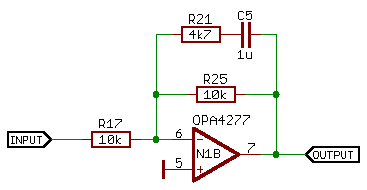
\includegraphics[width=\columnwidth]{graphics/60-hv-amp-dewhitening.pdf}
  \caption[Active inverting dewhitening circuit]{Active inverting dewhitening circuit. This filter uses an inverting op-amp with parallel feedback resistors to achieve the desired frequency response. At low frequencies, the capacitor's impedance is high and so the feedback path is dominated by the impedance of the \SI{10}{\kilo\ohm} resistor and the gain is \num{1}. At high frequencies the capacitor produces very impedance and the feedback path's impedance is the equivalent resistance of the parallel \SI{4.7}{\kilo\ohm} and \SI{10}{\kilo\ohm} resistors and the gain is then $\frac{\SI{10}{\kilo\ohm}}{\SI{3.2}{\kilo\ohm}} \approx \SI{-10}{\deci\bel}$.}
  \label{fig:hv-amp-dewhitening-circuit}
\end{figure}

\begin{figure}
  \centering
  \includegraphics[width=\columnwidth]{graphics/generated/from-python/60-hv-amp-dewhitening-sims.pdf}
  \caption[Simulated dewhitening filter frequency response]{Frequency response of the dewhitening filters simulated with \gls{LISO}. Each dewhitening filter provides \SI{-10}{\deci\bel} gain at high frequencies and so the combined pair produces an overall high frequency gain of $\SI{-20}{\deci\bel} \approx \num{e-1}$.}
  \label{fig:hv-amp-dewhitening-sims}
\end{figure}

\subsubsection{Digital switching electronics}
A series of digital outputs from \gls{CDS} can be used to control the \gls{HV} amplifier's dewhitening filters. The Contec DO-32L-PE output card provides a 32 channel binary switch with an equivalent schematic shown in the left side of Figure\,\ref{fig:hv-amp-sigital-switching}. The control signal from \gls{CDS} for a particular output is inverted and attaches to the negative input of an optocoupler, which acts as a relay without an electrical connection between the input and output. The positive input is attached to a voltage supply such that a digital output of \num{1} results in a closed circuit once inverted. An output of \num{0} is inverted to \num{1} and so there is no potential difference to close the optocoupler's circuit. The optocoupler's output in turn connects to the base of a transistor which controls current flow between the collector and emitter.

\begin{figure}
  \centering
  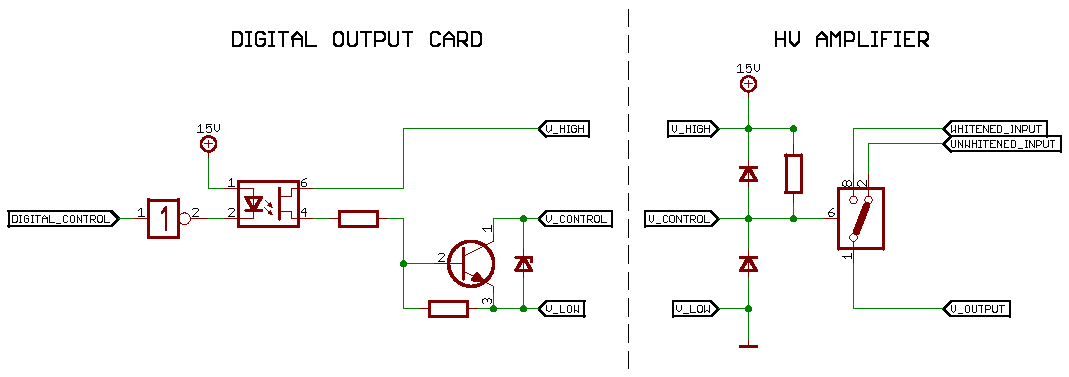
\includegraphics[width=\columnwidth]{graphics/60-hv-amp-digital-switching.pdf}
  \caption[Digital signalling between the control and data acquisition system and a channel within the high voltage amplifier]{\label{fig:hv-amp-sigital-switching}Digital signalling between \gls{CDS} and a channel within the \gls{HV} amplifier. The digital control signal operates an optocoupler which allows current to flow from the $V_{\text{HIGH}}$ voltage reference to a transistor which operates the analogue control signal $V_{\text{CONTROL}}$. This signal is used by the \gls{CMOS} switch in the \gls{HV} amplifier to select either the dewhitened or non-dewhitened signals.}
\end{figure}

The analogue input to the \gls{HV} amplifier for a particular channel is split into two with one passed through the dewhitening filter and the other unperturbed. These two signals form the poles of a \emph{complementary metal-oxide semiconductor} (\gls{CMOS}) switch, chosen for its switching speed, controlled by the digital signal which connects to one of the digital outputs of the \gls{CDS} card via a shielded transmission line. Due to the operation of the digital output card the dewhitening filter control signal $V_{\text{CONTROL}}$ must nominally be $V_{\text{HIGH}}$ which is achieved through the use of a pull-up resistor. When dewhitening is desired, an output of \num{1} at the optocoupler results in a low-resistance path between the control signal and ground and so the control signal within the amplifier becomes $V_{\text{LOW}}$. A truth table is shown in Table\,\ref{tab:digital-dewhitening-truth-table}.

\begin{table}
  \centering
  {\renewcommand{\arraystretch}{1.2} % for extra vertical spacing between rows
    \begin{tabular}{c|c|c}
      \textbf{\gls{CDS} software logic level} & \textbf{$V_{\text{CONTROL}}$} & \textbf{Dewhitening status} \\
      \hline
      0 & $V_{\text{HIGH}}$ & On \\
      1 & $V_{\text{LOW}}$ & Off
    \end{tabular}
  }
  \caption[Truth table for digital switching of dewhitening filters in the high voltage amplifier]{\label{tab:digital-dewhitening-truth-table}Truth table for digital switching of dewhitening filters in the \gls{HV} amplifier, showing the effect that a software logic level in \gls{CDS} has on the dewhitening of the input signal for a particular channel in the \gls{HV} amplifier.}
\end{table}

The electronics shown in Figure\,\ref{fig:hv-amp-sigital-switching} are for a single dewhitener. This configuration must be repeated twice for each of the amplifier's channels to control each of the dewhitening filters.

\subsection{Choice of high voltage op-amp}
Due to the nature of the load the amplifier does not need to drive a significant current, but the voltage noise it produces must be significantly lower than the displacement requirement for the experiment in order for it not to limit its sensitivity. The lowest noise high voltage amplifier integrated circuits available tend to be \gls{MOSFET}-type op-amps. The choice of device tends to be motivated by the bandwidth, maximum output voltage and noise of each particular model.

The \emph{gain-bandwidth product} specifies an op-amp's open-loop gain as a function of the bandwidth it is able to provide it over, and this figure is derived from the speed at which the op-amp's output is able to react to a change in its input (its \emph{slew rate}). The full output voltage is not provided at the unity gain frequency and so a more useful figure of merit is the bandwidth over which the maximum output can be provided. For the \SSMEXPT{} it is expected that radiation pressure and thermal noise will require fast corrections in the \SI{}{\kilo\hertz} range, and to avoid becoming limited by the device's slew rate at higher frequencies (which appears as phase lag on a plot of the frequency response) it is reasonable to require a bandwidth of at least \SI{20}{\kilo\hertz}.

The required \gls{DC} op-amp gain should be known ahead of time in order to fully estimate the effect an op-amp's noise will have on the experiment. The maximum \gls{CDS} input voltage is \SI{\pm10}{\volt} and so to achieve the maximum output voltage requirement when the \gls{CDS} voltage is maximum, thus giving the greatest dynamic range, the op-amp's gain should be set to around \num{40}. From this we can estimate the output noise of some op-amps and determine the Johnson-Nyquist noise (see Section\,\ref{sec:johnson-nyquist-noise}) contribution of the resistors that define the op-amp's \gls{DC} gain.

Table\,\ref{tab:hv-op-amp-comparison} shows the aforementioned parameters for some popular op-amp models. The models shown have sufficient output voltage and identical input noise. The PA89's bandwidth is limited and the full output voltage is not available beyond \SI{7}{\kilo\hertz}, whilst the quiescent power in the PA94 and PA98 is high enough to warrant challenging heat sink requirements. In this case the optimal choice of op-amp is the PA95, for which only a passive heat sink will be required.

\begin{table}
  \centering
  \begin{tabular}{r|c|c|c|c}
    & \textbf{PA89} & \textbf{PA94} & \textbf{PA95} & \textbf{PA98} \\
    \hline
    \textbf{Maximum output} & \SI{1140}{\volt} & \multicolumn{2}{c}{\SI{900}{\volt}} & \SI{450}{\volt} \\
    \textbf{Bandwidth @ \SI{400}{\volt} output} & \SI{7}{\kilo\hertz} & \SI{90}{\kilo\hertz} & \SI{30}{\kilo\hertz} & \SI{60}{\kilo\hertz} \\
    \textbf{Input noise @ \SI{100}{\hertz}} & \multicolumn{4}{c}{\SI{6}{\nano\volt\per\sqrthz}} \\
    \textbf{Quiescent power @ \SI{\pm400}{\volt}} & \SI{3.8}{\watt} & \SI{14.1}{\watt} & \SI{1.3}{\watt} & \SI{17.5}{\watt}
  \end{tabular}
  \caption[Performance specifications for various high voltage operational amplifiers]{\label{tab:hv-op-amp-comparison}Performance specifications for various \gls{HV} op-amps. All of the models listed are manufactured by Apex and the values have been obtained from their respective data sheets. The PA95 was selected due to its low quiescent power for the desired voltage range, which in turn eases the requirement for heat sinking, and the bandwidth is sufficient for the \SSMEXPT{}.}
\end{table}

\subsection{Amplifier signal path}
The amplifier signal path is shown for a single channel in Figure\,\ref{fig:hv-amp-signal-path}. The differential inputs IN+ and IN- are converted to a single-ended signal which is then passed through the two dewhitening stages controlled by digital switches. The signal is then split into two parts, with one part being inverted, before they are input to the PA95 power op-amps. The inputs are clamped together by diodes to ensure that the difference is less than \SI{0.7}{\volt}. This is to prevent the expensive op-amps from damage caused by overvoltage at the inputs, and does not limit the bandwidth or dynamic range in this application. A \SI{1}{\percent} voltage divider at each of the differential outputs provides a signal that is within the input range of \gls{CDS} for the purpose of output monitoring. This provides a readback channel for the controller in order to assist with the calibration of the device.

\begin{figure}
  \centering
  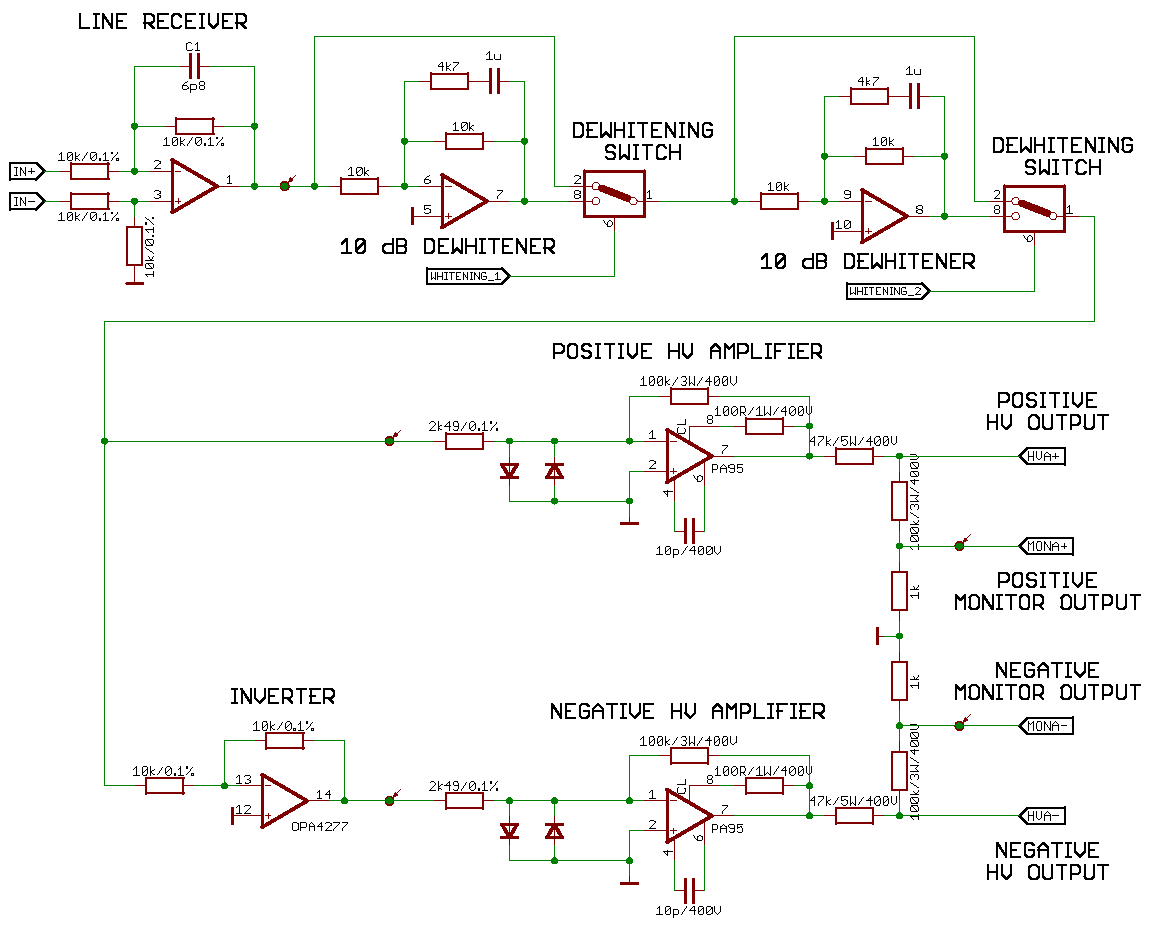
\includegraphics[width=\columnwidth]{graphics/60-hv-amp-signal-path.pdf}
  \caption[High voltage amplifier signal schematic]{\label{fig:hv-amp-signal-path}Schematic of a single high voltage amplifier channel. The input from \gls{CDS} is differentially received, dewhitened and then split into differential outputs that are amplified by PA95 op-amps. A pickoff reads \SI{1}{\percent} of the output voltage for the purposes of calibration.}
\end{figure}

\subsection{Practical and safety features}
As the \gls{HV} amplifier handles potentially lethal current and voltage, a number of additional features beyond the signal circuitry are present.

\subsubsection{Current limiting}
At the output of each \gls{HV} rail there are \SI{47}{\kilo\ohm} resistors which passively limit the current on each rail to around \SI{10}{\milli\ampere}. This operates in addition to an active current limit set via a \SI{100}{\ohm} witness resistor between two pins of each PA95 op-amp. The current limit does not impact the driving of capacitive loads, but ensures that the current produced by the \gls{HV} amplifier is not lethal.

\subsubsection{Soft-start}
Capacitors are present upon the \gls{HV} supply lines to filter \gls{AC} noise, and these must be charged when the device is switched on. Normally these capacitors would present very little impedance to the power supplies and so a large initial current would be drawn, potentially damaging components in its path. The simplest technique to prevent this from happening would be to put resistors in the path of the power supplies, but resistors that would charge the capacitors at a safe rate in a short time would also dissipate a lot of power and require heat sinking. Instead, we use a \emph{soft-start} mechanism which controls the current flow during the charging of the capacitors. The \gls{HV} amplifier's on-off switch operates some optocouplers which allow current to flow into the circuit. Initially, when the circuit's \gls{HV} capacitors are discharged the current on each \gls{HV} rail is limited by the parallel \SI{5}{\kilo\ohm} resistors. A \SI{2.5}{\percent} pick-off from each \gls{HV} rail is compared to a reference \SI{5}{\volt} voltage at an op-amp, the output of which operates a second optocoupler on each rail. When the voltage surpasses \SI{200}{\volt} the power the \SI{5}{\kilo\ohm} resistors dissipate is \SI{8}{\watt}, which is near the reasonable limit for passively cooled resistors. At this point, the capacitors are almost fully charged and the pick-off voltage surpasses the \SI{5}{\volt} reference, and so the op-amp's output operates the optocoupler to open up a low-resistance path that bypasses the \SI{5}{\kilo\ohm} resistors and prevents them from overheating. This is shown in Figure\,\ref{fig:hv-amp-soft-start}.

\begin{figure}
  \centering
  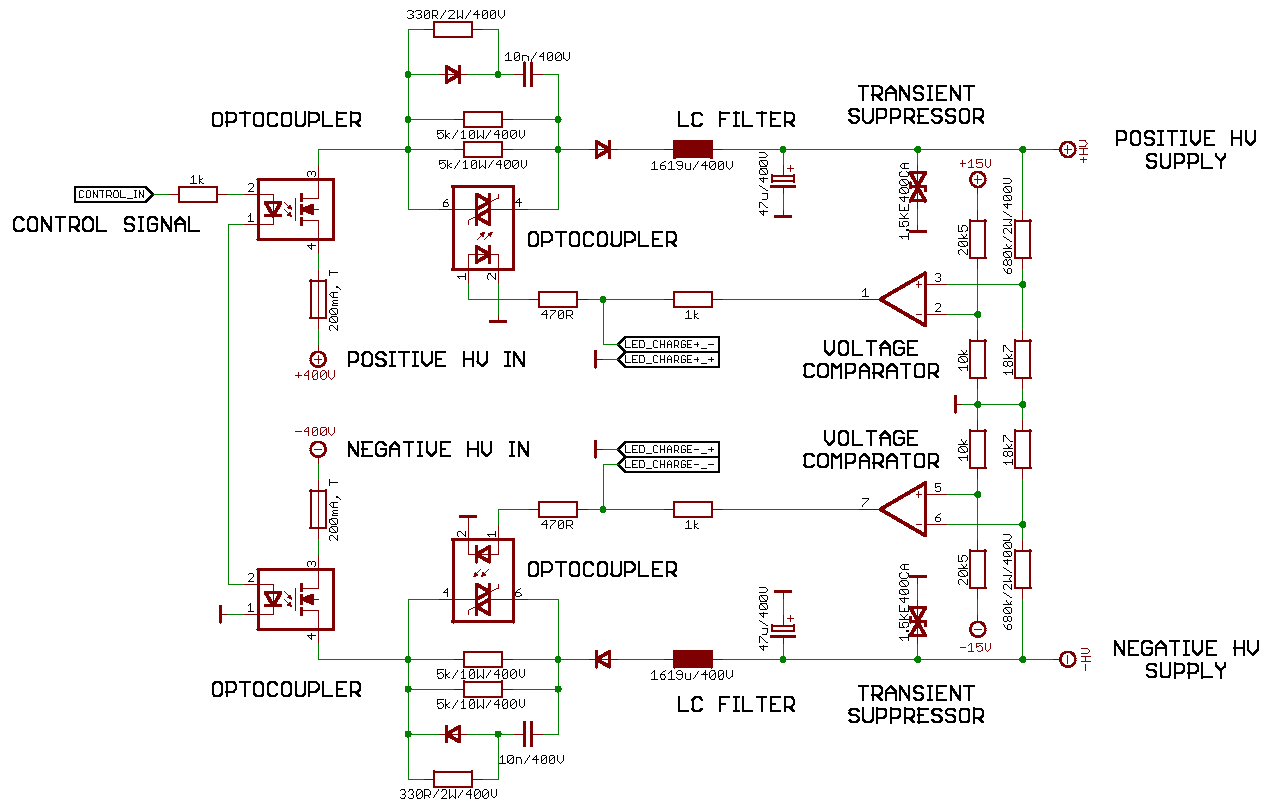
\includegraphics[width=\columnwidth]{graphics/60-hv-amp-soft-start.pdf}
  \caption[High voltage amplifier soft-start schematic]{\label{fig:hv-amp-soft-start}Soft-start mechanism to prevent excessive power supply current draw. This design is based on one the soft-start mechanism for a device produced for the \AEIPROTOTYPE{} by Andreas Weidner. The leftmost optocouplers control whether current is allowed to flow from the power supplies given a control signal from an on-off switch on the enclosure. After the electronics are switched on, the current flow is initially limited by two \SI{5}{\kilo\ohm} resistors. Any \gls{AC} signal content is filtered by the presence of a \SI{1.6}{\milli\farad} choke. A \SI{2.5}{\percent} pick-off from each \gls{HV} rail is compared to a \SI{\pm5}{\volt} reference, with the resulting difference fed back to a second pair of optocouplers which gradually open up a low-resistance path on each supply rail. Without these optocouplers, the power the \SI{5}{\kilo\ohm} resistors would need to dissipate would be considerable at maximum voltage. As the supply voltage increases beyond around \SI{200}{\volt}, the resistance through the optocoupler is reduced far below the \SI{5}{\kilo\ohm} resistors and so the power dissipated in the resistors is negligible.}
\end{figure}

\subsubsection{Pressure and temperature interlock}
The breakdown voltage of the plate capacitors as a function of pressure, given by Paschen's Law, has a minimum in the region of \SI{e-1}{\milli\bar} to \SI{e1}{\milli\bar} depending on the separation and geometry of the anode and cathode, as shown in Figure\,\ref{fig:esd-paschen}. In addition, related effects such as surface tracking can lead to arcing at voltages above \SI{50}{\volt} in low vacuum.

Although the use of high voltage plate capacitors is in general safe at both atmospheric pressure and high vacuum, the act of pumping gas out of the vacuum system necessarily passes through pressures at which arcing can occur. To prevent the possibility of arcing, a cut-off function is present within the circuit to prevent high voltage output unless a control signal is supplied (see Figure\,\ref{fig:hv-amp-interlock}). This signal will be produced by \gls{CDS} derived from a separate pressure monitor. Additionally, as a temperature fail-safe for the amplifier components, temperature sensors are present within the enclosure which operate threshold switches able to remove the supply current via the same mechanism as the pressure interlock. The outputs from each interlock are sent to an AND gate. Only if both the pressure and temperature switches are switched on will the control signal used to operate the \gls{HV} supplies switch on. The interlock circuit is shown in Figure\,\ref{fig:hv-amp-interlock}.
% pressure vs voltage claim from speedmeter labbook, at https://arran.physics.gla.ac.uk/wp/speedmeter/2015/01/30/esd-hv-amplifier-pressure-cutoff/

\begin{figure}
  \centering
  \includegraphics[width=\columnwidth]{graphics/generated/from-python/60-esd-paschen.pdf}
  \caption[Minimum breakdown voltage between the two plates of the electrostatic drive for different separations]{\label{fig:esd-paschen}The minimum breakdown voltage between the two plates of the \gls{ESD} for different separations. This is calculated using Paschen's Law, assuming nitrogen gas and a flat plate geometry. The real effect is a lot more complicated than this model, but the steep slope at lower pressures shown here indicates that the voltage created by the \gls{HV} amplifier for the \gls{ESD} experiment will avoid problems associated with arcing as long as it is operated at atmosphere or high vacuum.}
\end{figure}

\begin{figure}
  \centering
  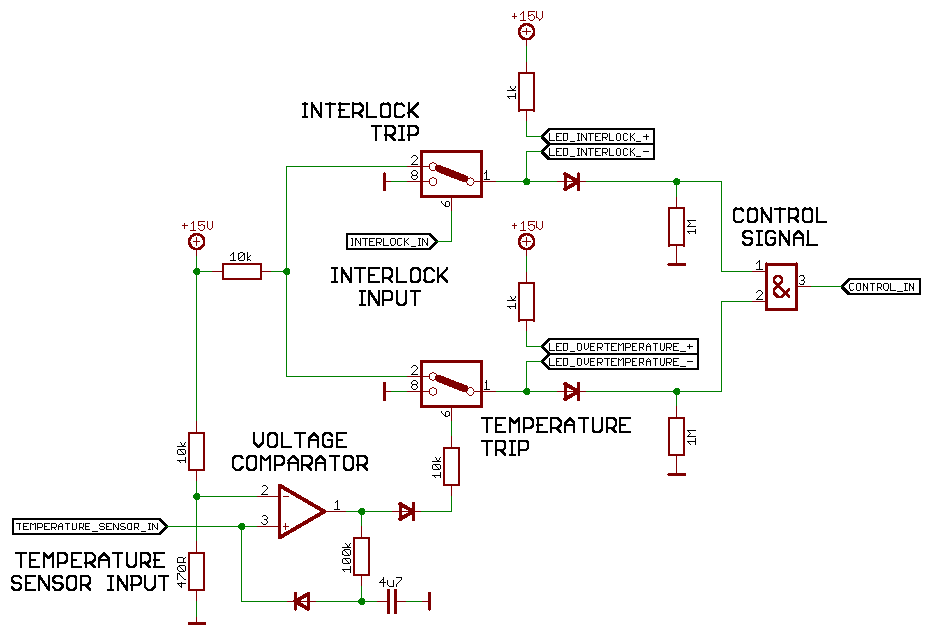
\includegraphics[width=\columnwidth]{graphics/60-hv-amp-interlock.pdf}
  \caption[High voltage amplifier interlock schematic]{\label{fig:hv-amp-interlock}Pressure and temperature interlock circuit. The digital interlock signal from \gls{CDS} operates one switch and the output from a temperature sensor threshold switch operates another. Only if both switches output \SI{15}{\volt} will the control signal used to operate the \gls{HV} supplies switch on.}
\end{figure}

\subsection{Transfer functions and noise measurements}
Transfer functions for the \gls{HV} amplifier can be measured by injecting a known signal into one channel and measuring the corresponding output. The monitor output provides a means of measuring \SI{1}{\percent} of the full \gls{HV} output with a signal that is within the input range of \gls{CDS}.

\subsubsection{Swept sine response of each channel}
Figure\,\ref{fig:hv-amp-dewhitened-tfs} shows the \emph{swept sine} response, calculated by injecting a sine wave at a given frequency, measuring the output signal and dividing it by the injection. These measurements were made without the digital dewhitening switches engaged such that they provide \SI{20}{\deci\bel} of low-pass filtering. The figure shows the response expected from the predictions made by \gls{LISO} shown in Figure\,\ref{fig:hv-amp-dewhitening-sims}.

\begin{figure}
  \centering
  \includegraphics[width=\columnwidth]{graphics/generated/from-python/60-hv-amp-dewhitened-tfs.pdf}
  \caption[Frequency response of the high voltage amplifier's channels with dewhitening enabled]{Second amplifier transfer functions with dewhitening enabled. The expected performance of the dewhitening filter from theory is shown in \checkme{purple} alongside the transfer functions of each channel. The curves agree closely, showing that the implemented filter operates as expected. The mismatch at high frequency is caused by the anti-aliasing filters implemented in \gls{CDS}, which aggressively filter signals above a few \SI{}{\kilo\hertz}.}
  \label{fig:hv-amp-dewhitened-tfs}
\end{figure}

\subsubsection{Response with and without dewhitening}
Figure\,\ref{fig:hv-amp-channel-one-tfs} shows swept sine measurements of the first channel with the dewhitening filters in various states: both on, the first on and the second off, the first off and the second on, and both off. The measurements match predictions and the response with both dewhiteners off is flat as intended across the measurement band.

\begin{figure}
  \centering
  \includegraphics[width=\columnwidth]{graphics/generated/from-python/60-hv-amp-channel-one-tfs.pdf}
  \caption[Transfer functions of the high voltage amplifier input to monitor output with the dewhiteners on and off]{Transfer functions of the high voltage amplifier input to monitor output with the dewhitening filters on and off. The monitor output is a \SI{1}{\percent} pick-off from the main \gls{HV} output, and so the gain is \num{0.4} instead of \num{40}. The curves simulated with \gls{LISO} agree exactly with the measurements within the bandwidth of \gls{CDS}, and beyond around \SI{3}{\kilo\hertz} the transfer functions are suppressed by the anti-aliasing filters on \gls{CDS}'s \glspl{ADC}.}
  \label{fig:hv-amp-channel-one-tfs}
\end{figure}

\subsubsection{Coherence between channels}
The channels should be isolated from one another such that a signal injected at one input does not appear at the output of another. Power supply filtering is implemented using capacitors, inductors and diodes such that there should be minimal cross-coupling between the channels. Figure\,\ref{fig:hv-amp-coherence} shows the coherence for each channel to each other channel, measuring whether the output signal has the same phase angle as the input signal. Coherence of \num{1} indicates that there is causal coupling between the two channels, whereas coherence less than around \num{0.5} is expected from statistical random noise processes. This confirms that a high level of isolation between channels is achieved.

\begin{figure}
  \centering
  \includegraphics[width=\columnwidth]{graphics/generated/from-python/60-hv-amp-coherence.pdf}
  \caption[High voltage amplifier cross-channel coherence]{\gls{HV} amplifier cross-channel normalised coherence. A swept sine was injected into each channel in turn whilst measurements of the output phase were made on all four channels. In each case, only the channel with the injection has coherence of \num{1}, while other channels only show the effect from noise.}
  \label{fig:hv-amp-coherence}
\end{figure}

\subsubsection{Output noise}
\note{Show noise projected into effective test mass displacement, and show how this is smaller than the requirement}

% No data yet
% \section{Experimental test of the electrostatic drive}
% To set requirements on the positioning of the plates, and to build and test the infrastructure for the operation of the \glspl{ESD}, this chapter introduces the design for an experiment to test the new \gls{ESD} design.
% 
% \begin{table}
%   \centering
%   \begin{tabular}{ll}
%     \textbf{Parameter}   & \textbf{Value} \\
%     Mirror diameter      & \SI{30}{\milli\meter} \\
%     Mirror thickness     & \SI{6}{\milli\meter} \\
%     Single plate width   & \SI{30}{\milli\meter} \\
%     Single plate length  & \SI{50}{\milli\meter} \\
%     Nominal plate separation & \SI{40}{\milli\meter} \\
%   \end{tabular}
%   \caption[Plate capacitor and optic parameters for the experiment to test the electrostatic drives for the \SSM{}]{\label{tab:esd-expt-parameters}Plate capacitor and optic parameters for the experiment to test the electrostatic drives for the \SSM{}.}
% \end{table}
% 
% Although the \gls{ESD}, and indeed the \SSM{} experiment, primarily require corrections at lower frequencies where seismic noise is dominant, it is beneficial to utilise an amplifier which can provide actuation up to many tens, if not hundreds, of \SI{}{\kilo\hertz}. This facilitates a transfer function which is flat across the vast majority of each experiment's measurement band, avoiding the roll-off at high frequencies due to the integrated circuits utilised within the high voltage amplifier. A flat transfer function makes the calibration of the actuator plant as part of the overall experiment as simple as possible. Another benefit of having a high bandwidth amplifier is the possibility to use it for common mode control loops, where laser frequency stabilisation can be split between feedback to the laser's piezoelectric transducer and actuators on the test masses.
% 
% The key component of a high bandwidth amplifier is the power op-amp. This class of op-amps typically utilises a \gls{MOSFET} design, and can provide high voltage output given a low voltage input. As an example, the Apex PA95 op-amps used in Advanced LIGO's \glspl{ESD} provide up to \SI{900}{\volt} output up to a frequency of around \SI{15}{\kilo\hertz}, and up to \SI{50}{\volt} at \SI{250}{\kilo\hertz}. The PA98 op-amp, also from Apex, provides an output of \SI{450}{\volt} nominally up to \SI{60}{\kilo\hertz}, potentially up to \SI{500}{\kilo\hertz} for a low capacitive load. For the purposes of this experiment, the choice was made to use the PA98 op-amp to provide the ability to study the effect of the actuator across a very wide bandwidth. To this end, an amplifier circuit utilising the PA98 was built based on a design used for the \AEIPROTOTYPE{}. This design provides up to \SI{\pm350}{\volt} output, and originates from a single-ended, \SI{350}{\volt} amplifier design where the PA98 is especially suited. Two notable modifications have been made, with a view to safety.
% 
% % claim about voltage output of PA95 comes from figure ``Power Response'' on p3 of PA95 datasheet (https://www.apexanalog.com/resources/products/pa95u.pdf)
% % claim about voltage output of PA98 comes from figure 8: ``power Response'' on p7 of PA98 datasheet (https://www.apexanalog.com/resources/products/pa98u.pdf)

\section{Outlook}
Parallel plate capacitor \glspl{ESD} provide a low noise alternative to voice coil actuators for the control of suspended test masses, and it is intended for \glspl{ESD} to be used as the high frequency actuators in the \SSMEXPT{}. In order to provide actuation at the required level, an \gls{HV} signal must be supplied to each \gls{ESD}. The technical design of a \gls{HV} amplifier was presented with the intention to provide actuation at the required level and with low enough noise to meet the requirements of the experiment, and measurements show that the design meets the requirements.
\chapter{Integration of slow control channels in LIGO CDS}
\label{c:slow-controls-integration}

\section{Motivation and Requirements}
Context, motivation, requirements...

Channel list, graph diagram (graphviz?) of signal pathways?

\section{The LIGO CDS system}
The \gls{CDS} system designed for use in \gls{LIGO} and used for the practical experiments in Chapters \note{X, Y, Z} provides high-speed, low-noise analogue-to-digital and digital-to-analogue converters (\glspl{ADC} and \glspl{DAC}, respectively) to send signals between the experimental hardware and the software-defined controls. The software-defined controls run within a real-time Linux kernel, allowing for deterministic operation, and the channel infrastructure is built on top of the widely used open-source \emph{\gls{EPICS}} system. While \gls{CDS}'s inputs and outputs are well suited to the measurement and control of key sensors and actuators within a low-noise experiment, they are also expensive. Each input or output channel consists of various integrated circuits and filters, all of which must be carefully chosen to minimise noise which can potentially contaminate the sensitivity of the system, along with power supply components, specialised connectors and rack infrastructure; this leads to an expense per channel of roughly \checkme{\pounds600}.

\section{EPICS and CDS}
Industrial-style control is not uncommon in large physics experiments such as \gls{LIGO}. Originally designed for the Advanced Photon Source particle physics experiment at Argonne National Laboratory, Chicago, USA, the \gls{EPICS} system provides the ability to define an arbitrary number of channels for the purposes of control. The \gls{CDS} system uses \gls{EPICS} to handle its control infrastructure.

\subsection{Input/output controllers}
One of the key advantages of this system is that the channels may be defined across any number of separate input/output controllers (\glspl{IOC}), which may be on separate, remote servers. This is useful from the point of view of large experiments, where to minimise transmission noise pick-up (see \ref{sec:signal-and-noise-paths}) controllers are situated close to devices to be controlled. At the Advanced LIGO facilities, for example, the end stations are separated from the main building by \SI{4}{\kilo\meter}, and so transmission noise to and from the main building would be significant. Instead, \glspl{IOC} are present within each end station, communicating with the master control system in the main building via a fibre optic network.

\subsubsection{Channel access via EPICS}
The distributed nature of \gls{EPICS} requires a network protocol capable of both determining the location of a particular channel on a particular \gls{IOC}, and reading its data in a timely manner. For this aspect \gls{EPICS} provides the \emph{channel access} (\gls{CA}) network protocol. When a particular channel is desired by a host, the \gls{CA} protocol issues a multicast packet to the local network to ask for the location of that channel. The \gls{IOC} associated with the channel, upon receiving this request, will respond with a message to say that it has the channel. Finally, the \gls{CA} protocol will send or receive data to the channel via the respective \gls{IOC} as required.

Channels are accessed by combining a \emph{host} and local channel name in the form \lstinline!HOST:CHANNEL!. The host need not necessarily be the name of the physical server hosting the channel's \gls{EPICS} \gls{IOC}, but rather a logical group. In Advanced LIGO, for example, the host is specified as the interferometer associated with each channel: \lstinline!H1! and \lstinline!L1! for the Hanford and Louisiana sites, respectively. In this way, channels may be moved from one \gls{IOC} to another without having to update control infrastructure that utilises such channels.

\subsection{Frame builder}
Recorded channels are read from \gls{EPICS} by the \gls{CDS} \emph{frame builder}. This is a software service which compiles individual files containing \SI{16}{\second} data chunks in the \gls{LSC}-standard gravitational-wave frame (\gls{GWF}) format. This system runs in real time, with signals received via \gls{CDS} channels recorded deterministically. The frame builder can also record other EPICS channels not necessarily associated with \gls{CDS} inputs or outputs. This is useful to record information about auxiliary control information. In the \gls{CDS} control system, for example, a \emph{filter bank} is typically used to apply low- or high-pass filters and offsets to output signals. The values associated with these filters and offsets are contained in EPICS channels and can thus be stored in frames.

\subsubsection{Data acquisition}
Large \gls{CDS} experiments with many filter banks and complex control systems possess many \gls{EPICS} channels. In Advanced LIGO, the total number is of the order \num{200000} \cite{aligonoise2016}. Even in a lab-based experiment the number can grow to many thousands. Hardware limitations prevent every channel from being recorded at the highest possible speed: hard drive storage and \gls{CPU} speed would quickly become saturated. Instead, the frame builder allows channels to be acquired at a specific sample rate, or not at all. This allows channels containing useful high frequency signals to be recorded at a sample rate allowing the underlying signal to be recovered, while recording low frequency signal channels at a rate which doesn't waste storage space.

\subsection{The Glasgow CDS system}
In the laboratory housing the \GLASGOWTENM{} and \SSM{} experiments, a control room is separated from the clean room. The \gls{CDS} system is used for experimental control, with the main frame builder situated in the control room. Separate so-called \emph{front-ends} are situated in the control room and the clean room, providing analogue and digital interfaces to the experiment to allow signals to be sent to and from the frame builder.

\section{Monitoring auxiliary channels}
The monitoring of environmental variables such as ambient temperature and pressure does not necessarily require the expensive, low noise channels provided by \gls{CDS}. Even for the largest of experiments, for example Advanced LIGO, the \gls{CDS} system is run in parallel with a different system using cheaper hardware, for the purposes of monitoring such auxiliary data streams. For the \SSMEXPT{}, the choice was made to utilise hardware running the \emph{EtherCAT} system. This uses standard Ethernet network cable to transport analogue and digital signals between hardware termini. Differential signalling is also a feature, which allows for transmission noise pick-up to be minimised (see \ref{sec:signal-and-noise-paths}).

It is desirable to be able to combine the \emph{slow} channels monitored by EtherCAT with the \emph{fast} channels and real-time control system provided by \gls{CDS}.

\section{Slow controls with CDS}
As the \gls{CDS} frame builder is capable of recording any \gls{EPICS} channels, it is desirable to integrate EtherCAT channels into \gls{EPICS}. An added benefit of this approach is that, having \gls{EPICS} analogues, EtherCAT channels may be integrated into the same control loops as the main experiment's fast channels, albeit at a much slower rate.

\subsection{Polling rate and aliasing}
The frame builder cannot reliably record data from remote \glspl{IOC} at high data rates, and so it is limited to \SI{16}{\hertz}. This can be checked with a simple experiment. With an \gls{IOC} running on a remote machine, the frame builder can be asked to acquire a channel on the remote \gls{IOC} into which a known signal is injected. A new \gls{IOC} was configured (\lstinline!cds-fe3!) with an analogue input channel \lstinline!G2:TEST-test_input_1! (``G2'' is the name given to the Glasgow site). A discrete sine wave was generated programmatically in the form:
\begin{equation}
  \label{eq:programmatic-sine}
  A_{i} = A_0 sin \left( 2 \pi f t_{i} \right)
\end{equation}
where $A_{i}$ represents the $\text{i}^{\text{th}}$ output, $A_0$ is the amplitude, $f$ is the signal frequency and $t_{i}$ is the $\text{i}^{\text{th}}$ time step. The time steps are determined via the sample rate $f_{\text{s}}$:
\begin{equation}
  \label{eq:programmatic-time-step}
  t_{\text{i}} = t_{\text{i}-1} + \frac{1}{f_{\text{s}}}
\end{equation}
With the definition that $t_{0} = 0$, the above equations can be used to generate an arbitrary signal at an arbitrary sample rate, within system performance constraints.

Equations\,\ref{eq:programmatic-sine} and \ref{eq:programmatic-time-step} were implemented in Python alongside an \gls{EPICS} communication library. Channel \lstinline!G2:TEST-test_input_1! was injected with the sine wave over \num{5} cycles and was simultaneously acquired by the frame builder. The same signals sent to the frame builder were recorded locally. The test configuration is shown in Figure\,\ref{fig:epics-ioc-test}. Figure\,\ref{fig:epics-test} shows a sine wave with amplitude \num{1000}, frequency \SI{0.1}{\hertz} and sample rate \SI{32}{\hertz} recorded both locally and via the frame builder. The signal recorded locally is recovered by the frame builder, though with an offset of approximately \SI{1}{\second} (not shown). To demonstrate the difference in sample rate, Figure\,\ref{fig:epics-test-stars} shows the discrete data points that form the first peak of the sine wave. Here it is possible to see that the \SI{32}{\hertz} signal recorded by the frame builder across the network is sampled at \SI{16}{\hertz}, witnessed from the presence of \checkme{two blue markers for every one orange marker}.

\begin{figure}
  \centering
  \includegraphics[width=\columnwidth]{graphics/generated/from-svg/70-epics-ioc-test.pdf}
  \caption{\label{fig:epics-ioc-test}Configuration for EPICS IOC test. A Python program running on \lstinline!cds-fe3! generates a sine wave and injects it into the EPICS IOC running on the same machine. The frame builder running on \lstinline!cds-fb1! is able to communicate with the EPICS IOC on \lstinline!cds-fe3! using the Ethernet network.}
\end{figure}

\begin{figure}
  \centering
  \includegraphics[width=\columnwidth]{graphics/generated/from-python/70-epics-test.pdf}
  \caption{\label{fig:epics-test}Test of EPICS recording from a remote IOC. The sine wave recorded locally is recovered remotely by the frame builder. Note that an offset has been applied to the remote data to synchronise the start points: in reality, there exists a timing latency between the local and remote signals.}
\end{figure}

\begin{figure}
  \centering
  \includegraphics[width=\columnwidth]{graphics/generated/from-python/70-epics-test-stars.pdf}
  \caption{\label{fig:epics-test-stars}The first peak of the sine wave presented in Figure\,\ref{fig:epics-test}. The sine wave generated at a sample rate of \SI{32}{\hertz} is recorded locally at that frequency, whereas the data recorded by the frame builder across the network is at half that rate, \SI{16}{\hertz}, shown by the presence of \checkme{two blue markers for every one orange marker}.}
\end{figure}

\subsection{Maximum realistic measurement frequency}
The effect of the sample rate can be further witnessed in Figure\,\ref{fig:sample-aliasing}, where a signal with frequency \SI{8}{\hertz} is generated with sample rate \SI{128}{\hertz}. The frame builder is just able to reconstruct the waveform by sampling the underlying signal at various points in its evolution, which is only possible because the signal has a frequency half the frame builder's sample rate. From the Nyquist-Shannon sampling theorem, the fidelity of a numerical representation of a signal at frequency $f$ is maintained if and only if the sample rate is at least $2f$. If the signal were to be at a higher frequency, the frame builder would be unable to fully reconstruct the signal and instead higher frequency signal content would appear as lower frequency aliasing. This sets the upper frequency limit to signals on external \gls{EPICS} \glspl{IOC} that can be sensed with the frame builder.

\begin{figure}
  \centering
  \includegraphics[width=\columnwidth]{graphics/generated/from-python/70-epics-aliasing.pdf}
  \caption{\label{fig:sample-aliasing}The frame builder's sample limit. With a signal of frequency \SI{8}{\hertz}, the frame builder, sampling at a rate of \SI{16}{\hertz}, is just able to interpret the underlying waveform. Note the slight drift in the sampling phase, which probably arises from non-deterministic networking and computational interrupts. Signals above \SI{16}{\hertz} will appear aliased when measured by the frame builder. Note that, as with Figure\,\ref{fig:epics-test}, a timing latency between the two waveforms has been removed for clarity.}
\end{figure}

\subsection{Timing drift}
Show glitches caused by mismatch in sampling frequencies...

Show FFT with ripples

\begin{figure}
  \centering
  \includegraphics[width=\columnwidth]{graphics/generated/from-svg/70-epics-drift.pdf}
  \caption{\label{fig:epics-drift}Drift of measurements made by frame builder compared to samples generated by Python. Despite intending to produce samples at the same rate that the frame builder takes measurements, drift due to program execution gradually accumulates. Eventually, the frame builder measures the same point twice (in this example, point 8), which is what we see as a ``glitch''. With a particular lab computer the delay accumulation rate was determined to be \SI{6}{\milli\second\per\second}.}
\end{figure}
% 6 ms/s figure from https://arran.physics.gla.ac.uk/wp/speedmeter/?p=8662

Show no glitches when threading is used to prevent wait time between samples...

The delay per cycle for the lab computer is:
\begin{equation}
  t_{\text{delay, cycle}} = f_{\text{s}} \frac{\delta t_{\text{delay}}}{\delta t}.
\end{equation}
If we assume that the program execution time is identical in both threaded and non-threaded cases, this technique will work for frequencies up to the inverse of the delay per cycle, $f_{\text{max}} = \frac{1}{t_{\text{delay, cycle}}} = \SI{2.6}{\kilo\hertz}$. This falls well within the specification of the slow controls system.

\section{Interfacing EtherCAT to EPICS}
With the connection made between remote \gls{EPICS} \glspl{IOC} and \gls{CDS} defined, the remaining step is to provide a means of transferring signals between EtherCAT devices and \gls{EPICS}. As with \gls{EPICS} itself, the scientific community at large has overcome this problem in the form of \emph{dls-ethercat} module developed for the Diamond Light Source synchrotron facility in Oxfordshire, UK.

\subsection{EtherCAT to EPICS}

\subsection{Throughput tests}

\subsection{Integration with CDS controls}

\subsection{Combined slow and fast controls}
\note{Tests...}
\chapter{\label{c:et-lf-control}Control of the low frequency Einstein Telescope detector}

\begin{itemize}
  \item Build upon the PDH stuff laid out in Chapter 3: describe the evolution of the ET-LF interferometer in order to control it: the need for a Schnupp asymmetry (to provide the equivalent of a PDH-style controller), DARM offset, etc...
  
  \item Tobin's talk at G0900745 is really good for explaining DC readout's benefits
  
  \item Talk about the need for an OMC
  
  \item See documentation from ET-LF repository, and aLIGO design study
  
  \item Also see scribblings / emails from Ken etc. around the time of the Florence meeting where we discussed the low frequency sensing problem
  
  \item p255 of design study shows why we need 2 filter cavities for ET-LF and 1 for ET-HF
  
  \item See noise budget from before Florence
  
  \item Show plots of sideband powers not entering the cavities

  \item The Einstein telescope facility: ET-LF and ET-HF, the xylophone, etc.
    \begin{itemize}
      \item Unprecedented LF sensitivity: opens up universe
      \item Pushing warm technology to the limit with ET-HF
      \item Challenges: control at low frequencies with such detuning
      \item ET-LF layout
      \item Predicted sensitivity vs Optickle calculated sensitivity
      \item ISC stuff...
	\begin{itemize}
	  \item Consider only plane waves - justification: only want to control lengths for now. Angles are not considered a challenging aspect as nothing much has changed since aLIGO.
	  \item Optical response: with and without mechanical TFs - show the difference it makes to the response at low frequencies, and why it is necessary to turn them off in the case when you're computing a sensing matrix
	  \item From sensing matrix to control matrix (control loops, locking order, bandwidth, etc.)
	  \item Dynamic range of sensors and actuators in ET-LF
	  \item Problem with dynamic range, need local control or SPI or similar
	\end{itemize}
      \end{itemize}
      
  \item See p5 of VIR-0449D-11 (2011), Advanced Virgo steady state length sensing and control simulation, for description of why DARM offset is better than MICH
\end{itemize}
  
See Bryan's paper for sidebands on sidebands in the context of the Caltech prototype for aLIGO, to describe the use of beats between sidebands: https://iopscience.iop.org/article/10.1088/0264-9381/23/18/010/pdf

\section{The Einstein Telescope Facility}

\subsection{ET-LF}

\subsection{ET-HF}

\section{Control concepts}
\subsection{DC readout}
\subsubsection{Optimal operating point}
In Equation\,\ref{eq:mich-p-out} see that a static field $\frac{P_{\text{in}}}{2}$ is present upon the photodetector, independent of the arm length change. In simple experiments, often it is practical to keep the interferometer at an operating point commonly referred to as ``half way up the fringe''. Here, the interferometer's mirrors are nominally positioned such that the output signal is oscillating about the midpoint between crest and trough (see Figure\,\ref{fig:optimal-operating-point}). As the gradient is steepest at this point, any small changes to the relative arm length of the Michelson interferometer result in a significant difference in power at the photodetector. This operating point, however, is not optimal in terms of \emph{sensitivity} to arm length fluctuations. As discussed in Section\,\ref{sec:snr}, the noise level is just as important as the signal.

%% FIXME: change this plot's x-labels to use wavelength, to fit with the conclusion in the text.
\begin{figure}
  \centering
  \includegraphics[width=\columnwidth]{graphics/generated/from-python/80-optimal-operating-point.pdf}
  \caption[Fringe]{\label{fig:optimal-operating-point}Optimal operating point.}
\end{figure}

By inspecting Equation\,\ref{eq:mich-p-out}, it is clear to see that there must exist, in cases where there is a signal due to a difference in arm length, a static photodetector power independent of the arm length. This does not contribute any displacement information to the measurement, but does contribute shot noise:
\begin{equation}
  P_{\text{shot, out}} = \sqrt{2 h f_0 P_{\text{in}}},
\end{equation}
where $h$ is Planck's constant, $f_0$ is the light frequency and $P_{\text{in}} = A_{\text{in}}^2$, the power entering the interferometer at the beam splitter. The optimally sensitive operating point is therefore not simply one which maximises the signal gradient, but rather one which maximises the SNR. The SNR is:
\begin{equation}
  \text{SNR} = \frac{P_{\text{out}}}{P_{\text{shot, out}}} = \sqrt{\frac{P_{\text{in}}}{4 h f_0}} \left( 1 + \cos \left(k \Delta x \right) \right).
\end{equation}

The $\Delta x$ term in Equation\,\ref{eq:mich-p-out} is a combination of a static arm length \emph{detuning}\textemdash representing the arm length mismatch required to reach the desired operating point\textemdash and a differential gravitational wave signal $\Delta x_{\text{GW}}$. A suitable choice of $ x_{\text{tune}}$ can remove the majority of the static power present at the output. Setting the slope of the SNR with respect to the tuning to zero,
\begin{equation}
  \frac{\Delta \text{SNR}}{\Delta x_{\text{GW}}} = -k \sqrt{\frac{P_{\text{in}}}{4 h f_0}} \sin \left(k \Delta x\right) = 0,
\end{equation}
we find that maximum SNR is achieved for static tunings 
\begin{equation}
  \Delta x \text{ mod } \lambda = 0.
\end{equation}
This result shows that the optimal operating point in terms of SNR is at the point where the light from the two arms interferes destructively. While any multiple of $\lambda$ will satisfy the SNR condition as defined, in reality we have not considered laser noise coupling. The more matched the arm lengths are, the lower the laser noise couples to the output port. In reality there are also mismatches in the reflectivities of the mirrors in the arms: this creates an asymmetry called a \emph{contrast defect} which leads to additional shot noise at the output port.

%CHECKME At the output port, light from one arm is transmitted through the beam splitter while the light from the other arm is reflected, and so a reflection phase convention applies (see Appendix\,\ref{a:reflection-phase}). The arm lengths are therefore offset by $\frac{\lambda}{4}$ with respect to one another.

% Section 1.3.1 of Gabriele Vajente's thesis covers this in more detail.

\subsection{Challenges}
\note{Focus on ET-LF, but discuss challenges with ET-HF too (parametric instabilities, etc.) - basically stress that there's a lot of work to be done before the technical design}

\note{Discuss that we need to model both tuned and detuned ET-LF states, as the locking will have to start with tuned}

\section{Control of an interferometer with multiple degrees of freedom}
\note{Control matrix...}

\section{Modelling ET-LF}
\note{See email sent to Andreas about outcomes of ASPERA. Basically, we had to model the interferometer controls and higher order modes, so we did it simultaneously with two tools. Discuss how this was achieved, via a shared parameter set, etc.}

\begin{figure}
  \centering
  \includegraphics[width=\columnwidth]{graphics/generated/from-svg/80-darm-schnupp-offsets.pdf}
  \caption[Differential arm and Schnupp offsets in a \DRFPMI{}]{\label{fig:darm-schnupp-offsets}Blah}
\end{figure}

\subsection{Modelling higher order modes and parametric instabilities}
\note{Finesse...}

\subsection{Modelling control loops}
\note{Optickle + SimulinkNb}
Optickle facilitates the modelling of control loops in a number of ways. The primary output from an Optickle simulation is the interferometer matrix, describing the mapping of every degree of freedom of the interferometer to every probe within the interferometer. As such, with this matrix it is possible to construct the signals produced by the various readouts within the interferometer, and these can be manually propagated through electronics to calculate the signal characteristics in a controller. Furthermore, Optickle is written in Matlab and so benefits from the \emph{Simulink} and \emph{Control Systems} toolboxes provided as extensions, with which it is possible to define control loops around the interferometer plant and perform linearisation to calculate loop gains and transfer functions. With a little effort, this process can be automated in a script. However, an \gls{LSC} tool developed for \gls{LIGO}, \emph{SimulinkNb}, became available in 2015 and acts as an interface between Optickle and Simulink. It is primarily designed to calculate out-of-loop noise budgets for an interferometer model defined within Optickle, and as a consequence of this it is able to model control loops.

\subsection{Combined modelling effort}
It was decided that the best approach to combine the benefits of the two tools would be to develop identical models with both Finesse and Optickle...

\subsection{Recycling cavity lengths and RF sidebands}
\note{Defined sideband frequencies...}

\note{Discuss how we chose to follow Advanced LIGO as much as possible, but had to define some as-yet undefined parameters first}

\section{Conceptual control scheme}

\note{Put the control matrices here: show the slopes of the error signals for tuned and detuned operation}

\section{Control noise}
\note{Highlight the dynamic range problem with photodetectors sensing the low frequency motion (poster from Florence), and introduce the basic control loop developed with SimulinkNb - discuss the noises included, the assumptions made, etc. Finish with the list from the poster of what has to be done: further modelling of suspension SPIs, or better sensors, or both, etc...}

\subsection{Seismic noise in ET-LF}
\note{Take transfer function through S.A. from lowest noise site measured...}
\note{Assume optimal worst contribution of noise to ETMs...}

\section{Outlook}

\subsection{Future upgrades to ET}
\note{SSM, Stefan D's idea for triangular speed meter, etc...}

% appendices
\appendix
\chapter{\label{a:simulation-tools}Simulation Tools}
How to build simulations in both tools...

\note{Mention about difference in homodyne angles between Optickle and Finesse - empirical formula on speedmeter labbook post from end of 2015/early 2016}

\section{Finesse}

\section{Optickle}
Optickle is a tool primarily designed to produce a series of matrices as outputs. As it is based in \MATLAB, it is possible to study the behaviour of the code to determine its capabilities and limitations. This section attempts to explain the basic operation of the primary feature that Optickle provides: the \lstinline{tickle} function.

In order to simulate an interferometer, an optical environment is created into which optics, sensors and links between optics may be defined. The primary output of Optickle is a transfer matrix mapping \emph{drives} of each optic in the system to probes within that system. A drive is simply a degree of freedom of an optic, such as longitudinal motion of a mirror. Probes are the simulation equivalent of photodetectors, but can be lossless and can perform arbitrary RF demodulations. Another useful output is the quantum noise spectral density at a probe. Dividing the noise spectral density at a probe by a suitable linear combination of optical transfer functions--a degree of freedom of the interferometer---results in the probe's noise-to-signal ratio, or sensitivity, to that degree of freedom.

Whilst Optickle's code is extensive, the vast majority can be categorised into a few sets of routines:

\begin{itemize}
  \item defining parameters and matrices for various types of optic, including the field, reaction and noise transfer matrices;
  \item defining manipulations of sets of matrices to produce transfer functions and noise spectral densities for optics and sensors within the system.
\end{itemize}

Once an optical system has been defined by the user, a call to the \lstinline{tickle} function results in a number of operations being performed:
\begin{itemize}
  \item the construction of matrices mapping the drives of an optic to the fields in the interferometer, and each field to each other field;
  \item the constructi
\end{itemize}

\subsection{Drive and Field Maps}
The drive-to-field matrix produced by \lstinline{tickle} is the mapping between a \emph{drive} of an optic---a degree of freedom such as longitudinal motion of a mirror---to the corresponding fields in the interferometer. A \emph{field} is in this case the amplitude of the light between a particular pair of optics or sensors for a given wavelength. The individual transfer functions are themselves products of each optic's drive matrix (which converts a force input at the test mass to a phase change in the reflected and transmitted light, via the optic's mechanical transfer function) and a phase matrix defining the phase change light would have travelling between each optic in the system. The field-to-drive matrix is also produced in a similar way, but this time maps the interaction that light fields have with the optical drives--i.e. the effect of radiation pressure.

The field-to-field matrix is a similar mapping to the drive-to-field matrix, but this instead maps each field to each other field. As such, with this matrix the propagation of input light from lasers or vacuum injection to an arbitrary part of the interferometer can be calculated, albeit without the effect of radiation pressure.

The effect of field amplitudes propagating to other fields, optics modifying incident fields, and fields modifying optics can be collected together into a \emph{propagation matrix} $\mathbf{M}_{\text{AC}}$.

\subsection{Calculation of Field Amplitudes}
The field amplitudes within the interferometer $\vec{v}_{\text{AC}}$ can be determined by calculating the steady-state solution of the optical system to a given excitation. An excitation is, for instance, the injection of light. The field amplitudes within the interferometer are of course determined by the excitation of the interferometer by external light injection, but in general they are also influenced by the signal sidebands produced by the modulation of optics within the interferometer at non-zero frequencies. Furthermore, the presence of optics will alter the injected excitation. The field amplitudes within the interferometer therefore depend not only on the excitation but also on the existing field amplitudes, analogous to feedback systems. In the initial state these fields are zero and so the interferometer's field amplitude vector is simply equal to the excitation vector, i.e. $\vec{v}_{\text{AC}} = \vec{v}_{\text{exc}}$. The stored light will increase until eventually the injected excitation is equal to the light power lost in the interferometer. Once this condition is reached the interferometer is in its steady-state.

The steady state condition can be solved numerically using matrix inversion. As described above, the field amplitudes depend not only on the input but also on the field amplitudes themselves, i.e.
\begin{equation}
  \vec{v}_{\text{AC}} = \mathbf{M}_{\text{AC}} \vec{v}_{\text{AC}} + \vec{v}_{\text{exc}},
\end{equation}
where $\mathbf{M}_{\text{AC}}$ is the phase matrix specified earlier. This equation can be solved as such:
\begin{equation}
  \vec{v}_{\text{AC}} = \frac{\vec{v}_{\text{exc}}}{1 - \mathbf{M}_{\text{AC}}}.
\end{equation}
Since $\mathbf{M}_{\text{AC}}$ is a matrix and $\vec{v}_{\text{AC}}$ and $\vec{v}_{\text{exc}}$ are vectors, the problem can be represented as the matrix equation:
\begin{equation}
  \vec{v}_{\text{AC}} = \left( \mathbb{I} - \mathbf{M}_{\text{AC}} \right)^{-1} \vec{v}_{\text{exc}},
\end{equation}
where $\mathbb{I}$ is the identity matrix. The calculation of the field amplitudes in the interferometer therefore becomes a task of finding the inverse of $\mathbb{I} - \mathbf{M}_{\text{AC}}$.

\subsection{Probe Signals}
With the steady-state field amplitudes, the signals produced by the interferometer can be determined with the application of a \emph{probe matrix} $\mathbf{M}_{\text{probe}}$ which maps the fields in the interferometer to probes contained within the interferometer. Since the fields amplitudes are determined for every wavelength under consideration, it is possible to calculate the signals that would appear on photodetector circuits implementing RF demodulation. The probe matrix contains complex amplitudes to transform the fields at the location of the probe by the required amount given the demodulation frequencies and phase angles. The probe signals are therefore defined as:
\begin{equation}
  \vec{v}_{\text{probe}} = \mathbf{M}_{\text{probe}} \left( \mathbb{I} - \mathbf{M}_{\text{AC}} \right)^{-1} \vec{v}_{\text{exc}}.
\end{equation}

\subsection{Calculation of Transfer Functions}
The operation of calculating the probe signals from the field amplitudes in the interferometer can be repeated for arbitrary frequencies of excitation to produce a three-dimensional drive-to-probe transfer matrix. This represents the transfer function from each optic's degree of freedom to each probe. As such, the signal from a particular \emph{interferometer} degree of freedom can be constructed via a linear combination of optic degrees of freedom transfer functions. The differential arm degree of freedom transfer function for a \MI to its asymmetric port, for instance, can be calculated by extracting the transfer function of each end test mass to a probe situated at the asymmetric port and taking the difference of the two \note{, as shown in Equation x in Section y.}

\subsection{Probe Quantum Noise}
...

\section{Reflection Phase Convention}
\label{a:reflection-phase}
\note{Difference between Optickle and Finesse sign conventions for transmission and reflection. See footnote 1 on p2 of T1100110 for more details.}

\chapter{\label{a:alignment-control}Alignment Control}
As shown throughout this thesis, the use of optical cavities can greatly enhance interferometric length measurement techniques. \note{Whilst} the initial alignment of most ``simple'' Michelson interferometers is relatively straightforward, the inclusion of optical cavities to the arms of the Michelson, and indeed other interferometer topologies, provides an additional challenge in obtaining and maintaining lock, both in the angular and longitudinal degrees of freedom.

Recent interferometric experiments in the \GLASGOWTENM have required a high degree of sensitivity and thus high finesse optical cavities \note{(cite Neil's thesis, paper)}. Test masses, suspended from multiple pendulum stages, are constrained in angular and longitudinal degrees of freedom by voice coil and magnet pairs (see, for example, \note{Figure X from Waveguide chapter}). As initial alignment of optics is a task undertaken infrequently, and not part of any closed control loop, it is safe to use actuators on stages above the test mass. This has two advantages:
\begin{itemize}
 \item the main control loops to produce fast corrections to the test mass positions during data acquisition need not share the same actuators as the initial alignment;
 \item and the dc alignment signal is filtered by the pendulum system so as not to contaminate the (typically audio frequency) measurement band.
\end{itemize}
As the task of alignment is an open loop system, it is not an efficient use of resources to dedicate high dynamic range ADC channels. It is therefore beneficial to develop a system for initial alignment using separate control software and hardware to the main system.

\section{Requirements}
Given the experience of lab colleagues from previous experiments, the requirements of such an alignment control system boil down to the following:
\begin{itemize}
 \item ability to align a given optic across the face of its neighbours;
 \item ability to control the alignment of all suspensions from a central location;
 \item relatively low cost compared to full dynamic range experimental ADC channels.
\end{itemize}
From previous experience with other control systems, it is also desirable to have the following features:
\begin{itemize}
 \item reproduceability of prior states;
 \item ability to control suspension alignment from any location.
\end{itemize}
Previous experience with commercial control equipment has led to some issues. Commercial hardware is typically at the mercy of proprietary software from the same vendor sometimes designed as an afterthought. Once a line of lab equipment is no longer popular it is also at the discretion of the manufacturer to maintain and support the equipment still in use. Due to these issues, along with the lists of requirements above, the seemingly obvious solution pointed towards the use of a distributed, networked system of individual suspension controllers using open hardware and software.

\section{Open Hardware and Software}
In recent years there has been a trend towards the production of low cost, open hardware. One such line of devices is the \emph{Arduino}, with hobby-level units available to the general public with open programmable interfaces, and a vibrant community of volunteers offering support.

% end
\backmatter

% bibliography
\addcontentsline{toc}{chapter}{Bibliography}
\printbibliography

\end{document}